\documentclass[12pt,oneside,onecolumn,openany]{report} 
\usepackage[spanish,es-tabla]{babel}
\usepackage[utf8x]{inputenc}
\usepackage{amsmath}
\usepackage{amssymb}
\usepackage{mathabx}
\usepackage{appendix}
\usepackage{graphicx}
\graphicspath{{figures/}}
\usepackage{subfigure}
\usepackage{float}
\usepackage{mathrsfs}
\usepackage{epstopdf}
\usepackage{color}
\usepackage{colortbl}
\usepackage[]{geometry}
\usepackage{afterpage}
\usepackage[numbers,sort&compress]{natbib}
\usepackage[linktocpage]{hyperref}
\usepackage{cleveref}
\usepackage{comment}
\usepackage[mathlines]{lineno}% Enable numbering of text and display math
\usepackage{tabularx}
\usepackage{longtable}
\usepackage{ltablex}
\newcolumntype{Y}{>{\centering\arraybackslash}X}
%\usepackage{gensymb}
\usepackage{MnSymbol}
\usepackage{chngpage}
\usepackage{array,booktabs,makecell,multirow}
\definecolor{mygray}{gray}{0.9}
\usepackage{eucal}


%\usepackage[acronym,nomain,toc]{glossaries}
%\usepackage[toc,section=section,nomain,acronym]{glossaries}
%\glstoctrue
\usepackage{acro}

\usepackage[nottoc]{tocbibind}
\setcounter{secnumdepth}{4}
\setcounter{tocdepth}{4}

%\usepackage[printwatermark]{xwatermark}
%\newwatermark[allpages,color=red!50,angle=45,scale=3,xpos=0,ypos=0]{Versión preliminar}

\PrerenderUnicode{ü}
\PrerenderUnicode{ó}

\usepackage{tikz}
\usetikzlibrary{shapes.geometric, arrows}
\usepackage[customcolors,shade]{hf-tikz}
\usepackage{pgf}
\usepackage{array}
\usetikzlibrary{positioning,shapes,automata,tikzmark}
\usetikzlibrary{decorations.pathmorphing}
\tikzstyle{process} = [rectangle, minimum width=3cm, minimum height=1cm, text centered, draw=black, fill=orange!20]
\tikzstyle{decision} = [diamond, minimum width=3cm, minimum height=1cm, text centered, draw=black, fill=green!20]
\tikzstyle{arrow} = [thick,->,>=stealth]

\newcommand\blankpage{%
    \null
    \thispagestyle{empty}%
    \addtocounter{page}{-1}%
    \newpage}

\usepackage{setspace}
\doublespacing
\onehalfspace
\singlespace

\hyphenation{ par-ti-cu-la }

\includeonly{titulo,
abstract_spa,
abstract_eng,
intro,
dim,
ionmol,
stopping,
rmatrix,
conclusiones,
publicaciones,
appendix,
biblio}

\renewcommand{\tablename}{Tabla}
\setcounter{tocdepth}{5} %shows all levels incl. paragraph

%%%%%%%%%%%%%%%%%%%%%%%%%%%%%%%%%%%%%%%%%%%%%%%%%%%%%%%%%%%%%%%%%%%%%%%%%
%%%%%%%%%%%%%%%%%%%%%%%%%%%%%%% ACRONIMOS %%%%%%%%%%%%%%%%%%%%%%%%%%%%%%%
%%%%%%%%%%%%%%%%%%%%%%%%%%%%%%%%%%%%%%%%%%%%%%%%%%%%%%%%%%%%%%%%%%%%%%%%%
\acsetup{ list-style=lof, list-short-width=2cm, pages = first } 

\DeclareAcronym{dft}{
  short = DFT,
  long = Density Functional Theory,
  class = A}
\DeclareAcronym{ks}{
  short = KS,
  long = Kohn--Sham,
  class = A}
\DeclareAcronym{hf}{
  short = HF,
  long = Hartree--Fock,
  class = A}
\DeclareAcronym{fba}{
  short = FBA,
  long = First Born Aproximation,
  class = A}
\DeclareAcronym{oep}{
  short = OEP,
  long = Optimized Effective Potential,
  class = A}
\DeclareAcronym{dim}{
  short = DIM,
  long = Depurated Inversion Method,
  class = A}
\DeclareAcronym{boa}{
  short = BOA,
  long = Born--Oppenheimer Approximation,
  class = A}
\DeclareAcronym{sce}{
  short = SCE,
  long = Single--Center Expansion,
  class = A}
\DeclareAcronym{bs}{
  short = BS,
  long = Basis Sets,
  class = A}
\DeclareAcronym{mo}{
  short = MO,
  long = Molecular Orbital,
  class = A}
\DeclareAcronym{lcao}{
  short = LCAO,
  long = Linear Combination of Atomic Orbitals,
  class = A}
\DeclareAcronym{gto}{
  short = GTO,
  long = Gaussian--type orbital,
  class = A} 
\DeclareAcronym{ugbs}{
  short = UGBS,
  long = Universal Gaussian Basis Set,
  class = A}
\DeclareAcronym{fd}{
  short = FD,
  long = Finite Differences,
  class = A}
\DeclareAcronym{cdw}{
  short = CDW,
  long = Continuum Distorted Wave--Eikonal Initial State,
  class = A}
\DeclareAcronym{ssm}{
  short = SSM,
  long = Simplest Stoichiometric Model,
  class = A}
\DeclareAcronym{thf}{
  short = THF,
  long = Tetrahydrofuran,
  class = A}
%\DeclareAcronym{ca}{
%  short = CA,
%  long = Configuration Average,
%  class = A}
\DeclareAcronym{df}{
  short = DF,
  long = Dirac--Fock,
  class = A}
\DeclareAcronym{pd}{
  short = PD,
  long = perturbative Dirac,
  class = A}
\DeclareAcronym{ci}{
  short = CI,
  long = Configuration Interaction,
  class = A}
\DeclareAcronym{slpa}{
  short = SLPA,
  long = Shellwise Local Plasma Approximation,
  class = A}
\DeclareAcronym{feg}{
  short = FEG,
  long = Free Electron Gas,
  class = A}
\DeclareAcronym{spcc}{
  short = SPCC,
  long = Screened Potential with Cusp Condition,
  class = A}
\DeclareAcronym{mldf}{
  short = MLDF,
  long = Mermin--Lindhard Dielectric Function,
  class = A}
\DeclareAcronym{qed}{
  short = QED,
  long = Quantum Electrodynamic,
  class = A}
\DeclareAcronym{ccc}{
  short = CCC,
  long = Convergent Close--Coupling,
  class = A}
\DeclareAcronym{rm}{
  short = RM,
  long = R--Matrix,
  class = A}
\DeclareAcronym{tdcc}{
  short = TDCC,
  long = Time-Dependent Close--Coupling,
  class = A}
\DeclareAcronym{cc}{
  short = CC,
  long = Close--Coupling,
  class = A}
\DeclareAcronym{tfda}{
  short = TFDA,
  long = Thomas--Fermi--Dirac--Amaldi,
  class = A}
\DeclareAcronym{sto}{
  short = STO,
  long = Slater--type Orbitals,
  class = A}
\DeclareAcronym{rmps}{
  short = RMPS,
  long = R--Matrix with Pseudo--States,
  class = A}
\DeclareAcronym{ml}{
  short = ML,
  long = Machine Learning,
  class = A}
\DeclareAcronym{dm}{
  short = DM,
  long = Decision Maker,
  class = A}
\DeclareAcronym{bo}{
  short = BO,
  long = Bayesian Optimization,
  class = A}
\DeclareAcronym{gp}{
  short = GP,
  long = Gaussian Process,
  class = A}
\DeclareAcronym{rms}{
  short = RMS,
  long = Root Mean Square,
  class = A}
\DeclareAcronym{as}{
  short = AS,
  long = Autostructure,
  class = A}
\begin{comment}
\DeclareAcronym{}{
  short = ,
  long = ,
  class = A}
\end{comment}


\begin{document}
% gives the width of the current document in pts
%\showthe\textwidth

%%%%%%%%%%%%%%%%%%%%%%%%%%%%%%%%%%%%%%%%%%%%%%%%%%%%%%%%%%%%%%%%%
\newgeometry{top=3.5cm,right=3.5cm,bottom=3.5cm}
\begin{titlepage}
\begin{center}

\begin{figure}[htb]
\centering
\includegraphics[width=0.25\textwidth]{figures/logofcenuba.png}
\end{figure}

\vspace{0.2cm}
\textbf{UNIVERSIDAD DE BUENOS AIRES}

\vspace{0.2cm}
Facultad de Ciencias Exactas y Naturales

\vspace{0.2cm}
Departamento de Física

\vspace{1.75cm}
\begin{Large}
\textbf{Optimización de blancos atómicos y moleculares en 
procesos colisionales} \\
\end{Large}

\vspace{1cm}
Tesis presentada para optar al título de Doctor de la Universidad de 
Buenos Aires en el área Física

\vspace{1.5cm}
\textbf{Marta Patricia Alejandra Mendez}\\
\end{center}

\vspace{1.25cm}
\noindent
Director de tesis: Dr. Darío Mitnik

\vspace{0.2cm}
\noindent
Consejero de Estudios: Dr. Rafael Ferraro

\vspace{0.75cm}
\noindent
Lugar de trabajo: Instituto de Astronomía y Física del Espacio, UBA-CONICET

\vspace{1.5cm}
\noindent
Buenos Aires, 2020

\end{titlepage}
\restoregeometry
 
\cleardoublepage

\spacing{1.2}
\pagenumbering{roman}
\tableofcontents
\listoffigures
\listoftables
\cleardoublepage

\chapter*{Índice de acrónimos}
\addcontentsline{toc}{chapter}{Índice de acrónimos}
\printacronyms[include-classes=A,name= ]

\chapter*{}%
\addcontentsline{toc}{chapter}{Resumen}%

\vspace{-2cm}
\begin{center}
\begin{large}
\textbf{Optimización de blancos atómicos y moleculares \\ 
en procesos colisionales}
\end{large}
\end{center}

\vspace{1cm}
El objetivo de esta Tesis consiste en desarrollar novedosas metodologías 
que permitan 
obtener datos precisos de estructura de blancos atómicos y moleculares 
para su posterior empleo en el cálculo de procesos inelásticos. A lo 
largo de este trabajo, se estudian átomos livianos y pesados, así como 
moléculas simples y complejas, incluyendo las nucleobases. Entre las 
metodologías formuladas se incluye un método 
de inversión para la obtención de potenciales efectivos, que se utilizan 
para calcular la ionización de átomos y moléculas simples por el 
impacto de protones y fotones. Se presenta un modelo estequiométrico 
para describir sistemas moleculares complejos, que permite calcular la 
ionización de moléculas con interés biológico debido al impacto de iones 
de carga múltiple. Basados en la inferencia Bayesiana, ampliamente usada 
en el aprendizaje automatizado, se diseña una metodología para ajustar 
observables en colisiones atómicas. Para el 
cálculo de frenado de iones en átomos pesados, se prescribe un método 
relativista perturbativo junto a la optimización de las configuraciones
electrónicas. En todos los casos, las técnicas propuestas permiten 
describir en forma precisa la estructura electrónica de los blancos, 
mejorando significativamente la calidad y eficiencia de los cálculos 
colisionales.

\vspace{1cm}
\noindent
Palabras claves: 
Colisiones atómicas y moleculares, 
Estructuras electrónicas, 
Ionización de átomos y moléculas, 
Potenciales efectivos

\chapter*{}%
\addcontentsline{toc}{chapter}{Abstract}%

\begin{center}
\begin{large}
\textbf{Optimization of atomic and molecular targets \\ in collisional processes}
\end{large}
\end{center}

\vspace{1cm}
In this Thesis, the inelastic collisional processes arising from the 
interaction of ions and electrons with atomic and molecular targets are 
studied. The systems examined throughout this research work are of 
interest in several fields, from astrophysical plasma diagnostics, 
characterization and improvement of material design, to the evaluation 
of damage caused by ions and radiation. In examining collisional 
problems, it is of great importance to represent the atomic or 
molecular targets accurately. Although the theoretical grounds that 
allow one to determine the dynamics of such systems are given by the 
solutions of the corresponding Schrödinger equation, it is well known 
that the exact solution for complex systems cannot be obtained. 
Therefore, we have developed several techniques, each design to be 
implemented to solve a particular collisional problem. These procedures 
include a “depurated inversion method”(DIM) to obtain effective atomic 
and molecular potentials, a Bayesian method to optimize the atomic 
structure of the target in electron impact calculations, the 
implementation of relativistic methods to compute the stopping power in 
heavy elements, and a stoichiometric model to attain the ionization of 
biological molecules. All these methods have been developed from first 
principles, and they are originally implemented in this investigation.

\vspace{1cm}
\noindent
Key words: 
Atoms, 
Molecules, 
Target optimization, 
Collisional processes



\pagenumbering{arabic}
\chapter{Introducción}

%%%%%%%%%%%%%%%%%%%%%%%%%%%%%%%%%%%%%%%%%%%%%%%%%%%%%%%%%%%%%%%%%%%%%
\section{Motivación y generalidades}
%%%%%%%%%%%%%%%%%%%%%%%%%%%%%%%%%%%%%%%%%%%%%%%%%%%%%%%%%%%%%%%%%%%%%

% Tesis de Carlos
El estudio de procesos colisionales ha tenido un rol fundamental en el 
desarrollo de la teoría mecanico-cuántica. Estos fenómenos permiten 
estudiar la estructura electrónica de blancos multielectrónicos, así 
como también examinar la naturaleza de las interacciones entre el 
proyectil y el blanco. Las colisiones de átomos y moléculas con 
proyectiles tales como fotones, iones cargados y electrones se han 
estudiado por décadas de forma teórica y experimental, resultando en
el desarrollo de un gran número de modelos que permiten predecir tales 
fenómenos. Sin embargo, muchas de las limitaciones de estas 
aproximaciones están ligadas a una precisa descripción de la estructura 
electrónica de los blancos antes y después de la colisión. 

% Bautista 2000
Desde hace casi un siglo, se han dedicado esfuerzos significativos para
el desarrollo de métodos téoricos que permitan obtener datos atómicos y 
moleculares precisos. Estos datos son esenciales para el análisis de 
espectros de laboratorio y astrofísicos, así como áreas aplicadas que 
van desde el diseño de materiales espaciales hasta el diseño de 
tratamientos médicos. En general, los datos atómicos y moleculares están 
compuestos por dos subgrupos de datos, correspondientes a (1) la 
estructura del blanco y (2) los procesos de dispersión a los que son 
sujetos. 

El objetivo de este trabajo es ampliar el conocimiento que se tiene 
sobre blancos de interés, desarrollando nuevas técnicas de optimización 
y métodos que permiten describir los procesos de forma precisa. Para 
ello, se han desarollado diferentes técnicas, cada una de ellas 
orientada a un problema colisional diferente. Estos desarrollos incluyen 
un ``método de inversión depurada" (DIM) para la obtención de 
potenciales efectivos que permitan describir blancos atómicos y 
moleculares en procesos de ionización simple. Un modelo estequiométrico 
permite describir el cálculo de ionización en moléculas biológicas. Por 
otro lado, se implementa un método Bayesiano para la optimización de la 
estructura del blanco en cálculos de colisiones electrónicas y, en 
procesos de pérdida de energía debido al impacto de iones, blancos 
pesados se describen mediante métodos relativistas. 

%%%%%%%%%%%%%%%%%%%%%%%%%%%%%%%%%%%%%%%%%%%%%%%%%%%%%%%%%%%%%%%%%%%%%
%\subsection{Estructura del blanco}
%%%%%%%%%%%%%%%%%%%%%%%%%%%%%%%%%%%%%%%%%%%%%%%%%%%%%%%%%%%%%%%%%%%%%

%%%%%%%%%%%%%%%%%%%%%%%%%%%%%%%%%%%%%%%%%%%%%%%%%%%%%%%%%%%%%%%%%%%%%
%\subsection{Procesos colisionales}
%%%%%%%%%%%%%%%%%%%%%%%%%%%%%%%%%%%%%%%%%%%%%%%%%%%%%%%%%%%%%%%%%%%%%

%%%%%%%%%%%%%%%%%%%%%%%%%%%%%%%%%%%%%%%%%%%%%%%%%%%%%%%%%%%%%%%%%%%%%
\section{Descripción del trabajo}
%%%%%%%%%%%%%%%%%%%%%%%%%%%%%%%%%%%%%%%%%%%%%%%%%%%%%%%%%%%%%%%%%%%%%

En el Capítulo~\ref{chap:iondim} se estudia la estructura de átomos y 
moléculas pequeñas a través de la ionización simple. La descripción de 
los blancos se obtiene a partir de potenciales efectivos, que resultan 
de la implementación del método de inversión depurada 
(\acs{dim})~\cite{Mendez:16,Mendez:19dim}. El DIM resuelve el problema 
inverso a partir de funciones de onda y energías conocidas. Sin embargo, 
la inversión directa de las soluciones presenta ciertos defectos, los 
cuales son examinados en detalle~\cite{Mendez:18,Mitnik:19}. El objetivo 
principal de este trabajo consiste en explorar la implementación de los
potenciales DIM en la teoría de colisiones atómicas para describir 
procesos inelásticos tales como la ionización por impacto de fotones e 
iones cargados a partir de la primera aproximación de 
Born~\cite{Mendez:19dim}. 

En el Capítulo~\ref{chap:ionmol} implementamos el potencial DIM para 
describir la estructura de átomos que constituyen moléculas biológicas.
A partir del método de onda continua distorsionada con estado inicial 
eikonal, describimos la ionización simple de estos blancos debido al 
impacto de iones cargados. Mediante la introducción del modelo  
estequiométrico, las predicciones atómicas obtenidas son combinadas para  
obtener secciones eficaces de un número significativo de sistemas 
moleculas~\cite{Mendez:20ionmol}, incluyendo las bases de ADN y 
ARN. También exploramos tres reglas de escala, útiles para predecir a 
primer orden la ionización de sistemas blanco--proyectil 
arbitrarios~\cite{Mendez:20scale}. 

En el Capítulo~\ref{chap:heavy} se examina la estructura de blancos 
relativistas neutrales. La ecuación de Dirac en blancos 
multielectrónicos se resuelve implementando un método perturbativo y la 
optimización de las función de onda del sistema. Se calculan orbitales 
radiales y energías de ligadura de nueve blancos relativistas, 
incluyendo metales de transición y lantánidos~\cite{Mendez:19relat}. 
Luego, estos resultados son implementados en el cálculo de pérdida de 
energía por impacto de iones~\cite{Montanari:20}.

En el Capítulo~\ref{chap:bayeopt} se estudia el proceso de excitación
por impacto de electrones en átomos neutros. La optimización de estos 
blancos constituye uno de los cuellos de botella del cálculo colisional 
mediante métodos no perturbativos. En este Capítulo se explora la 
posibilidad de automatizar el ajuste de ciertos parámetros del problema 
mediante la implementación de técnicas que se usan en el campo del 
aprendizaje automatizado~\cite{Mendez:20baye,Mendez:prep}.

Las conclusiones generales de este trabajo de investigación se presentan 
en el Capítulo~\ref{chap:conclusiones}.
A lo largo de este trabajo se usan unidades atómicas ($\hbar=e=m_e=1$)
a menos que se especifique lo contrario.


Los cálculos presentados en el Capítulo~\ref{chap:bayeopt} se realizaron 
en el cluster Piluso perteneciente al Sistema Nacional de Computación de 
Alto Desempeño, ubicado en Rosario, Santa Fé. Sin estos recursos 
computacionales, este trabajo no hubiese sido posible.

\begin{comment}

Potenciales usados aqui para describir las estructuras atómicas y moleculares

\begin{itemize}
\item Método de inversión depurada
\item Método de potencial paramétrico de Klapish (1971)
\item Potenciales modelo (TFDA, STO + pol pot paramétricos)
\end{itemize}

%De Bautista (2008)
%Various methods are known that allow one to model the structure of atoms 
%and ions, such as Hartree-Fock, multiconfiguration Hartree-Fock,
%superposition of configurations, semi-empirical methods, many-body 
%perturbation methods and central field approximation methods, etc. 
%Methods based on the Hartree-Fock formalism are self-consistent and can 
%yield very accurate results for simple atoms or for a few select levels 
%of more complex systems. Methods based on the central field approximation 
%that allow for configuration interaction have been successful in 
%describing large numbers of levels for more complex systems, such as 
%metals. However, computations of large scale models of 3d transition 
%metals remain quite challenging. In order to obtain accurate (∼10%) 
%radiative rates and cross sections for photon and electron interactions 
%one needs to guarantee eigenenergies that compare well (within ∼5%) with
%experimentally determined energies. However, this is difficult to achieve 
%with ab initio calculations for ions with more than just a few electrons. 
%Moreover, comparisons are regularly done with energies relative to the 
%ground level, which can be misleading if the absolute energy of the 
%ground level is overestimated. 




Idea para intro de Chap4: 

Most of the theoretical calculations of the cross section for the scattering of atomic systems are based on the solution of the nonrelativistic Schroedinger equation. For certain systems, this approximation is insufficient, and it  is necessary to resort to a relativistic formulation. This is usually the case when the scattering system contains heavy atoms, with core  electrons  moving at near-relativistic  speeds,  when spin-orbit effects are significant, or when the incident particle has velocities near the speed of light. When the velocity of the incident electron is  relativistic, it is  possible to use modifications of the Born approximation   (Inokuti, 1971) to treat the   dynamics, and that simplifies the  problem. For much lower energy  incident  electrons, the theorist   must often turn to a Pauli or Dirac  formulation, which can considerably  complicate  the numerics. In  other cases, a  properly modified Schroedinger formulation, using effective core potentials  based on some relativistic approximation will suffice (Cowan  and Griffin, 1976). 
\end{comment}


\chapter{Ionización de átomos y moléculas: el método de inversión depurada}
\label{chap:iondim}

%%%%%%%%%%%%%%%%%%%%%%%%%%%%%%%%%%%%%%%%%%%%%%%%%%%%%%%%%%%%%%%%%%%%%%%%
\section{Introducción}
%%%%%%%%%%%%%%%%%%%%%%%%%%%%%%%%%%%%%%%%%%%%%%%%%%%%%%%%%%%%%%%%%%%%%%%%

Las probabilidades de transición en una colisión inelástica se pueden 
obtener a partir de la correcta representación de los estados inicial y 
final del blanco. En general, la resolución de las ecuaciones de 
Schr\"odinger de sistemas multielectrónicos atómicos implementa el 
modelo de partículas independientes en conjunción con la aproximación 
de campo central~\cite{Bransden:03,Cowan:81}. La descripción de la 
estructura electrónica de sistemas moleculares constituye un desafío 
desde el punto de vista teórico debido a su geometría multicéntrica. Sin 
embargo, se han propuesto diversas aproximaciones para tal 
fin~\cite{Helgaker:00,Schaefer:04}. 
En el marco de la teoría cuántica, los procesos colisionales de átomos 
y moléculas simples debido al impacto de diversos proyectiles se ha 
estudiado de forma extensa. A grandes rasgos, los métodos desarrollados
para predecirlos se puden clasificar en dos grupos: las aproximaciones 
perturbativas, entre las que se destacan las de Born~\cite{Bates:62,
McDowell:61} y de onda distorcionada~\cite{Crothers:10,Rivarola:87}, y 
el grupo de métodos no perturbativos, con técnicas tales como los de 
acoplamiento cercano~\cite{Pindzola:07,Burke:11,Bray:17}. 

En general, los procesos colisionales simples se basan en la 
aproximación de electrón activo. En la ionización, el electrón activo 
está inicialmente ligado y luego de la colisión se encuentra libre. La 
descripción de los estados ligados es relativamente simple mientras que 
la representación de los continuos presenta cierta dificultad. Así, es 
conveniente contar con un potencial efectivo local que permita obtener 
de forma directa las funciones de onda de las partículas interactuantes. 
Se han desarrollado diversas metodologías para el diseño de potenciales 
efectivos en blancos atómicos~\cite{Hibbert:82,Gombas:56,Green:69,
Klapisch:71,Phillips:59,Herman:63,Dalgarno:70,Bayliss:77,Cowan:76,
Lee:77} y moleculares~\cite{Menchero:10,Granados:16}. Una técnica 
conocida es el método de inversión, que consiste en determinar 
potenciales centrales a partir de funciones de onda y/o densidades 
electrónicas. Este procedimiento se ha estudiado de forma extensa en la 
teoría del funcional de la densidad~(\acs{dft}, por sus siglas en 
inglés), en donde se emplean densidades del estado 
fundamental~\cite{Wu:03,Gaiduk:13,Ryabinkin:15,Schipper:97,deSilva:12,
Kananenka:13,Jacob:11}. En la teoría de colisiones atómicas, el método 
de inversión fue sugerido por Hilton~\textit{et al.} en aplicaciones 
circunscriptas al cálculo de procesos de fotoionización~\cite{Hilton:77,
Suzer:77,Hilton:79,Hilton:80,Crljen:87}. A su vez, estos estudios se 
refieren a investigaciones previas en polarizabilidad 
atómica~\cite{Sternheimer:54,Dalgarno:59}. Sin embargo, estos trabajos 
se enfocan en los resultados de secciones eficaces de fotoionización y 
no presentan detalles acerca de la calidad de los potenciales y las 
funciones de onda resultantes. 

En este Capítulo se estudia la estructura de átomos y moléculas pequeñas
en procesos colisionales simples. La descripción de los blancos se 
obtiene de potenciales que resultan de la implementación del método de 
inversión depurada~(\acs{dim}). El desarrollo teórico de esta técnica se 
presenta en la Sección~\ref{sec:dimatomos}. El DIM consiste en la 
inversión de ecuaciones de un electrón, cuyas soluciones se conocen. 
Luego, los potenciales resultantes se ajustan mediante expresiones 
analíticas con las condiciones de borde apropiadas y se optimizan 
variando los parámetros que los definen. El método de inversión depurada 
es general y se puede aplicar a soluciones que se obtienen en el marco 
de diversas aproximaciones. Con el fin de ilustrar su aplicación en 
átomos y moléculas, las soluciones que se implementan en este trabajo 
están dadas por la teoría de Hartree--Fock~(\acs{hf}). La implementación 
del DIM a partir de orbitales HF se presenta en la 
Sección~\ref{subsec:invHF}. Si bien el procedimiento de inversión es 
directo, los potenciales resultantes presentan polos y divergencias. 
El origen de estos defectos se discuten al final de este Capítulo, en la 
Sección~\ref{sec:discusionHF}. Como corolario de la implementación del 
DIM en orbitales HF, y asumiendo la validez de la separación de los 
términos de intercambio y correlación, en la 
Sección~\ref{sec:corolarios} se presentan potenciales de intercambio 
orbitales ``exactos''. A partir de los potenciales DIM también se pueden 
calcular las energías totales y de intercambio de forma directa. En la 
Sección~\ref{sec:dimmoleculas}, el DIM se extiende para describir 
moléculas simples. A diferencia del caso atómico, los orbitales 
moleculares se expresan a partir de conjuntos de base de orbitales tipo 
Gaussianos, de manera que el método de inversión depurada requiere 
algunas modificaciones.

El objetivo principal de este Capítulo es ilustrar el uso efectivo de 
potenciales DIM en la teoría de colisiones atómicas. Para este fin 
se realizan ciertas simplificaciones: los cálculos están restringidos a 
los Hamiltonianos que describen el proyectil, el blanco y el electrón 
activo, y los elementos de la matriz de transición se consideran en 
primer orden perturbativo. %Se examinará la ionización de atómos multielectrónicos y moléculas con pocos átomos debido al impacto de protones y fotones. 
Así, el marco teórico de los procesos colisionales estará dado por la 
primera aproximación de Born (FBA, ver Apéndice~\ref{app:born}), que 
reproduce razonablemente las secciones eficaces experimentales de 
diversos procesos en el rango intermedio--alto de energías incidentes 
del proyectil. Dentro de este rango de energía y orden de aproximación, 
los orbitales de Hartree--Fock proporcionan una buena descripción de las 
secciones eficaces del blanco en el límite de altas energías.

Los resultados de la implementación del método de inversión depurada 
para describir la estructura de blancos atómicos y moleculares se 
presentan en la Sección~\ref{subsec:dimtarget}. La efectividad del DIM 
se evalúa a partir de su habilidad para describir la estructura 
electrónica del blanco y predecir el proceso colisional al que son 
sometidos. Las predicciones resultantes de la combinación de los 
potenciales DIM y la FBA para describir la ionización simple de átomos y 
moléculas por impacto de protones y fotones se muestra en la 
Sección~\ref{subsec:procol}. En total, se presentan 
resultados de cuatro blancos: helio, nitrógeno, neón y metano. Sin 
embargo, una gran cantidad de potenciales DIM se han presentado en 
diversas publicaciones en los últimos años~\cite{Mendez:16,Mendez:19dim,
Mendez:18}. Además, actualmente se está trabajando en una base de datos 
de estructura de átomos y potenciales que cubre todos los elementos no 
relativistas de la tabla periodica, que será de libre acceso. 
Las conclusiones de este trabajo se encuentran en la 
Sección~\ref{sec:conclu-dim}.

\begin{comment}
%%%%%%%%%%%%%%%%%%%%%%%%%%%%%%%%%%%%%%%%%%%%%%%%%%%%%%%%%%%%%%%%%%%%%%%%
\section{Descripción de blancos atómicos}
%%%%%%%%%%%%%%%%%%%%%%%%%%%%%%%%%%%%%%%%%%%%%%%%%%%%%%%%%%%%%%%%%%%%%%%%
\label{sec:atomos}

La ecuación de Schrödinger para un sistema de $N$ electrones y 
un núcleo de carga $Z$ se escribe como
\begin{equation}
\left[
\sum_{i=1}^N \left(-\frac{1}{2}\nabla^2_{{\mathbf r}_i}
                   -\frac{Z}{{\mathbf r}_i}\right) + 
\sum_{i<j=1}^N \frac{1}{|{\mathbf r}_i - {\mathbf r}_j |} 
\right] \Psi\left(q_1,q_2,\cdots,q_N\right) 
= E\, \Psi\left(q_1,q_2,\cdots,q_N\right) \,,
\label{eq:Schro}
\end{equation}
donde $q_i$ está compuesto por la coordenada espacial $\mathbf{r}_i$ y 
de espín $\chi_i$ del electrón $i$--ésimo. El tratamiento explícito de 
la ecuación de Schr\"odinger en los casos de iones multielectrónicos es 
una tarea, literalmente, imposible de realizar. Por lo tanto, se debe 
recurrir a aproximaciones que permitan describir al sistema de forma 
precisa. Uno de los métodos más implementados con este fin está dado por 
la teoría de Hartree--Fock. 

En la aproximación de Hartree--Fock, se asume --en concordancia con el 
modelo de partícula independiente y el principio de exclusión de Pauli-- 
que la función de onda $N$-electrónica es un determinante de Slater, que 
se obtiene usando el método variacional para determinar los mejores 
orbitales electrónicos individuales. Las ecuaciones de HF se pueden 
reescribir en forma compacta, 
\begin{equation}
\left[-\frac{1}{2}\nabla_{\mathbf{r}_i}^2-\frac{Z}{r_i}
+\mathcal{V}^{\mathrm{H}}(\mathbf{r}_i)
-\mathcal{V}^{\mathrm{x}}(q_i) \right]
\phi_{\lambda}(q_i)=\varepsilon_{\lambda}\,\phi_{\lambda}(q_i)\,,
\label{eq:compactHFeqs}
\end{equation}
donde los operadores directo y de intercambio están dados por
\begin{align}
\mathcal{V}^{\mathrm{H}}(\mathbf{r}_i) &
=\sum_\mu \mathcal{V}_\mu^{\mathrm{H}}(\mathbf{r}_i)
=\int\frac{\phi_{\mu}^*(\mathbf{r}_j)\phi_{\mu}(\mathbf{r}_j)\, 
d\mathbf{r}_j}{r_{ij}} \,, \\
\mathcal{V}^{\mathrm{x}}(q_i) 
&=\sum_\mu \mathcal{V}_\mu^{\mathrm{x}}(q_i) \,,\\
\mathcal{V}_\mu^{\mathrm{x}} \phi_{\lambda}(q_i) &= \left[
\int\frac{\phi_{\mu}^*(q_j)\phi_{\lambda}(q_j)\,dq_j}{r_{ij}} \right] 
\phi_\mu(q_i)\,.
\end{align}
En el caso de átomos con capas cerradas, asumiendo que los orbitales 
espaciales se pueden separar en sus partes radial y angular
\begin{equation}
\phi_{nlm}(\mathbf{r})=\frac{1}{r}u_{nl}(r)Y_l^m(\theta,\phi)\,,
\label{eq:centralfield-wave}
\end{equation}
las ecuaciones radiales de HF son iguales a las ecuaciones radiales de 
un electrón que se desprenden de la Ec.~(\ref{eq:Schro}) bajo la 
aproximación de campo central, 
\begin{equation}
 \left[ -\frac{1}{2}\frac{d^2}{dr^2} + \frac{l(l+1)}{2r^2} +
 V(r) \right] u_{nl}(r) = \varepsilon_{nl} \, u_{nl}(r)\,,
\label{eq:eqSchroRadial}
\end{equation}
donde $V(r)=-Z/r+\mathcal{V}^{\mathrm{H}}+\mathcal{V}^{\mathrm{x}}$ es 
el campo potencial en el se mueve el electrón.

%%%%%%%%%%%%%%%%%%%%%%%%%%%%%%%%%%%%%%%%%%%%%%%%%%%%%%%%%%%%%%%%%%%%%%%%
\section{Descripción de blancos moleculares}
%%%%%%%%%%%%%%%%%%%%%%%%%%%%%%%%%%%%%%%%%%%%%%%%%%%%%%%%%%%%%%%%%%%%%%%%
\label{sec:moleculas}

En el marco de la aproximación de Born--Oppenheimer, el Hamiltoniano 
molecular no--relativista en el que sólo se consideran fuerzas 
Coulombianas puede escribirse como
\begin{equation}
H = - \sum_{i=1}^N \frac{1}{2} \nabla^2_{\mathbf{r}_i} 
    - \sum_{i=1}^N \sum_{\alpha=1}^n \frac{Z_{\alpha}}{
    \left|\mathbf{r}_i-\mathbf{r}_{\alpha}\right|} 
    + \sum_{i<j=1}^N \frac{1}{\left|\mathbf{r}_i-\mathbf{r}_j\right|} 
    + \sum_{\alpha<\beta=1}^n \frac{z_{\alpha}z_{\beta}}{
    \left|\mathbf{r}_{\alpha}-\mathbf{r}_{\beta}\right|}\,,
\label{eq:gralmolHamiltonian}
\end{equation}
donde los índices $i,j$ van sobre todos los electrones y $\alpha,\beta$ 
sobre todos los núcleos. Considerando moléculas de tipo XH$_n$, el 
Hamiltoniano dado por la Ec.~(\ref{eq:gralmolHamiltonian}) se reduce a 
\begin{equation}
H = -\sum_{i=1}^N \frac{1}{2} \nabla^2_{\mathbf{r}_i} 
    - \sum_{i=1}^N \frac{Z_N}{r_i} 
    + \sum_{i=1}^N V_H(r_i)
    + \sum_{i<j}^N \frac{1}{r_{ij}}\,,
\label{eq:Hmol}
\end{equation}
donde
\begin{equation}
V_H(r_i)=
-\sum_{j=1}^{n} \frac{1}{\left|\mathbf{r}_i-\mathbf{R}_{H_j}\right|}\,,
\label{eq:Vhidrogenos}
\end{equation}
$Z_N$ la carga nuclear del átomo más pesado $X$, y $\mathbf{R}_{H_j}$ 
son las coordenadas de los hidrógenos respecto al átomo pesado $X$. En 
general, la ecuación de Schr\"odinger correspondiente, $H\Psi=E\Psi$, se 
resuelve en el marco de la aproximación de campo central, donde los 
orbitales que componen la función de onda se expresan según la 
Ec.~(\ref{eq:centralfield-wave}). Los orbitales y energías de sistemas 
moleculares también se pueden obtener a partir del método de 
Hartree--Fock. El cálculo de las ecuaciones HF implementan bases finitas 
para la representación de los orbitales moleculares (\acsp{mo}). 
Usualmente, los \acsp{mo} se expresan como una combinación lineal de 
orbitales atómicos, 
\begin{equation}
\Psi_i=\sum_j c_{ji} \phi_j\,.
\end{equation}
A su vez, los orbitales atómicos se construyen a partir de conjuntos de 
base de orbitales, por ejemplo, tipo Gaussianos.



%%%%%%%%%%%%%%%%%%%%%%%%%%%%%%%%%%%%%%%%%%%%%%%%%%%%%%%%%%%%%%%%%%%%%%%%
\section{El método de la inversión depurada (DIM)}
%%%%%%%%%%%%%%%%%%%%%%%%%%%%%%%%%%%%%%%%%%%%%%%%%%%%%%%%%%%%%%%%%%%%%%%%
\label{sec:dimatomos}

El método de inversión depurada consiste en suponer que los orbitales
de átomos multielectrónicos se pueden representan mediante las 
soluciones del sistema de ecuaciones dado por la 
Ec.~(\ref{eq:eqSchroRadial}), 
donde $V(r)$ es el potencial que gobierna la dinámica del átomo. 
Suponiendo que las soluciones de la Ec.~(\ref{eq:eqSchroRadial}) están 
dadas por las soluciones HF $u_{nl}^{\mathrm{HF}}$ y 
$\varepsilon_{nl}^{\mathrm{HF}}$, existe un potencial local 
$V_{nl}^{\mathrm{HF}}$ que las genera. Así, las ecuaciones HF se 
convierten en un conjunto de ecuaciones de tipo Kohn--Sham cuyas 
soluciones están dadas por la teoría de Hartree--Fock,
\begin{equation}
\left[ 
-\frac{1}{2}\frac{d^{2}}{dr^{2}} + \frac{l(l+1)}{2r^{2}} + 
V_{nl}^{\mathrm{HF}}(r) 
\right] u_{nl}^{\mathrm{HF}}(r)
   = \varepsilon_{nl}^{\mathrm{HF}}\, u_{nl}^{\mathrm{HF}}(r) \, .
\label{eq:KS}
\end{equation}
Debido a la naturaleza de las soluciones, y suponiendo un átomo aislado, 
el potencial generador 
\begin{equation}
V_{nl}^{\mathrm{HF}}(r) = -\frac{Z}{r} + 
V^{\mathrm{H}}(r) + V_{nl}^{\mathrm{x}}(r) \, ,  
\label{eq:veff}
\end{equation}
está dado por la interacción de los electrones con el núcleo de carga 
$Z$, el potencial directo o de Hartree $V^{\mathrm{H}}$, y el potencial 
de intercambio orbital $V_{nl}^{\mathrm{x}}$. A diferencia de 
potenciales más generales, éste no contiene el término de correlación 
electrónica ya que las soluciones HF no lo incluyen. 
%potencial de Hartree constituye la repulsión electrostática electrónica. 

%%%%%%%%%%%%%%%%%%%%%%%%%%%%%%%%%%%%%%%%%%%%%%%%%%%%%%%%%%%%%%%%%%%%%%%%
\subsection{Inversión directa}
%%%%%%%%%%%%%%%%%%%%%%%%%%%%%%%%%%%%%%%%%%%%%%%%%%%%%%%%%%%%%%%%%%%%%%%%
\label{subsec:inversion}

Suponiendo que los orbitales $u_{nl}^{\mathrm{HF}}$ y energías  
$\varepsilon^{\mathrm{HF}}$ de Hartree--Fock se conocen, es posible 
invertir la Ec.~(\ref{eq:KS}). Así, se obtiene el \textit{potencial 
invertido HF} 
\begin{equation}
V_{nl}^{\mathrm{HF}}(r) = 
\frac{1}{2}\frac{1}{u_{nl}^{\mathrm{HF}}(r)}
\frac{d^2}{dr^{2}}u_{nl}^{\mathrm{HF}}(r) - 
\frac{l(l+1)}{2r^{2}}+\varepsilon _{nl}^{\mathrm{HF}} \,,
\label{eq:VHF}
\end{equation}
el cual queda totalmente determinado por las soluciones 
$u_{nl}^{\mathrm{HF}}$ y $\varepsilon_{nl}^{\mathrm{HF}}$.

Inspeccionando el comportamiento de los potenciales invertidos, se nota 
que éstos tienen una forma Coulombiana. Suponiendo que todos los 
potenciales invertidos siguen este comportamiento, ilustrado en la 
Fig.~\ref{fig:potycharge}(a), es conveniente definir una 
\textit{carga invertida HF} 
\begin{equation}
Z_{nl}^{\mathrm{HF}}(r) \equiv -r \, V_{nl}^{\mathrm{HF}}(r) \,.
\label{eq:Zeff}
\end{equation}
Esta carga efectiva, esquematizada en la Fig.~\ref{fig:potycharge}(b), 
deberá ser suave y cumplir con condiciones de borde definidos por la 
naturaleza del blanco a describir. Esto es, en el origen la carga debe 
ser igual a la carga nuclear del átomo y asintóticamente, debido al 
apantallamiento electrónico, ésta es igual a uno.

%%%%%%%%%%%%%%%%%%%%%%%%%%%%%%%%%%%%%%%%%%%%%%%%%%%%%%%%%%%%%%%%%%%%%%%%
\subsection{Problemas de la inversión directa}
%%%%%%%%%%%%%%%%%%%%%%%%%%%%%%%%%%%%%%%%%%%%%%%%%%%%%%%%%%%%%%%%%%%%%%%%
\label{subsec:probinv}

\begin{figure}
\centering
\includegraphics[width=0.88\textwidth]{dim/dim_2sK.eps} 
\vspace{-0.3cm}
\caption[Orbital radial y carga efectiva correspondiente.]
{(a) Orbital radial $u_{2s}^{\mathrm{HF}}$ del estado fundamental de K.
(b) Cargas invertida $Z_{2s}^{\mathrm{HF}}$ (línea discontinua) 
y depurada $Z_{2s}^{\mathrm{DIM}}$ (línea sólida).}
\label{fig:2sK}
\end{figure}

A pesar de que el procedimiento de inversión dado por la 
Ec.~(\ref{eq:VHF}) es directo, su implementación no necesariamente 
produce cargas efectivas suaves. En la Fig.~\ref{fig:2sK} se muestra 
(a)~el orbital $u_{2s}^{\mathrm{HF}}$ del átomo de potasio en su estado 
fundamental y (b) su correspondiente carga invertida 
$Z_{2s}^{\mathrm{HF}}$ (línea discontinua). También se muestra la carga
invertida depurada $Z_{2s}^{\mathrm{DIM}}$ (línea sólida) que se obtiene 
luego de implementar el método de depuración descrito en la 
Sección~\ref{subsec:depuracion}. 
El orbital $2s$ tiene dos nodos: un nodo genuino en 
$r\approx 0.111$~a.u. y un nodo espurio en $r\approx 5.79$~a.u.. Se usa 
el término genuino para denotar los nodos que se deben estrictamente de 
la resolución de la ecuación radial de un electrón y cumplen la relación 
del número cuántico radial $n_r=n-l-1$. Por otro lado, los nodos 
espurios aparecen a grandes distancias, en regiones donde la amplitud 
del orbital es muy pequeña. Ambos nodos son traducidos a la carga 
invertida como polos; en este caso, el polo correspondiente al nodo 
genuino tiene una amplitud pequeña, mientras que el polo espurio es tan 
grande que está fuera de escala. Además, la carga $Z_{2s}^{\mathrm{HF}}$ 
presenta una divergencia pronunciada para valores $r>1$~a.u.. Las 
justificaciones numéricas a la presencia de estos defectos son simples. 
Los polos surgen porque el orbital radial $2s$ en el denominador de la 
Ec.~(\ref{eq:VHF}) y su derivada segunda no se anulan entre sí en los 
nodos, mientras que la divergencia asintótica tiene origen en el 
coeficiente del término exponencial que sigue la función 
$u_{2s}^{\mathrm{HF}}$ a grandes distancias.

%%% Fallas
%%% Nodos que no son puntos de inflexión  -> Derivada 2da
%%% Nodos que son espurio (no localidad) -> Fischer
%%% Divergencia a grandes r               -> Hartree

% Defectos: 
% Los defectos de las cargas invertidas surgen del propio método de Hartree--Fock; los nodos genuinos no son estrictamente puntos de  inflexión, el decaimiento exponencial de los orbitales sigue el comportamiento orbitales tipo Hartree, mientras que el método autoconsistente conduce a la aparición de nodos espurios.

En general, las cargas resultantes de la inversión de los orbitales HF 
tienen asociadas alguno de estos defectos. A partir de dos ejemplos, 
se examina cada uno de ellos y su transfondo téorico a través un 
experimento numérico. Sin embargo, el análisis se puede generalizar 
para los orbitales HF de cualquier átomo no relativista.

%%%%%%%%%%%%%%%%%%%%%%%%%%%%%%%%%%%%%%%%%%%%%%%%%%%%%%%%%%%%%%%%%%%%%%%%
\subsubsection*{Nodos genuinos}
%%%%%%%%%%%%%%%%%%%%%%%%%%%%%%%%%%%%%%%%%%%%%%%%%%%%%%%%%%%%%%%%%%%%%%%%

En la Fig.~\ref{fig:example2sMg} se muestra la función 
$u_{2s}^{\mathrm{HF}}$ del Mg y su derivada segunda numérica (escalada 
por un factor). Las dos raices de $u_{2s}^{\mathrm{HF}}''$ son puntos de 
inflexión de $u_{2s}^{\mathrm{HF}}$ y se corresponden a (1)~el nodo 
genuino y (2)~el punto de inflexión clásico. A primera vista, el nodo 
genuino y el primer punto de inflexión parecen coincidir. Sin embargo, 
una inspección más cercana (ver recuadro) muestra que ese no es el caso. 
Definiendo $\Delta r$ como la distancia entre el nodo del orbital y la 
primera raiz de su derivada segunda, se encuentra una pequeña distancia 
$\Delta r=1\times 10^{-3}$~a.u. entre las primeras raices de ambas 
funciones. Si bien no existe ninguna restricción en la teoría que fuerce 
a los nodos genuinos de HF a ser también puntos de inflexión, este 
fenómeno es sistemático en todos los orbitales HF con nodos de los 
átomos con $Z\ge 12$.

\begin{figure}
\vspace{-0.4cm}
\centering
\includegraphics[width=0.85\textwidth]{dim/example_2sMg.eps} 
\vspace{-0.45cm}
\caption[Orbital radial y su derivada segunda.]
{Orbital radial $u_{2s}^{\mathrm{HF}}$ del estado fundamental de Mg y su 
derivada segunda escalada.}
\label{fig:example2sMg}
%\end{figure}

\vspace{0.4cm}
%\begin{figure}
%\centering
\includegraphics[width=0.85\textwidth]{dim/dr_2sMg.eps} 
\vspace{-0.45cm}
\caption[Dependecia de $\Delta r$ del orden de aproximación numérica.]
{Dependecia de $\Delta r$ del orden de aproximación numérica en el 
orbital $2s$ del átomo de potasio. (a) Primer orden y 200 puntos, (b) 
400 puntos; (c) octavo orden y 1000 puntos.}
\label{fig:dr2sMg}
\end{figure}

Estos hallazgos permiten suponer que la cercanía entre los nodos 
genuinos de los orbitales y las correspondientes raices de su segunda 
derivada no es casual, y que los nodos genuinos en la teoría de 
Hartree--Fock deben ser puntos de inflexión. El experimento numérico 
que se diseña para indagar esta hipótesis consiste en realizar varias 
aproximaciones con mejoras sucesivas en su precisión, examinando el 
comportamiento del valor $\Delta r$ resultante. La calidad de los 
métodos numéricos usados para resolver las ecuaciones de HF se evalúan 
variando el orden de precisión de los algoritmos y la densidad de puntos 
de las grillas numéricas. En este experimento se utiliza el método 
lineal de pasos múltiples de Adams--Moulton para las ecuaciones 
diferenciales y el método de diferenciación Lagrangiana para las 
derivadas. La metodología propuesta se implementa modificando el código 
\textsc{nrhf} de Johnson~\cite{Johnson:07}, que usa aproximaciones de 
octavo orden por defecto. %No obstante, los mismos resultados y 
%conclusiones se obtienen con el código~\textsc{hf} de 
%Fischer~\cite{FroeseFischer:97}.

La Fig.~\ref{fig:dr2sMg} muestra $u_{2s}^{\mathrm{HF}}$ de Mg (línea 
sólida) y su segunda derivada numérica (línea discontinua) en las 
proximidades del nodo implementando tres grados de aproximación 
distintos en los métodos numéricos. Los cálculos menos precisos se 
muestran en la Fig.~\ref{fig:dr2sMg}(a), donde se implementa el primer 
orden de los algoritmos numéricos y una grilla numérica de 200 puntos 
(mínimo valor necesario para obtener convergencia), resultando en 
$\Delta r=8\times 10^{-3}$~a.u.. Aumentando el número de puntos a 400, 
este valor se reduce a $\Delta r=4\times 10^{-3}$~a.u., como se muestra 
en la Fig.~\ref{fig:dr2sMg}(b). Por último, se incrementa el número de 
puntos a 1000 y se usa el máximo orden de aproximación de los 
algoritmos. La Fig.~\ref{fig:dr2sMg}(c) muestra el mejor resultado 
posible, donde $\Delta r=1\times 10^{-3}$~a.u.. Aún considerando un 
número mayor de puntos en la grilla numérica, los resultados no varían. 
Se realizó un cálculo adicional usando el método del potencial efectivo 
optimizado (\acs{oep}) desarrollado por Talman~\cite{Sharp:53,Talman:76,
Talman:89}. La Fig.~\ref{fig:dr2sMg}(c) muestra el orbital 
$u_{2s}^{\mathrm{OEP}}$ de Mg cerca del nodo con una línea raya-punto. 
Debido al caracter local del potencial, su segunda derivada 
$u_{2s}^{\mathrm{OEP}}''$ (línea punto-raya-punto) es estrictamente cero 
en el nodo. 

Es posible que la no localidad del método de Hartree--Fock sea 
responsable de que los nodos genuinos en los orbitales no sean puntos de 
inflexión. Una exploración más en detalle, con mayores órdenes de 
aproximación en los métodos numéricos, será necesaria para descartar 
esta hipótesis. La excelente reproducción de los orbitales HF mediante 
el potencial local OEP parece sugerir que esta premisa es correcta. De 
ser el caso, se podría agregar una restricción adicional al 
procedimiento variacional autoconsistente de Hartree--Fock. En 
definitiva, el cumplimiento de esta restricción aseguraría un potencial 
local, en principio, sin polos.

%%%%%%%%%%%%%%%%%%%%%%%%%%%%%%%%%%%%%%%%%%%%%%%%%%%%%%%%%%%%%%%%%%%%%%%%
\subsubsection*{Decaimiento exponencial}
%%%%%%%%%%%%%%%%%%%%%%%%%%%%%%%%%%%%%%%%%%%%%%%%%%%%%%%%%%%%%%%%%%%%%%%%

Los orbitales de los electrones ligados decaen exponencialmente para 
distancias mayores al punto de retorno clásico. A grandes distancias 
$r$, el decaimiento asintótico de la parte radial de los orbitales HF 
está determinado por la energía del orbital molecular de mayor ocupación 
(\acs{homo}) $\varepsilon_{\mathrm{HOMO}}^{\mathrm{HF}}$ 
\cite{Handy:69,Handler:80,Ishida:92}},
\begin{equation}
\lim_{r \rightarrow \infty} u_{nl}^{\mathrm{HF}}(r) =  
\exp(- \sqrt{- 2 \varepsilon_{\mathrm{HOMO}}^{\mathrm{HF}} } r )  \, .
\label{eq:rHF}
\end{equation}
Por otro lado, los orbitales que corresponden a potenciales esféricos 
tienen un decaimiento asintótico de tipo Hartree~\cite{Casida:89},
\begin{equation}
\lim_{r \rightarrow \infty} u_{nl}^{\mathrm{DIM}}(r) =  
\exp(- \sqrt{- 2 \varepsilon_{nl}^{\mathrm{HF}} } r ) \,.
\label{eq:rHlike}
\end{equation}
El término ``tipo-Hartree'' puede resultar confuso ya que la energía 
del orbital $\varepsilon_{nl}^{\mathrm{HF}}$ se corresponde a valores 
donde se ha considerado el término de intercambio. El comportamiento 
asintótico de los orbitales HF se puede examinar en detalle a través de 
la derivada logaritmica de los orbitales radiales, 
\begin{equation}
L_{nl}(r) \equiv r \frac{d \log{u_{nl}}}{d r}\,,
\label{eq:Lnl}
\end{equation}
que se comporta de forma lineal para funciones $u_{nl}$ que decaen 
exponencialmente. 

\begin{figure}[t]
\centering
\includegraphics[width=0.9\textwidth]{dim/Lns_K.eps} 
\caption[Comportamiento asintótico de los orbitales HF.]
{Comportamiento asintótico de los orbitales HF según $L_{nl}$, dada por 
la Ec.~\ref{eq:Lnl}, de los orbitales $s$ del átomo de K.}
\label{fig:LnsK}
\end{figure}

La Fig.~\ref{fig:LnsK} muestra la derivada logarítmica de los orbitales 
HF $ns$ del átomo de potasio. Los orbitales HF se presentan con líneas 
discontinuas (capas internas) y sólidas (capa de valencia). A grandes 
distancias, los orbitales presentan el comportamiento de Hartree--Fock 
dado por la Ec.~\ref{eq:rHF}: los orbitales de las capas internas siguen 
el decaimiento asintótico del \acs{homo}. Además, se incluye el 
comportamiento de tipo Hartree correspondiente a cada orbital (líneas 
punteadas). Se observa que las funciones $u_{nl}^{\mathrm{HF}}$ tienen 
este decaimiento exponencial a partir del punto de retorno clásico de 
cada orbital y hasta $0.4$~a.u., $1.5$~a.u. y 5~a.u. en los orbitales 
$1s$, $2s$ y $3s$, respectivamente. 
En este caso, el comportamiento asintótico del potencial 
invertido~(\ref{eq:VHF}) correspondiente a los orbitales está dado por
\begin{equation}
\lim_{r \rightarrow \infty} V_{ns}^{\mathrm{HF}}(r)=
-\left(\varepsilon_{\mathrm{HOMO}}^{\mathrm{HF}}
-\varepsilon_{ns}^{\mathrm{HF}}\right) \,,
\label{eq:asintoticoVHF}
\end{equation}
que es siempre distinto de cero, excepto para el \acs{homo}. Así, como 
se había anticipado, las divergencias en las cargas invertidas se deben 
al coeficiente del término exponencial de $u_{nl}(r)$ a grandes 
distancias. 

%%%%%%%%%%%%%%%%%%%%%%%%%%%%%%%%%%%%%%%%%%%%%%%%%%%%%%%%%%%%%%%%%%%%%%%%
\subsubsection*{Nodos espurios}
%%%%%%%%%%%%%%%%%%%%%%%%%%%%%%%%%%%%%%%%%%%%%%%%%%%%%%%%%%%%%%%%%%%%%%%%

La teoría de Hartree--Fock establece que los orbitales pueden tener 
oscilaciones y, por lo tanto, nodos espurios a causa del término de 
intercambio a grandes distancias~\cite{FroeseFischer:97}. Estas 
oscilaciones pueden encontrarse en al menos un orbital de los elementos 
de la tabla periódica, desde el Mg en adelante. Los nodos espurios 
aparecen en regiones donde la amplitud del orbital es muy pequeña y su 
existencia, por lo general, puede ser ignorada. 

Los polos de $L_{nl}(r)$ de la Fig.~\ref{fig:LnsK} corrresponden a los 
nodos de $u_{nl}^{\mathrm{HF}}$. Los nodos de dos orbitales con el mismo 
momento angular que no coinciden no surgen de la imposición de 
ortogonalidad y son espurios. Así, se establece que el orbital $1s$ del 
K tiene dos nodos espurios en $0.99$~a.u. y $5.68$~a.u., mientras que el 
orbital $2s$ tiene un nodo espurio en $5.78$~a.u.. Nótese que los nodos 
espurios aparecen, en principio, como resultado del cambio en el 
decaimiento asintótico de tipo Hartree~(\ref{eq:rHlike}) al de 
Hartree--Fock~(\ref{eq:rHF}), que incluye formalmente el intercambio.


%%%%%%%%%%%%%%%%%%%%%%%%%%%%%%%%%%%%%%%%%%%%%%%%%%%%%%%%%%%%%%%%%%%%%%%%
\subsection{Método de depuración}
%%%%%%%%%%%%%%%%%%%%%%%%%%%%%%%%%%%%%%%%%%%%%%%%%%%%%%%%%%%%%%%%%%%%%%%%
\label{subsec:depuracion}

Para poder sortear los defectos numéricos que resultan de la inversión, 
se desarrolla el método de depuración. La depuración consiste en 
optimizar cargas efectivas en lugar de potenciales efectivos. Así, los 
valores de cualquier potencial son restringidos a tener las condiciones 
de borde correctas, forzando el comportamiento de la carga efectiva 
invertida según
\begin{equation}
Z_{nl}^{\mathrm{DIM}}(r) \, \rightarrow 
\bigg\{ 
\begin{array}{ll}
Z_{N}  \ \  & \ \ \text{as\ \ }r  \rightarrow 0\  \\ 
1           & \ \ \text{as\ \ }r  \rightarrow \infty \ 
\end{array}\,,
\label{eq:Zasympt}
\end{equation}
donde $Z_N$ es la carga nuclear del blanco atómico. Una vez que la carga 
está definida en los bordes, se propone una expresión analítica suave 
para $Z_{nl}^{\mathrm{DIM}}$. La función paramétrica dada que se ajusta 
a $Z_{nl}^{\mathrm{HF}}$ en el mayor rango posible, exceptuando las 
zonas con defectos numéricos. En blancos atómicos, las condiciones de 
borde se cumplen imponiéndole a la carga efectiva DIM que siga la 
expresión analítica dada por
\begin{equation}
Z_{nl}^{\mathrm{DIM}}(r)= \sum_{j=1}^{n} z_j e^{-\alpha_j r}+1 \,,
\label{eq:atomzDIM}
\end{equation}
donde $\Sigma_j z_j=Z_N-1$. Luego, los parámetros $z_j$ y $\alpha_j$ 
son optimizados de manera tal que reproduzcan las soluciones de HF de 
manera precisa.

%%%%%%%%%%%%%%%%%%%%%%%%%%%%%%%%%%%%%%%%%%%%%%%%%%%%%%%%%%%%%%%%%%%%%%%%
\subsubsection*{Optimización de la carga DIM}
%%%%%%%%%%%%%%%%%%%%%%%%%%%%%%%%%%%%%%%%%%%%%%%%%%%%%%%%%%%%%%%%%%%%%%%%
\label{subsec:optDIM}

Un aspecto importante en la optimización del potencial está dado por la 
autoconsistencia de los códigos numéricos implementados para el cálculo 
de las soluciones a ser invertidas. Para tal fin, se estudiaron los 
códigos de Hartree--Fock~\cite{FroeseFischer:97,Johnson:07} y se 
implementaron las grillas numéricas específicas de cada código, 
incluyendo los mismos métodos para el cálculo de derivadas. 

El procedimiento general para la obtención de los potenciales DIM se 
esquematiza en la Fig.~\ref{fig:procDIM}. Para el orbital $nl$
de un blanco dado, se implementa la Ec.~(\ref{eq:VHF}). Primero, se 
define una región de ajuste sobre la carga invertida resultante. La 
clave de una optimización exitosa está dada por la correcta definición 
de esta región: tiene que ser lo más extensa posible, descartando los 
polos y divergencias en su totalidad. De esta manera, la carga DIM 
$Z_{nl}^{\mathrm{DIM}}$ se superpone con la carga invertida 
$Z_{nl}^{\mathrm{HF}}$ a lo largo de la región interna bien comportada. 
La segunda parte de la optimización consiste en definir una semilla 
inicial para los parámetros $\left\{z_j,\alpha_j\right\}$. Se sabe que 
en un proceso de optimización, la elección de estos valores es 
fundamental. En este trabajo, las semillas se obtenienen mediante la 
resolución de la ecuación normal definida por el problema (ver detalles 
en Apéndice~\ref{app:ecnormal}). Los valores resultantes determinan un 
potencial de prueba con el que se resuelve la Ec.~(\ref{eq:eqSchroRadial}). 
A partir de las soluciones de la diagonalización se determina una 
función de costo, que se minimiza variando los parámetros del problema 
de forma iterativa. La variación del conjunto de parámetros $\left\{z_j,
\alpha_j\right\}$ requiere un gran nivel de experiencia y detalle. 
Cuando las soluciones del potencial de prueba convergen a los valores de 
HF de forma correcta, los parámetros de prueba se definen como los 
parámetros del potencial DIM. En el caso que las soluciones de prueba no 
convergan a los valores correctos, se reinicia el procedimiento 
redefiniendo la región de ajuste de la carga invertida.

\begin{figure}[t]
\centering
\begin{tikzpicture}[remember picture]
%  \tikzset{shift={(current page.center)}}
\node[process,fill=red!20] (inv) 
          {Inversión directa};
\node[process] (region) at (inv) [xshift=0cm,yshift=-1.5cm] 
          {Definición de región de ajuste};
\node[process] (eqnorm) at (region) [xshift=0cm,yshift=-1.5cm] 
          {Definición de semillas};
\node[process] (diag) at (eqnorm) [xshift=0cm,yshift=-1.5cm] 
          {Diagonalización};
\node[process] (costo) at (diag) [xshift=-2.5cm,yshift=-2.3cm] 
          {Cálculo de costo};
\node[process] (var) at (diag) [xshift=2.5cm,yshift=-2.3cm] 
          {Variación de parámetros};
\node[decision] (converge) at (costo) [xshift=-4cm,yshift=0cm] 
          {¿Convergió?};
\node[process,fill=blue!20] (dim) at (diag) [xshift=0cm,yshift=-5.2cm] 
          {Potencial DIM};
\draw[arrow] (inv) -- (region);
\draw[arrow] (region) -- (eqnorm);
\draw[arrow] (eqnorm) -- (diag);
\draw[arrow,bend right=33] (diag.west) 
                        to ([xshift=-0.5cm,yshift=0cm]{costo.north});
\draw[arrow,bend right=53] ([xshift=-0.25cm,yshift=0cm]{costo.south}) 
                        to ([xshift=0.25cm,yshift=0cm]{var.south});
\draw[arrow,bend right=33] ([xshift=0.5cm,yshift=0cm]{var.north}) 
                        to (diag.east);
\draw[arrow,dashed] (costo) -- (converge);
\draw[arrow,dashed] (converge) |- (region.west) node [near start,left] 
                    {No};
\draw[arrow,dashed] (converge) |- (dim.west) node [near start,right] 
                    {Sí};
\end{tikzpicture}
\caption{Procedimiento de optimización del potencial DIM.}
\label{fig:procDIM}
\end{figure}

Es importante remarcar que la mayoría de los métodos de funcional de la 
densidad están basados en un principio variacional que minimiza el 
funcional de energía. Sin descartar su importancia, la energía es solo
uno de los observables que caracteriza un estado cuántico. Más aún, a 
partir de diferentes funciones de prueba (de formas variadas) e 
implementando un método variacional, es posible reproducir la misma 
energía final. Por ejemplo, Bartschat \textit{et al.}~\cite{Albright:93,
Bartschat:96} muestra que dos potenciales diferentes (uno conteniendo 
intercambio electrónico y otro despreciándolo) conducen a energías 
similares y precisas de la serie de Rydberg en varios sistemas de 
cuasi-un electrón. Sin embargo, examinando estos potenciales conducen a 
grandes discrepancias cuando son implementados en cálculos de dispersión 
\cite{BartschatBray:96}. Por lo tanto, además de los valores de energía, 
se incluyen en la optimización valores medios de $\langle r^k \rangle$, 
tal que $k=-1,1$. La inclusión de estos observables permite caracterizar 
la precisión del orbital DIM acerca ($k=-1$) y lejos ($k=1$) del origen. 
Así, la función de costo que define la optimización está dada por los 
errores relativos de cada una de estas cantidades
\begin{equation}
J=\sum_X \frac{X^{\mathrm{HF}}-\widebar{X}}{X^{\mathrm{HF}}}\,,
\label{eq:fncosto-dim}
\end{equation}
donde la suma se hace sobre 
$X=\left[E,\langle r \rangle,\langle 1/r \rangle\right]$, siendo 
$X^{\mathrm{HF}}$ los valores de HF y $\widebar{X}$ los resultados 
obtenidos de la diagonalización del potencial de prueba. 

A partir de este procedimiento se obtiene la carga invertida depurada 
$Z_{2s}^{\mathrm{DIM}}(r)$ correspondiente al orbital $2s$ del átomo 
de potasio, que se muestra con línea sólida en la Fig.~\ref{fig:2sK}(b).
Como se ve en la figura, la carga es suave y se satisfacen las 
condiciones de borde dadas por la Ec.~\ref{eq:Zasympt}, donde en el 
origen $Z_{2s} = 19$, y asintóticamente $Z_{2s} \rightarrow 1$.

Los potenciales orbitales DIM de un átomo se optimizan de forma 
independiente. Se puede evaluar la optimización conjunta de los $nl$ 
potenciales de un blanco a partir del cálculo de la energía total del 
estado fundamental del sistema. La energía total DIM se expresa en 
términos de los potenciales DIM y sus soluciones como
\begin{equation}
E^{\mathrm{DIM}} = \sum\limits_{nl} 
\left[ 
\varepsilon_{nl}^{\mathrm{DIM}} - 
\frac{1}{2}\int  \rho_{nl}^{\mathrm{DIM}}(r)
\left( V_{nl}^{\mathrm{DIM}}(r) + \frac{Z_{N}}{r}\right) dr \,
\right] \, ,
\label{eq:Etotal}
\end{equation}
donde la densidad es 
$\rho_{nl}^{\mathrm{DIM}}(r)=|u_{nl}^{\mathrm{DIM}}(r)|^2$. 

\end{comment}
%%%%%%%%%%%%%%%%%%%%%%%%%%%%%%%%%%%%%%%%%%%%%%%%%%%%%%%%%%%%%%%%%%%%%%%%
\section{Método de la inversión depurada (DIM)}
%%%%%%%%%%%%%%%%%%%%%%%%%%%%%%%%%%%%%%%%%%%%%%%%%%%%%%%%%%%%%%%%%%%%%%%%
\label{sec:dimatomos}

El método de inversión depurada consiste en resolver el problema inverso
dado por la ecuación de Schr\"odinger de un sistema de $N$ electrones y 
carga $Z$ en la aproximación de campo central, 
\begin{equation}
 \left[ -\frac{1}{2}\frac{d^2}{dr^2} + \frac{l(l+1)}{2r^2} +
 V(r) \right] u_{nl}(r) = \varepsilon_{nl} \, u_{nl}(r)\,,
\label{eq:eqSchroRadial}
\end{equation}
donde $V(r)$ es el potencial que gobierna la dinámica del átomo, 
$u_{nl}$ es la función radial reducida y $\varepsilon_{nl}$ la energía
del orbital $nl$. Si las soluciones de la Ec.~(\ref{eq:eqSchroRadial}) 
se conocen, es posible definir un \textit{potencial invertido} que las 
genera
\begin{equation}
V_{nl}(r) = 
\frac{1}{2}\frac{1}{u_{nl}(r)} \frac{d^2\,u_{nl}(r)}{dr^{2}} - 
\frac{l(l+1)}{2r^{2}}+\varepsilon_{nl} \,.
\label{eq:Vinv}
\end{equation}

Suponiendo que el potencial invertido tienen una forma Coulombiana, 
ilustrado en la Fig.~\ref{fig:potycharge}(a), es conveniente definir una 
\textit{carga invertida} tal que
\begin{equation}
Z_{nl}(r) \equiv -r \, V_{nl}(r) \,.
\label{eq:Zinv}
\end{equation}
Esta carga efectiva, esquematizada en la Fig.~\ref{fig:potycharge}(b), 
deberá ser suave y cumplir con condiciones de borde definidos por la 
naturaleza del blanco a describir: en el origen la carga debe 
ser igual a la carga nuclear del átomo y asintóticamente, debido al 
apantallamiento electrónico, ésta es igual a uno. Esto es,
\begin{equation}
Z_{nl}(r) \, \rightarrow 
\bigg\{ 
\begin{array}{ll}
Z  \ \  & \ \ \text{:\ \ }r  \rightarrow 0 \,, \\ 
1           & \ \ \text{:\ \ }r  \rightarrow \infty \,.
\end{array}
\label{eq:Zasympt}
\end{equation} 
Luego, la carga invertida se ajusta con una expresión analítica que 
cumple con estas condiciones de borde.

\begin{figure}[t]
\centering
\includegraphics[width=0.93\textwidth]{dim/pot-charge.eps}
\caption[Características físicas del potencial y carga efectiva.]
{Ilustración de las características físicas esperadas del (a) potencial 
y (b) carga efectiva para el átomo de carga nuclear $Z$.}
\label{fig:potycharge}
\end{figure}

Debido a la presencia de la función de onda en 
el denominador de la Ec.~(\ref{eq:Vinv}), es posible que las cargas 
invertidas presenten defectos numéricos. De ser así, se restringe la 
región de ajuste descartando comportamientos inconsistentes con la 
naturaleza del blanco. En átomos, la carga DIM está dada por
\begin{equation}
Z_{nl}^{\mathrm{DIM}}(r)= \sum_{j=1}^{n} z_j e^{-\alpha_j r}+1 \,,
\label{eq:atomzDIM}
\end{equation}
donde $\Sigma_j z_j=Z-1$. Los parámetros $\left\{z_j,\alpha_j\right\}$ 
definen un potencial de prueba que se optimiza hasta reproducir las 
soluciones iniciales $u_{nl}$ y $\varepsilon_{nl}$ de manera precisa. 
%Para esto se minimiza una función de costo que se define a continuación.

La mayoría de los métodos de funcional de la densidad están basados en 
un principio variacional que minimiza el funcional de energía. Sin 
descartar su importancia, la energía es solo uno de los observables que 
caracteriza un estado cuántico. Más aún, a partir de diferentes 
funciones de prueba (de formas variadas) e implementando un método 
variacional, es posible reproducir la misma energía final. Por ejemplo, 
Bartschat \textit{et al.}~\cite{Albright:93,Bartschat:96} muestra que 
dos potenciales diferentes (uno conteniendo intercambio electrónico y 
otro despreciándolo) conducen a energías similares y precisas de la 
serie de Rydberg en varios sistemas de cuasi-un electrón. Sin embargo, 
estos potenciales conducen a grandes discrepancias cuando se implementan 
en cálculos de dispersión \cite{BartschatBray:96}. Por lo tanto, además 
de los valores de energía, se incluyen en la optimización DIM valores 
medios de $\langle r^k \rangle$, tal que $k=-1,1$. La inclusión de estos 
observables permite caracterizar la precisión del orbital DIM acerca 
($k=-1$) y lejos ($k=1$) del origen. Así, la función de costo que se 
define para la optimización de los potenciales DIM está dada por los 
errores relativos de cada una de estas cantidades
\begin{equation}
J=\sum_{i=1}^3 \frac{X_i-\widebar{X}_i}{X_i}\,,
\label{eq:fncosto-dim}
\end{equation}
donde la suma se hace sobre 
$X=\left[\varepsilon,\langle r \rangle,\langle 1/r \rangle\right]$, siendo 
$X$ los valores conocidos y $\widebar{X}$ los resultados que se obtienen
de resolver la Ec.~(\ref{eq:eqSchroRadial}) con el potencial paramétrico. 

La variación del conjunto de parámetros $\left\{z_j,\alpha_j\right\}$ no 
es sistematizable mediante métodos convencionales debido a tres 
características del problema. En primer lugar, el hiper-espacio de 
parámetros que se define es inmenso y muchas de las técnicas de 
optimización, tales como busqueda de grid, son impracticables. Por otro 
lado, la función de costo no está dada por una función analítica por lo 
que las técnicas basadas en el gradiente también se descartan. 
Finalmente, la hiper-superficie definida por el costo no es convexa; de 
manera que la aplicación de métodos convencionables que no dependen de 
la derivada generalmente sólo encuentren mínimos locales. Así, el ajuste 
se realiza de forma manual, lo que requiere un gran nivel de experiencia 
y detalle. En el último tiempo se ha experimentado con métodos de 
optimización ampliamente usados en el campo del aprendizaje 
automatizado. Actualmente se está trabajando para incorporar estos 
métodos en el DIM.

%%%%%%%%%%%%%%%%%%%%%%%%%%%%%%%%%%%%%%%%%%%%%%%%%%%%%%%%%%%%%%%%%%%%%%%%
\subsection{DIM y soluciones Hartree--Fock}
%%%%%%%%%%%%%%%%%%%%%%%%%%%%%%%%%%%%%%%%%%%%%%%%%%%%%%%%%%%%%%%%%%%%%%%%
\label{subsec:invHF}

El método de inversión depurada es general y se puede implementar con 
soluciones que se obtienen en el marco de diversas aproximaciones. Con 
el fin de ilustrar su aplicación en átomos y moléculas, las soluciones 
$u_{nl}$ y $\varepsilon_{nl}$ del potencial invertido estarán dadas por 
la teoría de Hartree--Fock. La utilización del método HF presenta una 
gran ventaja: la teoría se conoce en detalle y se obtienen soluciones 
con gran precisión. De esta forma, se puede hacer una comparación 
estricta con el DIM y sus resultados.

\begin{figure}[t]
\centering
\includegraphics[width=0.88\textwidth]{dim/dim_2sK.eps} 
\caption[Orbital radial y carga efectiva correspondiente.]
{(a) Orbital radial $u_{2s}^{\mathrm{HF}}$ del estado fundamental de K.
(b) Cargas invertida $Z_{2s}^{\mathrm{HF}}$ (línea discontinua) 
y depurada $Z_{2s}^{\mathrm{DIM}}$ (línea sólida).}
\label{fig:2sK}
\end{figure}

A pesar de que el procedimiento de inversión dado por la 
Ec.~(\ref{eq:Vinv}) es directo, su implementación a partir de las 
soluciones HF no siempre produce cargas invertidas suaves. Por ejemplo,
en la Fig.~\ref{fig:2sK} se muestra (a)~el orbital $u_{2s}^{\mathrm{HF}}$ 
del átomo de potasio en su estado fundamental y (b) su correspondiente 
carga invertida $Z_{2s}^{\mathrm{HF}}$ (línea discontinua). También se 
muestra la carga $Z_{2s}^{\mathrm{DIM}}$ (línea sólida), que se obtiene 
luego de ajustar la carga invertida mediante la Ec.~(\ref{eq:atomzDIM}). 
El orbital $2s$ tiene dos nodos: un nodo genuino en $r\approx 0.111$~a.u. 
y un nodo espurio en \mbox{$r\approx 5.79$~a.u.}. Se usa el término 
genuino para denotar los nodos que surgen estrictamente de la resolución 
de la ecuación radial de un electrón y cumplen la relación del número 
cuántico radial $n_r=n-l-1$. Por otro lado, los nodos espurios aparecen 
a grandes distancias, en regiones donde la amplitud del orbital es muy 
pequeña. Ambos nodos son traducidos a la carga invertida como polos; en 
este caso, el polo correspondiente al nodo genuino tiene una amplitud 
pequeña, mientras que el polo espurio es tan grande que está fuera de 
escala. Además, la carga $Z_{2s}^{\mathrm{HF}}$ presenta una divergencia 
pronunciada para valores $r>1$~a.u.. 

\begin{figure}[t]
\centering
\begin{tikzpicture}[remember picture]
%  \tikzset{shift={(current page.center)}}
\node[process,fill=red!20] (inv) 
          {Inversión directa};
\node[process] (region) at (inv) [xshift=0cm,yshift=-1.5cm] 
          {Definición de región de ajuste};
\node[process] (eqnorm) at (region) [xshift=0cm,yshift=-1.5cm] 
          {Definición de semillas};
\node[process] (diag) at (eqnorm) [xshift=0cm,yshift=-1.5cm] 
          {Diagonalización};
\node[process] (costo) at (diag) [xshift=-2.5cm,yshift=-2.3cm] 
          {Cálculo de costo};
\node[process] (var) at (diag) [xshift=2.5cm,yshift=-2.3cm] 
          {Variación de parámetros};
\node[decision] (converge) at (costo) [xshift=-4cm,yshift=0cm] 
          {¿Convergió?};
\node[process,fill=blue!20] (dim) at (diag) [xshift=0cm,yshift=-5.2cm] 
          {Potencial DIM};
\draw[arrow] (inv) -- (region);
\draw[arrow] (region) -- (eqnorm);
\draw[arrow] (eqnorm) -- (diag);
\draw[arrow,bend right=33] (diag.west) 
                        to ([xshift=-0.5cm,yshift=0cm]{costo.north});
\draw[arrow,bend right=53] ([xshift=-0.25cm,yshift=0cm]{costo.south}) 
                        to ([xshift=0.25cm,yshift=0cm]{var.south});
\draw[arrow,bend right=33] ([xshift=0.5cm,yshift=0cm]{var.north}) 
                        to (diag.east);
\draw[arrow,dashed] (costo) -- (converge);
\draw[arrow,dashed] (converge) |- (region.west) node [near start,left] 
                    {No};
\draw[arrow,dashed] (converge) |- (dim.west) node [near start,right] 
                    {Sí};
\end{tikzpicture}
\caption{Procedimiento de optimización del potencial DIM.}
\label{fig:procDIM}
\end{figure}

Las justificaciones numéricas a la presencia de estos defectos son 
simples. Los polos surgen por la presencia del orbital radial $2s$ en el 
denominador de la Ec.~(\ref{eq:Vinv}), mientras que la divergencia 
asintótica tiene origen en el coeficiente del término exponencial que 
sigue la función $u_{2s}^{\mathrm{HF}}$ a grandes distancias.
En general, las cargas resultantes de la inversión de orbitales HF 
tienen asociadas alguno de estos defectos. En la 
Sección~\ref{sec:discusionHF} se examina cada uno de ellos y su 
transfondo téorico.

El procedimiento general para la obtención de los potenciales DIM a 
partir de orbitales HF se esquematiza en la Fig.~\ref{fig:procDIM}. Para 
el orbital $nl$ de un blanco dado, se implementa la Ec.~(\ref{eq:Vinv}). 
Primero, se define una región de ajuste sobre la carga invertida 
resultante. La clave de una optimización exitosa está dada por la 
correcta definición de esta región: tiene que ser lo más extensa 
posible, descartando cualquier defecto numérico en su totalidad. 
La segunda parte de la optimización consiste en definir una 
semilla inicial para los parámetros $\left\{z_j,\alpha_j\right\}$. Se 
sabe que en un proceso de optimización, la elección de estos valores es 
fundamental. En este trabajo, las semillas se obtenienen mediante la 
resolución de la ecuación normal definida por el problema (ver detalles 
en Apéndice~\ref{app:ecnormal}). Los valores resultantes determinan un 
potencial de prueba con el que se resuelve la 
Ec.~(\ref{eq:eqSchroRadial}). 
A partir de las soluciones de la diagonalización se implementa la 
función de costo dada por la Ec.~(\ref{eq:fncosto-dim}), que se minimiza 
variando los parámetros del problema de forma iterativa. Cuando las 
soluciones del potencial de prueba convergen a los valores de HF de 
forma correcta, los parámetros de prueba se definen como los parámetros 
del potencial DIM. En el caso que las soluciones de prueba no convergan 
a los valores correctos, se reinicia el procedimiento redefiniendo la 
región de ajuste de la carga invertida.

%%%%%%%%%%%%%%%%%%%%%%%%%%%%%%%%%%%%%%%%%%%%%%%%%%%%%%%%%%%%%%%%%%%%%%%%
\subsection{Corolarios de DIM-HF}
%%%%%%%%%%%%%%%%%%%%%%%%%%%%%%%%%%%%%%%%%%%%%%%%%%%%%%%%%%%%%%%%%%%%%%%%
\label{sec:corolarios}

%=======================================================================
\subsubsection*{Energía total}
%=======================================================================

Los potenciales DIM de un átomo se optimizan de forma independiente. Se 
puede evaluar la optimización conjunta de los $nl$ potenciales de un 
blanco a partir del cálculo de la energía total del estado fundamental 
del sistema. La energía total DIM se expresa en términos de los 
potenciales DIM y sus soluciones como
\begin{equation}
E^{\mathrm{DIM}} = \sum\limits_{nl} 
\left[ 
\varepsilon_{nl}^{\mathrm{DIM}} - 
\frac{1}{2}\int  \rho_{nl}^{\mathrm{DIM}}(r)
\left( V_{nl}^{\mathrm{DIM}}(r) + \frac{Z_{N}}{r}\right) dr \,
\right] \, ,
\label{eq:Etotal}
\end{equation}
donde la densidad es 
$\rho_{nl}^{\mathrm{DIM}}(r)=|u_{nl}^{\mathrm{DIM}}(r)|^2$. 


%=======================================================================
\subsubsection*{Potenciales de intercambio}
%=======================================================================

En la teoría de Hartree--Fock, es posible determinar el potencial de 
intercambio orbital de un blanco aplicando el operador de Fock. Sin 
embargo, el potencial resultante no es local ya que depende del resto de 
los orbitales. La primera aproximación local fue propuesta por 
Slater~\cite{Slater:51}, donde se puede obtener un potencial de 
intercambio promediado a partir de la densidad de carga de intercambio 
promedio. Otra aproximación, propuesta por Sharp y 
Horton~\cite{Sharp:53}, consiste en aproximar el operador de intercambio 
con un potencial local a través del método variacional donde se minimiza 
la energía. Desde entonces, se ha desarollado una gran cantidad de 
métodos más elaborados que permiten determinar potenciales de 
intercambio~\cite{Krieger:92,Gorling:92,Yang:02,Staroverov:06,
Ryabinkin:13}. Sin embargo, estos potenciales son difíciles de expresar 
mediante fórmulas analíticas simples.

Debido a que la teoría de Hartree--Fock incluye el término de 
intercambio de manera exacta, el método de inversión depurada 
permite obtener potenciales de intercambio ``exactos'' 
$V_{nl}^{\mathrm{x}}(r)$ para cada orbital $nl$. Suponiendo que el 
potencial DIM se puede expresar como
\begin{equation}
V_{nl}^{\mathrm{DIM}}(r) = -\frac{Z}{r} + V^{\mathrm{H}}(r) 
+ V_{nl}^{\mathrm{x}}(r) \, , 
\label{eq:VDIM}
\end{equation}
donde $V^{\mathrm{H}}$ es el potencial directo local debido a la 
repulsión electrostática electrónica en el esquema de HF y 
$V_{nl}^{\mathrm{x}}$ es el potencial de intercambio orbital. Entonces,
\begin{equation}
V_{nl}^{\mathrm{x}}(r)=V_{nl}^{\mathrm{DIM}}(r)+\frac{Z}{r}
-\int{ \frac{\rho^{\mathrm{HF}}(r^{\prime})  }
{\left| \mathbf{r} - \mathbf{r^{\prime}} \right|}} \, 
d \mathbf{r^{\prime}} \, ,
\label{eq:exchange-potential}
\end{equation}
donde $\rho^{\mathrm{HF}}$ es la densidad electrónica total que se
calcula a partir de los orbitales HF.

%=======================================================================
\subsubsection*{Energías de intercambio}
%=======================================================================

Más aún, la energía de intercambio total $E^{\mathrm{x}}$ también se 
puede computar en términos del potencial de intercambio DIM como
\begin{equation}
E^{\mathrm{x}} = \sum_{nl}\varepsilon_{nl}^{\mathrm{x}} = 
\sum_{nl}\left[\frac{1}{2}\int{\rho^{\mathrm{HF}}_{nl}(r) \, \, 
V_{nl}^{\mathrm{x}}}(r) \, dr \, \right]\,,
\label{eq:exchange-energy}
\end{equation}
donde $\varepsilon_{nl}^{\mathrm{x}}$ son las energías de intercambio 
correspondiente a cada orbital $nl$.


%%%%%%%%%%%%%%%%%%%%%%%%%%%%%%%%%%%%%%%%%%%%%%%%%%%%%%%%%%%%%%%%%%%%%%%%
\section{DIM en moléculas}
%%%%%%%%%%%%%%%%%%%%%%%%%%%%%%%%%%%%%%%%%%%%%%%%%%%%%%%%%%%%%%%%%%%%%%%%
\label{sec:dimmoleculas}

En esta Sección, el método de la inversión depurada se extiende para 
obtener potenciales efectivos moleculares. Primero, se define el método 
mediante el cual se obtienen los orbitales moleculares. Luego, se 
plantea el esquema de inversión de los orbitales HF y se presentan las 
modificaciones al método mediante las cuales se obtienen los potenciales 
moleculares.

%%%%%%%%%%%%%%%%%%%%%%%%%%%%%%%%%%%%%%%%%%%%%%%%%%%%%%%%%%%%%%%%%%%%%%%%
\subsection{Descripción de moléculas}
%%%%%%%%%%%%%%%%%%%%%%%%%%%%%%%%%%%%%%%%%%%%%%%%%%%%%%%%%%%%%%%%%%%%%%%%
\label{sec:moleculas}

En el marco de la aproximación de Born--Oppenheimer, el Hamiltoniano 
molecular no--relativista en el que sólo se consideran fuerzas 
Coulombianas puede escribirse como
\begin{equation}
H=-\sum_{i=1}^N \frac{1}{2} \nabla^2_{\mathbf{r}_i} 
  +\sum_{i<j=1}^N \frac{1}{\left|\mathbf{r}_i-\mathbf{r}_j\right|} 
  -\sum_{i=1}^N \sum_{\alpha=1}^n \frac{Z_{\alpha}}{
    \left|\mathbf{r}_i-\mathbf{r}_{\alpha}\right|} 
%  +\sum_{\alpha<\beta=1}^n \frac{z_{\alpha}z_{\beta}}{
%         \left|\mathbf{r}_{\alpha}-\mathbf{r}_{\beta}\right|}\,,
\label{eq:BOhamiltonian}
\end{equation}
donde los índices $i,j$ van sobre todos los electrones y $\alpha$ 
sobre todos los núcleos. En general, la ecuación de Schr\"odinger 
correspondiente, $H\Psi=E\Psi$, se resuelve a partir del método de 
Hartree--Fock. El sistema de ecuaciones resultantes implementa bases 
finitas para la representación de los orbitales moleculares. Estos 
orbitales se expresan como una combinación lineal de orbitales atómicos, 
tal que
\begin{equation}
\Psi_i(\mathbf{r})=\sum_j c_{ji} \phi_j(\mathbf{r})\,.
\end{equation}
A su vez, los orbitales atómicos $\phi(\mathbf{r})$ se construyen a 
partir de conjuntos de base, por ejemplo, de orbitales tipo Gaussianos. 
La construcción de los orbitales moleculares a partir de estas funciones 
es ideal ya que el producto de dos Gaussianas centradas en dos átomos 
diferentes es una suma finita de Gaussianas centradas en un punto a lo 
largo del eje que los conecta. De esta manera, las integrales de cuatro 
centros se pueden reducir significativamente, lo que proporciona 
una gran ventaja computacional.

%%%%%%%%%%%%%%%%%%%%%%%%%%%%%%%%%%%%%%%%%%%%%%%%%%%%%%%%%%%%%%%%%%%%%%%%
\subsection{Inversión con bases Gaussianas}
%%%%%%%%%%%%%%%%%%%%%%%%%%%%%%%%%%%%%%%%%%%%%%%%%%%%%%%%%%%%%%%%%%%%%%%%
\label{sec:invmol}

En general, los orbitales moleculares se expanden alrededor de los 
núcleos atómicos que componen la molécula. A partir de la utilización
de orbitales de tipo Gaussianos esféricos, los orbitales moleculares se 
expanden en un único centro y la expresión del potencial molecular 
invertido es análoga a la Ec.~(\ref{eq:Vinv}). 

La representación de los orbitales moleculares por conjuntos de base de 
orbitales tipo Gaussianos introduce nuevas dificultades numéricas en el 
procedimiento de inversión. Además de las divergencias asintóticas y los 
polos, los potenciales invertidos moleculares presentan grandes 
oscilaciones~\cite{Schipper:97,Jacob:11,Gaiduk:13}. Estas oscilaciones 
prominentes aparecen por la presencia de ondulaciones en los orbitales 
moleculares, que a su vez surgen debido al número finito de elementos en 
la base. La segunda derivada de los orbitales, necesaria para evaluar la 
fórmula inversa, amplifica estos rasgos. En algunos casos, las 
oscilaciones son enormes; por ejemplo, cerca de átomos electronegativos 
como el cloro. La aparición de estas oscilaciones en los potenciales 
invertidos requiere el desarrollo de nuevas técnicas de depuración.

%%%%%%%%%%%%%%%%%%%%%%%%%%%%%%%%%%%%%%%%%%%%%%%%%%%%%%%%%%%%%%%%%%%%%%%%
\subsection{Depuración y perfiles de oscilación}
%%%%%%%%%%%%%%%%%%%%%%%%%%%%%%%%%%%%%%%%%%%%%%%%%%%%%%%%%%%%%%%%%%%%%%%%
\label{sec:invmol}

Los patrones de oscilación en los potenciales invertidos moleculares 
varían según el conjunto de base utilizado para representar las 
soluciones. Dado que los orbitales se expresan como combinación lineal 
de orbitales atómicos, se definen perfiles de oscilación por átomo, por base y por orbital. Así, para el átomo $\alpha$, el perfil de oscilación
del orbital $nl$ e implementando el conjunto de base ``BS'', está dado 
por
\begin{equation}
 p_{nl}^{\mbox{\scriptsize BS}} = Z_{nl}^{\mbox{\scriptsize BS}}-
 Z_{nl}^{\mbox{\scriptsize FD}} \,,
 \label{eq:oscillation-prof}
\end{equation}
donde $Z_{nl}^{\mbox{\scriptsize BS}}$ es la carga invertida del orbital
$nl$ del átomo $\alpha$ cuando se usa el conjunto de bases ``BS'' y 
$Z_{nl}^{\mbox{\scriptsize FD}}$ es la carga invertida correspondiente 
cuando los orbitales se obtienen mediante métodos de diferencias 
finitas. La implementación de la Ec.~\ref{eq:oscillation-prof} requiere 
que las soluciones usadas en la inversión estén dadas por el mismo 
esquema de aproximación (por ejemplo, la teoría de Hartree--Fock).

Una vez que los $nl$ perfiles de oscilación atómicos de la base se 
definen, éstos se pueden sustraer de manera directa de los potenciales 
moleculares. Por ejemplo, en un hidruro XH$_n$, es necesario definir los 
perfiles de oscilación del átomo X y del hidrógeno. Luego, se implementa 
el procedimiento de depuración descrito para átomos. De acuerdo a la 
estructura de las moléculas consideras, se definen expresiones 
analíticas particulares para diferentes grupos de compuestos. Por 
ejemplo, la ecuación parámetrica para las cargas moleculares DIM de 
hidruros se define como
\begin{eqnarray}
 Z(r) = \sum_j z_j e^{-\alpha_j r} 
 + z_{\mbox{\scriptsize H}} e^{-(\ln r - \ln \beta)^2/(2\gamma)} 
 + 1\,.
 \label{eq:molzDIM}
\end{eqnarray}
En contraste con la aproximación propuesta para los átomos, el segundo 
término en la fórmula analítica de la carga se incluye por cuenta de los 
hidrógenos. Este nuevo término permite ajustar convenientemente tanto la 
ubicación como el ancho de los potenciales hidrogénicos apantallados sin 
afectar el valor correcto de la carga en el origen.

\begin{figure}[t]
\centering
\includegraphics[width=0.9\textwidth]{dim/carbon_prof.eps}
\caption[Inversión de orbitales descritos con conjuntos de base finitos.]
{(a) Cargas efectivas invertidas del orbital $1s$ del átomo de carbón.
(b)~Perfiles de oscilación de los conjuntos de base.}
\label{fig:1sCarbon}
\end{figure}

Para ilustrar este procedimiento, se considera el orbital $1s$ del átomo 
de carbono. Primero, se resuelven las ecuaciones de Hartree--Fock usando 
el conjunto de bases \mbox{6-311G} con el código 
\textsc{gamess}~\cite{Schmidt:93,Gordon:05}. Luego, aplicando la 
Ec.~(\ref{eq:Vinv}), se obtiene la carga invertida correspondiente. La 
carga resultante $Z_{1s}^{\mbox{\scriptsize 6-311G}}$ se muestra en la 
Fig.~\ref{fig:1sCarbon}(a) con una línea raya-punto. La carga tiene  
oscilaciones en toda su extensión radial, divergiendo para valores 
grandes de $r$. Se realiza el mismo cálculo con el conjunto de base 
universal Gaussiano (\acs{ugbs}), que tiene un número significativamente 
mayor de funciones primitivas. La carga invertida correspondiente 
$Z_{1s}^{\mbox{\scriptsize UGBS}}$ se presenta en la figura con una 
línea discontinua. A pesar que la carga aún diverge cerca de 
$r\approx1\,$a.u., las oscilaciones ahora están circunscriptas cerca del 
núcleo. Finalmente, se resuelven las ecuaciones diferenciales de 
Hartree--Fock para el átomo de carbono usando el método de diferencias 
finitas (\acs{fd}) con el código \textsc{hf} de C. Froese 
Fischer~\cite{FroeseFischer:97}. La carga invertida 
$Z_{1s}^{\mbox{\scriptsize FD}}$ correspondiente se 
exhibe con una línea sólida en la Fig.~\ref{fig:1sCarbon}(a). Como es de 
esperar, esta carga invertida no presenta oscilaciones, ya que no se 
utilizó una base para construir los orbitales. Sin embargo, la carga 
diverge para $r>1\,$a.u. debido a las características de la teoría de 
Hartree--Fock que se detallan en la Sección~\ref{sec:discusionHF}. En el 
caso del carbono, los conjuntos de base considerados para calcular el 
orbital $1s$ fueron \mbox{6-311G} y UGBS. Los perfiles de oscilación 
correspondientes, usando la Ec.~(\ref{eq:oscillation-prof}), se muestran 
en la Fig.~\ref{fig:1sCarbon}(b). Dado que los perfiles de oscilación 
para cada conjunto de base son característicos, una vez determinados, 
éstos se sustraen de los potenciales moleculares invertidos de manera 
directa. Luego, se implementa la Ec.~(\ref{eq:molzDIM}) y los parámetros 
se optimizan siguiendo la metodología presentada en la 
Sección~\ref{sec:dimatomos}.

%%%%%%%%%%%%%%%%%%%%%%%%%%%%%%%%%%%%%%%%%%%%%%%%%%%%%%%%%%%%%%%%%%%%%%%%
\section{Resultados}
%%%%%%%%%%%%%%%%%%%%%%%%%%%%%%%%%%%%%%%%%%%%%%%%%%%%%%%%%%%%%%%%%%%%%%%%
\label{sec:dimresultados}

En esta Sección se presentan los resultados obtenidos mediante la  
implementación del método de inversión depurada para describir blancos
atómicos y moleculares. El DIM se combina con la primera aproximación de 
Born para describir la ionización por impacto de protones y fotones en 
estos blancos multielectrónicos. Las secciones eficaces de ionización 
predichas por el modelo DIM-FBA se examinan mediante comparación con los 
datos experimentales disponibles. En total, se presentan 
resultados de cuatro blancos: helio, nitrógeno, neón y metano. Sin 
embargo, una gran cantidad de potenciales DIM se han presentado en 
diversas publicaciones en los últimos años~\cite{Mendez:16,Mendez:19dim,
Mendez:18}. Además, actualmente se está trabajando en una base de datos 
de estructura de átomos y potenciales que cubre todos los elementos no 
relativistas de la tabla periodica, que será de libre acceso.

%%%%%%%%%%%%%%%%%%%%%%%%%%%%%%%%%%%%%%%%%%%%%%%%%%%%%%%%%%%%%%%%%%%%%%%%
\subsection{Estructura electrónica de blancos}
%%%%%%%%%%%%%%%%%%%%%%%%%%%%%%%%%%%%%%%%%%%%%%%%%%%%%%%%%%%%%%%%%%%%%%%%
\label{subsec:dimtarget}

Las soluciones $u_{nl}^{\mathrm{HF}}$ y $\varepsilon^{\mathrm{HF}}$ de 
Hartree--Fock que se implementan en la Ec.~(\ref{eq:Vinv}) se calculan 
usando los códigos \textsc{hf} de C. Froese 
Fischer~\cite{FroeseFischer:97}, 
y \textsc{nrhf} de W. Johnson~\cite{Johnson:07}. Un aspecto importante 
del DIM está dado por la autoconsistencia de los códigos numéricos 
usados. Se estudiaron los códigos fuentes de ambas implementaciones y se 
emplearon los mismas grillas y métodos numéricos, tanto en la inversión 
como en la optimización de los potenciales.

%=======================================================================
\subsubsection*{Helio}
%=======================================================================

En primer lugar, se muestran los resultados obtenidos de implementar
el método de inversión depurada en el átomo de helio en su estado
fundamental. La inversión del orbital $1s$ no presenta ningún defecto
de los descritos en la Sección~\ref{subsec:invHF}. Además, la 
simplicidad del átomo de helio nos permite ajustar la carga invertida 
con un número reducido de parámetros. La carga invertida 
$Z_{1s}^{\mathrm{HF}}$ y la carga invertida depurada 
$Z_{1s}^{\mathrm{DIM}}$ se muestran en la Fig.~\ref{fig:Hepots}(a) con 
línea discontinua y sólida, respectivamente. La carga DIM descrita por 
la Ec.~(\ref{eq:atomzDIM}), se optimiza con sólo tres parámetros, los 
cuales se dan en la Tabla~\ref{tab:params-atoms}. 

\begin{figure}[t]
\centering
\includegraphics[width=0.9\textwidth]{figures/dim/Hepots.eps}
\caption[Cargas efectivas y potencial de intercambio DIM de He.]
{(a) Cargas efectivas $1s$ del He ($^1$S) obtenidas mediante inversión 
directa (línea discontinua) e inversión depurada (línea sólida). 
(b) Potencial de intercambio DIM (línea sólida) y OPM (línea punteada).}
\label{fig:Hepots}
\end{figure}

Para verificar la calidad de la estructura atómica dada por el potencial 
DIM, en la Tabla~\ref{tab:results-atoms} se presenta una comparación 
de los valores de energías total, orbital y radios medios obtenidos 
utilizando el método de inversión depurada (fila superior) con sus 
correspondientes valores de Hartree--Fock (fila inferior). El potencial 
DIM reproduce el valor de energía total, dada por la 
Ec.~\ref{eq:Etotal}, en un $0.003\%$. La energía orbital $1s$ coincide 
con la energía de HF en 6 cifras significativas. Los valores medios de 
$u_{1s}^{\mathrm{DIM}}$ también muestran una excelente concordancia, 
tanto para la región cercana al origen, $\langle 1/r\rangle$, como en la 
región lejana, $\langle r\rangle$.

El potencial de intercambio orbital DIM del átomo de helio, definido por 
la Ec.~\ref{eq:exchange-potential}, se muestra en la 
Fig.~\ref{fig:Hepots}(b). También se muestran los valores del 
\textit{optimized potential method} (\acs{opm}), que se obtienen a 
partir del código \textsc{atomopm} de Talman~\cite{Talman:76,Talman:89}. 
Los potenciales DIM y OPM coinciden en todo el rango de $r$. Las 
energías total y orbital de intercambio, dadas por la 
Ec.~(\ref{eq:exchange-energy}), del estado fundamental del helio se 
presentan en la Tabla~\ref{tab:exchange-atoms}. La energía total 
concuerda muy bien con el valor de intercambio exacto atómico de 
Hartree--Fock (EAHF, por sus siglas en inglés)~\cite{Becke:88}.

%=======================================================================
\subsubsection*{Nitrógeno}
%=======================================================================

Los excelentes resultados obtenidos a partir de la implementación de DIM 
en el átomo de helio pueden atribuirse a la simplicidad del orbital y su 
simetría esférica. Para evaluar la capacidad del DIM para describir 
blancos con más electrones y de capa abierta, a continuación, se 
considera el átomo de nitrógeno. 

\begin{figure}[t]
\centering
\includegraphics[width=0.9\textwidth]{figures/dim/N4S_DIM.eps}
\caption[Cargas efectivas DIM de N.]
{Cargas efectivas $1s$, $2s$ y $2p$ del término $^4$S de N obtenidas 
mediante inversión directa (líneas discontinuas) e inversión depurada 
(líneas sólidas).}
\label{fig:Nzeff}
\end{figure}

\begin{figure}[t]
\centering
\includegraphics[width=0.9\textwidth]{figures/dim/N_Vx.eps}
\caption[Potenciales de intercambio DIM de N.]
{Potenciales de intercambio DIM de los términos $^4$S (línea sólida), 
$^2$D (línea discontinua) y $^2$P (línea punto-raya), y valores OPM 
(línea punteada) de N.}
\label{fig:NVx}
\end{figure}

La configuración electrónica del estado fundamental del nitrógeno $2p^3$ 
da lugar a tres términos: $^4$S, $^2$D y $^2$P. Cada uno de estos 
términos está descrito por una densidad electrónica diferente. En la 
Fig.~\ref{fig:Nzeff} se muestran las cargas de los orbitales $1s$, $2s$ 
y $2p$ obtenidas a partir de la inversión directa (líneas discontinuas) 
y el método de inversión depurada (líneas continuas) del término de 
energía más bajo de N. La inversión del orbital $u_{1s}^{\mathrm{HF}}$ 
diverge en la región asintótica, mientras que el nodo genuino del 
orbital $2s$, en $r\approx 0.32$~a.u., resulta en un polo. 

La implementación del método de inversión depurada permite ajustar 
analíticamente la carga invertida en el mayor rango posible. Luego de 
una optimización cuidadosa del blanco, se obtienen los parámetros de las 
cargas DIM correspondientes a los términos $^4$S, $^2$D y $^2$P, que se 
dan en la Tabla~\ref{tab:params-atoms}. Las soluciones obtenidas de 
resolver la Ec.~(\ref{eq:eqSchroRadial}) con los potenciales DIM de N 
se presentan en la Tabla~\ref{tab:results-atoms}. Las energías totales, 
orbitales y valores radiales medios se reproducen hasta en un $0.05\%$, 
$1\times 10^{-4}\%$ y $0.3\%$ los valores HF, respectivamente. 

En la Fig.~\ref{fig:NVx} se muestran los potenciales de intercambio 
$1s$, $2s$ y $2p$ de los términos $^4$S (línea sólida), $^2$D (línea 
discontinua) y $^2$P (línea raya-punto) de N. Los potenciales 
$V_{nl}^{\mathrm{x}}$ se comparan con el potencial de intercambio OPM 
(línea punteada). Los potenciales de intercambio del orbital $1s$ de 
cada término se comportan de manera similar. El potencial OPM sigue a 
los valores DIM cerca del origen y asintóticamente. En el caso del 
orbital $2s$, los potenciales de intercambio correspondientes a cada 
término se comportan de manera diferente en el origen. Para valores 
$r>0.5$~a.u., los potenciales DIM y OPM convergen. Nótese que el 
potencial OPM concuerda muy bien con el potencial $V_{2s}^{\mathrm{x}}$ 
del término $^2$D. Finalmente, los potenciales de intercambio DIM $2p$ 
también se comportan de manera similar entre sí. Sin embargo, los 
potenciales DIM y OPM convergen sólo en la región asintótica. Es notable 
como el potencial, que no es orbital, tiende a seguir el comportamiento 
de los potenciales orbitales DIM a lo largo de $r$. 

Los valores de energía de intercambio orbitales y total de los tres 
términos del estado fundamental de N se muestran en la 
Tabla~\ref{tab:exchange-atoms}. La energía de intercambio orbital $1s$ 
de todos los términos son iguales, como se esperaría para un orbital de 
capa cerrada. De manera similar, las energías correspondientes al 
orbital $2s$ varían ligeramente, con una dispersión del $0.08\%$. Esta 
desviación se debe al comportamiento distintivo de cada potencial cerca 
del origen. Dado que la capa $2p$ está abierta, la energía de 
intercambio del orbital $2p$ varía significativamente en los diferentes 
términos, con una dispersión de hasta 18\%. 
A partir de la Ec.~(\ref{eq:exchange-energy}), se calculan las energías 
de intercambio total. La energía del término más bajo y el valor EAHF 
presenta un acuerdo cercano al $0.1\%$.

%=======================================================================
\subsubsection*{Neón}
%=======================================================================

La implementación del DIM en neón es análoga al caso de nitrógeno. Esta
vez, la capa de valencia del átomo está llena. Los resultados de la 
optimización de los parámetros que definen las cargas efectivas, dadas 
por la Ec.~(\ref{eq:atomzDIM}), del átomo de neón se muestran en la 
Tabla~\ref{tab:params-atoms}. La comparación entre las soluciones de los 
potenciales DIM y el método de Hartree--Fock se dan en la 
Tabla~\ref{tab:results-atoms}. El acuerdo en energías orbitales es 
excelente, del orden de $1\times 10^{-5}$, mientras que DIM reproduce 
los valores medios de los orbitales HF en aproximadamente $0.1\%$. Por 
otro lado, la energía total tiene una dispersión del $0.04\%$ respecto 
a HF. Las energías de intercambio total y orbitales que se obtienen a 
partir del DIM se presentan en la Tabla~\ref{tab:exchange-atoms}. Las 
energías $E^{\mathrm{x}}$ y los valores EAHF acuerdan en $0.04\%$.

%%%%%%%%%%%%%% RESULTADOS %%%%%%%%%%%%%%
\begin{table}
\begin{center}
\begin{tabular}{
>{\centering\arraybackslash}p{0.12\textwidth}
>{\centering\arraybackslash}p{0.05\textwidth}
>{\centering\arraybackslash}p{0.22\textwidth}
>{\centering\arraybackslash}p{0.22\textwidth}
>{\centering\arraybackslash}p{0.22\textwidth}}
\rowcolor{mydarkgray} 
   &       & $nl$ & $z_j$        & $\alpha_j$   \\
%%%%%%%%%%%%%%%%%%%% Helio %%%%%%%%%%%%%%%%%%%%
He & $^1$S & $1s$ &  $1.3175$ & $2.5003$  \\\rowcolor{mygray} 
   &       &      & $-0.3175$ & $5.0437$  \\ 
%%%%%%%%%%%%%%%%%% Nitrogeno %%%%%%%%%%%%%%%%%%
N  & $^4$S & $1s$ & $5.2563$ & $1.2621$  \\\rowcolor{mygray} 
   &       &      & $0.7437$ & $8.0284$  \\ 
   &       & $2s$ & $2.7136$ & $0.8947$ \\\rowcolor{mygray} 
   &       &      & $2.4528$ & $3.5127$  \\
   &       &      & $0.8336$ & $3.3865$  \\ \rowcolor{mygray} 
   &       & $2p$ & $3.6435$ & $1.2407$  \\ 
   &       &      & $2.0550$ & $5.3514$  \\\rowcolor{mygray} 
   &       &      & $0.3015$ & $0.2866$ \\
   & $^2$D & $1s$ & $5.1664$ & $1.2241$  \\\rowcolor{mygray} 
   &       &      & $0.8137$ & $7.5680$  \\ 
   &       & $2s$ & $3.7478$ & $2.8531$  \\\rowcolor{mygray} 
   &       &      & $1.8541$ & $1.0311$  \\ 
   &       &      & $0.3981$ & $0.2397$ \\\rowcolor{mygray} 
   &       & $2p$ & $4.0105$ & $1.2874$  \\ 
   &       &      & $1.8552$ & $5.7086$  \\\rowcolor{mygray} 
   &       &      & $0.1343$ & $0.2680$ \\
   & $^2$P & $1s$ & $5.1864$ & $1.2178$  \\\rowcolor{mygray} 
   &       &      & $0.8137$ & $7.5674$  \\ 
   &       & $2s$ & $3.6700$ & $3.1495$  \\\rowcolor{mygray} 
   &       &      & $1.4394$ & $0.7404$  \\ 
   &       &      & $0.8907$ & $0.8306$ \\\rowcolor{mygray} 
   &       & $2p$ & $2.3280$ & $1.4093$  \\ 
   &       &      & $1.8977$ & $1.1656$  \\\rowcolor{mygray} 
   &       &      & $1.7743$ & $5.6878$ \\
%%%%%%%%%%%%%%%%%%%%%%%%%%%%%%%%%%%%%%%%%%%%%%%
Ne & $^1$S & $1s$ & $7.3677$ & $2.4173$ \\\rowcolor{mygray} 
   &       &      & $1.3004$ & $0.1264$ \\
   &       &      & $0.3320$ & $13.1582$ \\\rowcolor{mygray} 
   &       & $2s$ & $0.2977$ & $17.9939$ \\
   &       &      & $0.6681$ & $0.0673$ \\\rowcolor{mygray} 
   &       &      & $8.0342$ & $2.4722$ \\
   &       & $2p$ & $1.3531$ & $8.5695$ \\\rowcolor{mygray} 
   &       &      & $0.3359$ & $0.4649$ \\
   &       &      & $7.3111$ & $2.0906$ \\
\end{tabular}
\caption[Parámetros de la carga efectiva de He, N y Ne.]
{Parámetros de la carga efectiva $Z_{1s}^{\mathrm{ DIM}}$ de He ($^1$S), 
N ($^4$S, $^2$D, $^2$P) y Ne ($^1$S).}
\label{tab:params-atoms}
\end{center}
\end{table}

\begin{table}
\begin{center}
\begin{tabular}{
>{\centering\arraybackslash}p{0.07\textwidth}
>{\centering\arraybackslash}p{0.03\textwidth}
>{\centering\arraybackslash}p{0.15\textwidth}
>{\centering\arraybackslash}p{0.10\textwidth}
>{\centering\arraybackslash}p{0.15\textwidth}
>{\centering\arraybackslash}p{0.15\textwidth}
>{\centering\arraybackslash}p{0.15\textwidth}}
\rowcolor{mydarkgray} 
   & & $E$ & $nl$ & $\varepsilon_{nl}$ & $\left<r\right>_{nl}$ & $\left<1/r\right>_{nl}$ \\
He & $^1$S & $-2.8616$   & $1s$ & $-0.9180$  & $0.9273$ & $1.6873$ \\\rowcolor{mygray} 
   &       & $-2.8617$   &      & $-0.9180$  & $0.9273$ & $1.6873$ \\
N  & $^4$S & $-54.3762$  & $1s$ & $-15.6291$ & $0.2283$ & $6.6487$ \\\rowcolor{mygray} 
   &       & $-54.4009$  &      & $-15.6291$ & $0.2283$ & $6.6532$ \\
   &       &             & $2s$ & $-0.9453$  & $1.3345$ & $1.0804$ \\\rowcolor{mygray} 
   &       &             &      & $-0.9453$  & $1.3323$ & $1.0782$ \\
   &       &             & $2p$ & $-0.5676$  & $1.4127$ & $0.9550$ \\\rowcolor{mygray} 
   &       &             &      & $-0.5676$  & $1.4096$ & $0.9577$ \\
   & $^2$D & $-54.2756$  & $1s$ & $-15.6664$ & $0.2283$ & $6.6493$ \\\rowcolor{mygray} 
   &       & $-54.2962$  &      & $-15.6664$ & $0.2283$ & $6.6539$ \\
   &       &             & $2s$ & $-0.9637$  & $1.3292$ & $1.0874$ \\\rowcolor{mygray} 
   &       &             &      & $-0.9637$  & $1.3263$ & $1.0832$ \\
   &       &             & $2p$ & $-0.5087$  & $1.4488$ & $0.9388$ \\\rowcolor{mygray} 
   &       &             &      & $-0.5087$  & $1.4466$ & $0.9421$ \\
   & $^2$P & $-54.2086$  & $1s$ & $-15.6916$ & $0.2282$ & $6.6504$ \\\rowcolor{mygray} 
   &       & $-54.2281$  &      & $-15.6916$ & $0.2282$ & $6.6543$ \\
   &       &             & $2s$ & $-0.9763$  & $1.3256$ & $1.0871$ \\\rowcolor{mygray} 
   &       &             &      & $-0.9763$  & $1.3223$ & $1.0866$ \\
   &       &             & $2p$ & $-0.4713$  & $1.4718$ & $0.9298$ \\\rowcolor{mygray} 
   &       &             &      & $-0.4713$  & $1.4730$ & $0.9316$ \\
Ne & $^1$S & $-128.4978$ & $1s$ & $-32.7725$ & $0.1575$ & $9.6215$ \\\rowcolor{mygray} 
   &       & $-128.5475$ &      & $-32.7724$ & $0.1576$ & $9.6181$ \\
   &       &             & $2s$ & $-1.9304$  & $0.8913$ & $1.6408$ \\\rowcolor{mygray} 
   &       &             &      & $-1.9304$  & $0.8921$ & $1.6326$ \\  
   &       &             & $2p$ & $-0.8504$  & $0.9678$ & $1.4303$ \\\rowcolor{mygray} 
   &       &             &      & $-0.8504$  & $0.9653$ & $1.4354$ \\
\end{tabular}
\caption[Energías y radios medios de He, N y Ne.]
{Energías totales, energías orbitales y radios medios de He ($^1$S), 
N ($^4$S, $^2$D, $^2$P) y Ne ($^1$S) obtenidos con el método de 
inversión depurada (filas superiores) y con el método de HF (filas 
inferiores).}
\label{tab:results-atoms}
\end{center}
\end{table}

\begin{table}
\begin{center}
\begin{tabular}{
>{\centering\arraybackslash}p{0.07\textwidth}
>{\centering\arraybackslash}p{0.03\textwidth}
>{\centering\arraybackslash}p{0.14\textwidth}
>{\centering\arraybackslash}p{0.14\textwidth}
>{\centering\arraybackslash}p{0.14\textwidth}
>{\centering\arraybackslash}p{0.14\textwidth}
>{\centering\arraybackslash}p{0.14\textwidth}}
\rowcolor{mydarkgray} 
   &      & $1s$     & $2s$     & $3s$     & Total    & EAHF~\cite{Becke:88} \\
He & $^1$S & $-0.5129$ &           &           & $-1.0258$ & $-1.026$ \\\rowcolor{mygray} 
N  & $^4$S & $-2.1175$ & $-0.4776$ & $-0.4711$ & $-6.6034$ & $-6.596$ \\
   & $^2$D & $-2.1175$ & $-0.4777$ & $-0.4262$ & $-6.4688$ & \\\rowcolor{mygray} 
   & $^2$P & $-2.1175$ & $-0.4780$ & $-0.3973$ & $-6.3827$ & \\
Ne & $^1$S & $-3.1106$ & $-0.8620$ & $-0.6938$ & $-12.1080$ & $-12.105$ \\\rowcolor{mygray} 
\end{tabular}
\caption[Energías de intercambio total y orbitales de He, N y Ne.]
{Energías de intercambio total y orbitales DIM de He ($^1$S), N ($^4$S, 
$^2$D, $^2$P) y Ne ($^1$S).}
\label{tab:exchange-atoms}
\end{center}
\end{table}

%=======================================================================
\subsubsection*{Metano}
%=======================================================================

El método de inversión depurada para sistemas moleculares se aplica a 
la molécula de metano. Este hidruro es altamente simétrico y, por lo 
tanto, puede ser descrito por un potencial angular 
promediado~\cite{Granados:16}. 

\begin{figure}[t]
\centering
\includegraphics[width=0.9\textwidth]{figures/dim/ch4_dim.eps}
\caption[Cargas invertidas y depuradas de metano.]
{Cargas efectivas de CH$_4$ de los orbitales moleculares $1a_1$, $2a_2$ 
y $2t_1$ obtenidas a partir del conjunto de base UGBS; inversión directa 
(líneas discontinuas) e inversión depurada (líneas sólidas).}
\label{fig:ch4zeff}
\end{figure}

Los orbitales moleculares HF de CH$_4$ se calculan usando los conjuntos 
de bases UGBS del carbono y el hidrógeno. Estas bases sólo consideran 
momentos angulares hasta $L=1$. El cálculo de estructura electrónica de 
metano con estos conjuntos de base deberían incluir funciones de 
polarización (por lo menos hasta las funciones $d$), con el fin de 
incrementar la precisión de las energías moleculares~\cite{Rothenberg:71,
Hariharan:72}. Sin embargo, para aislar los efectos de la base, éstos 
efectos no se incluyen aquí. 

Las cargas obtenidas mediante la inversión directa de los orbitales UGBS 
se muestran en la Fig.~\ref{fig:ch4zeff} con líneas discontinuas. Dado 
que los orbitales moleculares se describen a partir de combinaciones 
lineales de orbitales atómicos de hidrógeno y carbono, para remover los 
efectos de las bases, se deben determinar los perfiles de oscilación de 
de cada uno de los átomos constituyentes. Se emplea la 
Ec.~(\ref{eq:oscillation-prof}) para determinar los perfiles 
$p_{1s}^{\mbox{\scriptsize UGBS}}$, $p_{2s}^{\mbox{\scriptsize UGBS}}$ y 
$p_{2p}^{\mbox{\scriptsize UGBS}}$ del carbono. Así, se sustraen los 
perfiles $p_{nl}^{\mbox{\scriptsize UGBS}}$ de las correspondientes 
cargas invertidas $Z_{nl}^{\mbox{\scriptsize UGBS}}$ del metano. Las 
oscilaciones se remueven completamente para todos los orbitales excepto 
el $2a_2$, que presenta pequeñas fluctuaciones residuales debido a la 
base del hidrógeno. Ya que estas ondulaciones son mínimas y se ubican 
cerca del núcleo, éstas pueden ser despreciadas y se procede a 
implementar el método de depuración descrito en la 
Sección~\ref{sec:dimmoleculas}. 

Los parámetros de las cargas moleculares DIM definidos por la 
Ec.~(\ref{eq:molzDIM}) se presentan en la Tabla~\ref{tab:ch4parameters}. 
Las cargas correspondientes se muestran en la Fig.~\ref{fig:ch4zeff} con 
líneas sólidas. En este caso, la función de costo~(\ref{eq:fncosto-dim}) 
que se minimiza considera los valores de energía y radios medios de los 
MOs dados por Moccia~\cite{Moccia:69}. Las energías orbitales reproducen 
las originales hasta la cuarta cifra significativa y se dan en la 
Tabla~\ref{tab:ch4parameters}. Por otro lado, los radios medios 
$\langle r\rangle$ y $\langle 1/r\rangle$ obtenidos con los potenciales 
moleculares DIM están dentro del $1\%$ de los valores de Moccia.

\begin{table}[t]
\centering
\begin{tabular}{
>{\centering\arraybackslash}p{0.13\textwidth}
>{\centering\arraybackslash}p{0.13\textwidth}
>{\centering\arraybackslash}p{0.13\textwidth}
>{\centering\arraybackslash}p{0.13\textwidth}
>{\centering\arraybackslash}p{0.13\textwidth}
>{\centering\arraybackslash}p{0.13\textwidth}}
\rowcolor{mydarkgray} 
   $nl$ & $E$        & $z_j$        & $\alpha_j$   & $\beta$ & $\gamma$ \\
$1a_1$  & $-11.1949$ & $1.925280$ & $0.641982$ & & \\
\rowcolor{mygray} 
        &            & $0.953120$ & $5.571510$ & & \\
        &            & $2.121600$ & $1.500440$ & & \\
\rowcolor{mygray} 
$2a_2$  & $-0.9204$  & $2.912200$ & $3.149990$ & & \\
        &            & $2.087800$ & $0.771371$ & & \\
\rowcolor{mygray} 
        &            & $1.23640$  &            & $2.329570$ & $0.053420$ \\
$2t_1$  & $-0.5042$  & $0.901953$ & $2.895140$ & & \\
\rowcolor{mygray} 
        &            & $1.112030$ & $0.388649$ & & \\
        &            & $2.986017$ & $2.931210$ & & \\
\rowcolor{mygray} 
        &            & $1.301820$ &            & $2.169850$ & $0.012616$ \\ 
\end{tabular}
\caption[Energías y parámetros de ajuste de cargas efectivas de metano.]
{Energías orbitales moleculares y parámetros de ajuste de cargas 
efectivas de metano.}
\label{tab:ch4parameters}
\end{table}

%%%%%%%%%%%%%%%%%%%%%%%%%%%%%%%%%%%%%%%%%%%%%%%%%%%%%%%%%%%%%%%%%%%%%%%%
\subsection{Procesos colisionales simples}
%%%%%%%%%%%%%%%%%%%%%%%%%%%%%%%%%%%%%%%%%%%%%%%%%%%%%%%%%%%%%%%%%%%%%%%%
\label{subsec:procol}

En esta Sección se analiza la respuesta de los potenciales efectivos 
DIM obtenidos en la Sección~\ref{subsec:dimtarget} mediante el método 
de inversión depurada para helio, nitrógeno, neón y metano.
En los blancos moleculares, la orientación molecular es importante para 
determinar la sección eficaz en un proceso colisional. Sin embargo, en 
la configuración experimental, las moléculas en estado gaseoso 
generalmente tienen orientaciones aleatorias. Por lo tanto, la 
descripción promediada esféricamente de los sistemas moleculares asumida 
por el potencial DIM está en concordancia con la configuración del 
blanco. Los procesos colisionales que se examinan en esta Sección se 
describen a primer orden empleando la primera aproximación de Born 
(FBA). La combinación de la descripción del blanco mediante el potencial 
efectivo DIM y el modelado de la fotoionización a primer orden se 
denomina como ionización DIM-FBA. 

%=======================================================================
\subsubsection{Fotoionización}
%=======================================================================

Las secciones eficaces de ionización simple por impacto de fotón 
resultantes de la implementación del DIM en combinación con la FBA para 
helio, nitrógeno, neón y metano se muestran en la 
Fig.~\ref{fig:photoDIM} con líneas sólidas. Los resultados teóricos 
DIM-FBA para helio y nitrógeno coinciden de manera excelente con los 
valores experimentales (símbolos)~\cite{Samson:90,Henke:93,Stolte:16} a 
bajas, medias y altas energías del fotón incidente. En el caso del átomo 
de neón, algunas discrepancias con las mediciones (símbolos) 
\cite{Henke:93,Samson:02} empiezan a surgir a energías bajas e 
intermedias del proyectil. Este comportamiento sugiere la necesidad de 
incluir en la descripción de la fotoionización correcciones de mayor 
orden que incluyan efectos de múltiples cuerpos que puedan ser 
relevantes, tales como la relajación de los orbitales debido a la 
creación de un hueco electrónico, respuestas colectivas de electrones 
de capas internas~\cite{Ederer:64} y efectos de correlación.

\begin{figure}
\centering
\includegraphics[width=0.92\textwidth]{dim/fotoDIM-part1.eps} 

\vspace{-1.15cm}
\includegraphics[width=0.92\textwidth]{dim/fotoDIM-part2.eps}
\caption[Fotoionización de He, N, Ne y CH$_4$.]
{Sección eficaz total de fotoionización de un electrón de He, N, Ne y 
CH$_4$. Curvas: cálculos teóricos DIM-FBA. Símbolos: 
datos experimentales~\cite{Samson:90,Henke:93,Stolte:16,Samson:02,
Lukirskii:64,Henke:82,Samson:89}.}
\label{fig:photoDIM}
\end{figure}

La predicción del modelo DIM-FBA para la sección eficaz total de 
fotonización de CH$_4$ se encuentra en buen acuerdo con valores 
experimentales en el rango de altas energías y cerca del umbral. La 
curva entre aproximadamente 15 y 300 eV muestra la fotoionización de la 
capa de valencia, mientras que la discontinuidad en $0.3$~keV 
corresponde al umbral del orbital molecular $1a_1$. Para fotoenergías 
bajas e intermedias, el acuerdo entre las predicciones DIM-FBA y los 
datos experimentales~\cite{Lukirskii:64,Henke:82,Samson:89} no es bueno. 
Fenónemos tales como la relajación de los orbitales moleculares, 
posibles contribuciones colectivas y efectos de correlación deben ser  
considerados en futuros cálculos. Por otro lado, para la fotoionización 
de un electrón perteneciente al orbital interno $1a_1$, estos efectos no 
son tan signficativos, y se tiene buen acuerdo con los valores 
experimentales disponibles. 

%=======================================================================
\subsubsection{Ionización por impacto de protones}
%=======================================================================

\begin{figure}
\centering
\includegraphics[width=0.9\textwidth]{figures/dim/ionDIM.eps}
\caption[Ionización por impacto de protón de N y CH$_4$.]
{Sección eficaz total de ionización de un electrón por impacto de protón 
de N y CH$_4$. Línea sólida: cálculos teóricos DIM-FBA. 
Símbolos: datos experimentales de ionización por impacto de 
protón~\cite{Rudd:83,Rudd:85} y electrón~\cite{Brook:78} con conversión 
de equivelocidad.}
\label{fig:iondim}
\end{figure}

Los resultados de ionización por impacto de protón en N y CH$_4$, 
en el marco del modelo DIM-FBA, se muestra en la Fig.~\ref{fig:iondim}. 
El acuerdo entre las predicciones teóricas y las datos 
experimentales~\cite{Rudd:83,Rudd:85} es muy bueno en la región de altas 
energías, donde tiene validez la primera aproximación de Born. En el 
caso de nitrógeno, incluimos también datos experimentales de ionización 
por impacto de electrón~\cite{Brook:78}. Para valores de energía mayores 
a 400~keV, la sección eficaz de ambos proyectiles coincide. 

%%%%%%%%%%%%%%%%%%%%%%%%%%%%%%%%%%%%%%%%%%%%%%%%%%%%%%%%%%%%%%%%%%%%%%%%
\section{Conclusiones}
%%%%%%%%%%%%%%%%%%%%%%%%%%%%%%%%%%%%%%%%%%%%%%%%%%%%%%%%%%%%%%%%%%%%%%%%
\label{sec:conclu-dim}

En este Capítulo se desarrolló el método de inversión depurada (DIM) 
para obtener potenciales efectivos que permitan describir la estructura 
electrónica de blancos atómicos y moleculares de manera precisa. La 
disponibilidad de estos potenciales permite conocer los estados 
iniciales y finales del blanco en una colisión de manera directa. 

El método de inversión depurada es general y aplicable a soluciones que 
se obtienen en el marco de diversas aproximaciones. En este trabajo se 
mostró la implementación del DIM a partir de soluciones dadas por la 
teoría de Hartree--Fock. Los potenciales resultantes de la inversión de 
orbitales HF presentan defectos numéricos (polos y divergencias).
%Los potenciales DIM se obtienen a partir de la inversión de ecuaciones 
%de un electrón con soluciones de Hartree--Fock. Los potenciales 
%resultantes presentan defectos numéricos (polos y divergencias), los 
%cuales son examinados en detalle. Se encuentra que los defectos están 
%dados por características de la teoría de Hartree--Fock no compatibles
%con la inversión. Los polos se deben a nodos genuinos de los orbitales 
%HF que no son puntos de inflexión. Si bien esta característica de los 
%orbitales no es explícita en la teoría, la obtención de potenciales sin 
%polos así lo requiere. Las divergencias asintóticas del potencial se 
%deben al coeficiente del decaimiento exponencial de los orbitales HF. 
%La teoría de HF establece que éstos decaen con la energía del HOMO. Sin 
%embargo, la obtención de potenciales con correcto comportamiento 
%asintótico mediante el esquema de inversión requiere que cada orbital 
%decaiga con la energía del dicho orbital. También se encontraron 
%oscilaciones en los orbitales de las capas internas de átomos con carga 
%nuclear $Z\ge 12$, que dan lugar a nodos espurios. Estas oscilaciones 
%parecen surgir debido al término de intercambio a grandes distancias. 
Siguiendo el método de depuración, los defectos encontrados en la 
inversión se descartan y las cargas invertidas se ajustan con una 
expresión analítica simple. Los parámetros que definen esta expresión 
son optimizados cuidadosamente hasta reproducir las soluciones iniciales.
A modo de corolario, y dado que la teoría de Hartree--Fock contiene el 
término de intercambio de forma exacta, se definieron potenciales de 
intercambio orbitales ``exactos''. También se dieron ecuaciones para la 
energía total del sistema, energías de intercambio orbitales y totales.
Luego, el método de inversión depurada diseñada para átomos se extendió 
para moléculas. Debido a que los orbitales moleculares se expresan a 
partir de conjuntos de base finitas, las soluciones presentan 
ondulaciones casi imperceptiles. La implementación de la inversión 
traduce estas pequeñas fluctuaciones como grandes oscilaciones en la 
carga molecular. Debido a esto, se requieren pasos adicionales en el 
método de depuración, los cuales incluyen la determinación de perfiles 
de oscilación de los conjuntos de base atómicas utilizadas en el cálculo 
molecular. 

Se implementó el método DIM para obtener potenciales efectivos y de 
intercambio que reproducen las soluciones de HF de forma precisa en tres 
blancos atómicos: helio, nitrógeno y neón. Además, se empleó el método 
DIM extendido a moléculas para describir la molécula de metano. Las 
soluciones que se obtienen de estos potenciales reproducen los valores
originales con gran precisión. 

La efectividad del DIM para describir la estructura de blancos en una 
colisión fue examinado a partir de la primera aproximación de Born. Los 
potenciales de He, N, Ne y CH$_4$ se implementaron para calcular, en 
conjunción con la FBA, secciones eficaces de ionización por el impacto 
de protones y fotones. En términos generales, ambos procesos se 
reproducen con buena concordancia los datos experimentales disponibles. 
Las discrepancias principales se atribuyen al hecho de que el modelo 
teórico sólo considera el primer orden perturbativo. Será necesario 
implementar métodos perturbativos con mayor orden de aproximación para 
examinar la validez del método DIM en la región de energías intermedias.


%%%%%%%%%%%%%%%%%%%%%%%%%%%%%%%%%%%%%%%%%%%%%%%%%%%%%%%%%%%%%%%%%%%%%%%%
\section{Discusión: HF vs. DIM}
%%%%%%%%%%%%%%%%%%%%%%%%%%%%%%%%%%%%%%%%%%%%%%%%%%%%%%%%%%%%%%%%%%%%%%%%
\label{sec:discusionHF}

En esta Seccion se examinan los defectos de las cargas invertidas 
encontradas en la Sección~\ref{subsec:invHF} desde el punto de vista 
teórico. Se usan dos ejemplos para ilustrar el comportamiento de los 
nodos de los orbitales radiales, su decaimiento asintótico y los nodos 
espúreos y un experimento numérico. Sin embargo, este tratamiento 
puede generalizar para los orbitales HF de cualquier átomo no 
relativista. 

En esta instancia, se considera necesario recalcar que esta discusión no 
pone en tela de juicio al método de Hartree--Fock, que tiene una teoría 
formal exacta y constituye una de las aproximaciones más importantes en 
la eterna búsqueda de resolver la estructura de sistemas 
multielectrónicos. Se debe tener en mente que esta discusión se da en 
términos de la búsqueda de un potencial efectivo local que nos permita 
describir el estado inicial y final de un blanco en una colisión de 
forma directa. 

%%%%%%%%%%%%%%%%%%%%%%%%%%%%%%%%%%%%%%%%%%%%%%%%%%%%%%%%%%%%%%%%%%%%%%%%
\subsection{Nodos genuinos}
%%%%%%%%%%%%%%%%%%%%%%%%%%%%%%%%%%%%%%%%%%%%%%%%%%%%%%%%%%%%%%%%%%%%%%%%
\label{subsec:nodosHF}

En la Fig.~\ref{fig:example2sMg} se muestra la función 
$u_{2s}^{\mathrm{HF}}$ del Mg y su derivada segunda numérica (escalada 
por un factor). Las dos raíces de $u_{2s}^{\mathrm{HF}}''$ son puntos de 
inflexión de $u_{2s}^{\mathrm{HF}}$ y se corresponden a (1)~el nodo 
radial y (2)~el punto de retorno clásico en la función orbital. A 
primera vista, el nodo del orbital y la primera raíz de la derivada 
segunda parecen coincidir. Sin embargo, una inspección más cercana (ver 
recuadro) muestra que ese no es el caso. Definiendo $\Delta r$ como la 
distancia entre el nodo del orbital y la primera raiz de su derivada 
segunda, se encuentra una pequeña distancia $\Delta r=1\times 
10^{-3}$~a.u. entre las primeras raíces de ambas funciones. 
Inspeccionando una gran cantidad de átomos, se encuentra que la 
proximidad entre estos dos puntos es general. 
%Si bien no existe ninguna restricción en la teoría que fuerce 
%a los nodos genuinos de HF a ser también puntos de inflexión, este 
%fenómeno es sistemático en todos los orbitales HF con nodos de los 
%átomos con $Z\ge 12$.
Así, este comportamiento hace suponer que la cercanía entre los nodos 
genuinos de los orbitales HF y las correspondientes raíces de su segunda 
derivada no es casual, y que los nodos genuinos en la teoría de 
Hartree--Fock podrían ser puntos de inflexión. Sin embargo, no existe 
ninguna restricción en el formalismo que lo asegure.

\begin{figure}
\centering
\vspace{-0.45cm}
\includegraphics[width=0.85\textwidth]{dim/example_2sMg.eps} 
\vspace{-0.45cm}
\caption[Orbital radial y su derivada segunda.]
{Orbital radial $u_{2s}^{\mathrm{HF}}$ del estado fundamental de Mg y su 
derivada segunda escalada.}
\label{fig:example2sMg}
%\end{figure}
%\begin{figure}[t]
%\centering

\vspace{0.25cm}
\includegraphics[width=0.85\textwidth]{dim/dr_2sMg.eps} 
\vspace{-0.45cm}
\caption[Dependecia de $\Delta r$ del orden de aproximación numérica.]
{Dependecia de $\Delta r$ del orden de aproximación numérica en el 
orbital $2s$ del átomo de potasio. (a) Primer orden y 200 puntos, (b) 
400 puntos; (c) octavo orden y 1000 puntos.}
\label{fig:dr2sMg}
\end{figure}

Para indagar esta hipótesis, se diseña un experimento numérico que 
consiste en examinar el comportamiento del valor $\Delta r$ al realizar 
varias aproximaciones a los métodos usados para resolver las 
ecuaciones de HF. La calidad de estos métodos se evalúa variando el 
orden de precisión de los algoritmos y la densidad de puntos de las 
grillas numéricas. En este experimento se utiliza el método lineal de 
pasos múltiples de Adams--Moulton para las ecuaciones diferenciales y el 
método de diferenciación Lagrangiana para las derivadas. La metodología 
propuesta se aplica modificando el código \textsc{nrhf} de 
Johnson~\cite{Johnson:07}.

La Fig.~\ref{fig:dr2sMg} muestra $u_{2s}^{\mathrm{HF}}$ de Mg (línea 
sólida) y su segunda derivada numérica (línea discontinua) en las 
proximidades del nodo implementando tres grados de aproximación 
distintos en los métodos numéricos. Los cálculos menos precisos 
se muestran en la Fig.~\ref{fig:dr2sMg}(a), donde los algoritmos se 
implementan a primer orden y se usa una grilla numérica de 200 puntos 
(mínimo valor necesario para obtener convergencia), resultando en 
$\Delta r=8\times 10^{-3}$~a.u.. Aumentando el número de puntos a 400, 
este valor se reduce a $\Delta r=4\times 10^{-3}$~a.u., como se muestra 
en la Fig.~\ref{fig:dr2sMg}(b). Por último, se incrementa el número de 
puntos a 1000 y se usa el máximo orden de aproximación de los 
algoritmos. La Fig.~\ref{fig:dr2sMg}(c) muestra el mejor resultado 
posible, donde $\Delta r=1\times 10^{-3}$~a.u.. Aún considerando un 
número mayor de puntos en la grilla numérica, los resultados no varían. 
Se realizó un cálculo adicional usando el código \textsc{atomopm} de 
Talman. La Fig.~\ref{fig:dr2sMg}(c) muestra el orbital 
$u_{2s}^{\mathrm{OPM}}$ de Mg cerca del nodo con una línea raya-punto. 
Como se observa, su segunda derivada $u_{2s}^{\mathrm{OPM}}''$ (línea 
punto-raya-punto) es estrictamente cero en el nodo. En general, los 
orbitales OPM coinciden excelentemente con HF; sin embargo, las energías
OPM de los capas internas siempre están por arriba de las de HF.

El experimento computacional implementado sugiere que los nodos de los 
orbitales HF deberían ser puntos de inflexión. Para probar efectivamente 
esta hipótesis, será necesario considerar algoritmos con órdenes de 
aproximación mayores. De confirmarse, se podría modificar la teoría de 
Hartree--Fock agregando una restricción adicional al procedimiento 
variacional autoconsistente que asegure que los nodos sean además puntos 
de inflexión. En definitiva, el cumplimiento de esta restricción 
aseguraría un potencial invertido, en principio, sin polos. 

Por otro lado, es posible que la no localidad del método de 
Hartree--Fock sea responsable de que los nodos genuinos de los orbitales 
no sean puntos de inflexión. La excelente reproducción de los orbitales 
HF mediante el potencial local OPM parece sugerir que esta premisa es 
correcta. En este punto, los potenciales DIM tienen una gran ventaja, ya 
que son locales, reproducen las soluciones de HF de forma precisa, no 
sólo los radios medios de los orbitales sino también las energías de 
todos los orbitales (a diferencia de OPM, que sólo reproduce las 
energías de valencia).

%%%%%%%%%%%%%%%%%%%%%%%%%%%%%%%%%%%%%%%%%%%%%%%%%%%%%%%%%%%%%%%%%%%%%%%%
\subsection{Decaimiento exponencial}
%%%%%%%%%%%%%%%%%%%%%%%%%%%%%%%%%%%%%%%%%%%%%%%%%%%%%%%%%%%%%%%%%%%%%%%%
\label{subsec:decaimientoHF}

Los orbitales de los electrones ligados decaen exponencialmente para 
distancias mayores al punto de retorno clásico. En la teoría de 
Hartree--Fock, el decaimiento asintótico de la parte radial de los 
orbitales está determinado por la energía del orbital molecular de mayor 
ocupación (\acs{homo}) $\varepsilon_{\mathrm{HOMO}}^{\mathrm{HF}}$ 
\cite{Handy:69,Handler:80,Ishida:92},
\begin{equation}
\lim_{r \rightarrow \infty} u_{nl}^{\mathrm{HF}}(r) \propto
\exp(- \sqrt{- 2 \varepsilon_{\mathrm{HOMO}}^{\mathrm{HF}} } r )  \, .
\label{eq:uHFasympt}
\end{equation}
Este comportamiento se debe al potencial autoconsistente en esta 
región~\cite{Cinal:10}, 
que está dado por
\begin{equation}
\lim_{r\rightarrow\infty} V_{nl}^{\mathrm{HF}}(r) \approx
-\left(\varepsilon_{\mathrm{HOMO}}^{\mathrm{HF}}
-\varepsilon_{nl}^{\mathrm{HF}}\right)+\frac{q_{nl}}{r}\,,\label{eq:VHFasympt}
\end{equation}
donde $\varepsilon_{nl}$ son las energías orbitales de HF y $q_{nl}$ es 
un coeficiente que depende del orbital y puede ser distinto de $-1$.

Por otro lado, los potenciales DIM se comportan a grandes distancias 
como
\begin{equation}
\lim_{r\rightarrow\infty} V_{nl}^{\mathrm{DIM}}(r) = -\frac{1}{r}\,.,\label{eq:VDIMasympt}
\end{equation}
En estos casos, los orbitales tienen un decaimiento asintótico de tipo 
Hartree~\cite{Casida:89},
\begin{equation}
\lim_{r \rightarrow \infty} u_{nl}^{\mathrm{DIM}}(r) \propto
\exp(- \sqrt{- 2 \varepsilon_{nl}^{\mathrm{HF}} } r ) \,.
\label{eq:uDIMasympt}
\end{equation}
El término ``tipo-Hartree'' puede resultar confuso ya que la energía 
del orbital $\varepsilon_{nl}^{\mathrm{HF}}$ se corresponde a valores 
donde se ha considerado el término de intercambio. 
En la región asintótico de los orbitales, su amplitud es miníscula y 
resulta conveniente examinarlos en detalle a través de la derivada 
logarítmica de los orbitales radiales, 
\begin{equation}
L_{nl}(r) \equiv r \frac{d \log{u_{nl}}}{d r}\,,
\label{eq:Lnl}
\end{equation}
que se comporta de forma lineal para funciones $u_{nl}$ que decaen 
exponencialmente. 

A continuación, se examinan los potenciales y orbitales que surgen del 
método de Hartree--Fock y del método de inversión depurada en la región 
asintótica. Se considera el caso del átomo de potasio como ejemplo para 
ilustrar, primero, los potenciales dados por Ecs.~(\ref{eq:VHFasympt}) y 
(\ref{eq:VDIMasympt}). Luego, se inspeccionan los orbitales y su 
decaimiento exponencial, definido por las Ecs.~(\ref{eq:uHFasympt}) y 
(\ref{eq:uDIMasympt}).

\begin{figure}
\centering
\includegraphics[width=0.85\textwidth]{dim/V1s_K.eps} 
\vspace{-0.45cm}
\caption[Comportamiento asintótico de los potenciales.]
{Comportamiento asintótico de los potenciales invertido HF (línea discontinua) y DIM (línea sólida) de orbital $1s$ del átomo de K.}
\label{fig:V1sK}
%\end{figure}
%\begin{figure}[t]
%\centering

\vspace{0.45cm}
\includegraphics[width=0.85\textwidth]{dim/Lns_K.eps} 
\vspace{-0.45cm}
\caption[Comportamiento asintótico de los orbitales HF.]
{Comportamiento asintótico de los orbitales HF (líneas discontinuas y 
sólidas) y DIM (líneas punteadas) según $L_{nl}$, dada por la 
Ec.~(\ref{eq:Lnl}), de los orbitales $s$ del átomo de K.}
\label{fig:LnsK}
\end{figure}

En la Fig.~\ref{fig:V1sK} se muestran el potencial invertido 
$V_{1s}^{\mathrm{HF}}$ (línea discontinua) y el potencial DIM 
$V_{1s}^{\mathrm{DIM}}$ (línea sólida) del átomo de K. El punto de 
retorno clásico del orbital $1s$ se ilustra con una línea de puntos: a 
partir de allí, el orbital decae exponencialmente. Como se puede 
observar, en la región asintótica, el potencial invertido tiende a una 
constante, siguiendo la Ec.~(\ref{eq:VHFasympt}). Cuando el potencial se 
expresa de forma Coulombiana, este comportamiento se traduce a la carga 
invertida como una divergencia (ver recuadro). Por otro lado, la carga 
DIM tiende a uno a grandes distancias. Este comportamiento se debe al 
apantallamiento electrónico, es estricto ya que las expresiones 
analíticas que lo definen así lo aseguran. 

La Fig.~\ref{fig:LnsK} ilustra la derivada logarítmica de los orbitales 
HF $ns$ del átomo de potasio. Los orbitales HF se muestran con líneas 
discontinuas (capas internas $1s$, $2s$ y $3s$) y sólidas (capa de 
valencia $4s$). A grandes distancias, estos orbitales presentan el 
comportamiento de Hartree--Fock dado por la Ec.~(\ref{eq:uHFasympt}): 
los orbitales de las capas internas siguen el decaimiento asintótico del 
\acs{homo}. Además, se incluye la región asintótica de los orbitales DIM 
$1s$, $2s$ y $3s$ (líneas punteadas), que presentan el decaimiento 
exponencial tipo Hartree dado por la Ec.~(\ref{eq:uDIMasympt}).
Se observa que las funciones $u_{nl}^{\mathrm{HF}}$ tienen mismo 
decaimiento exponencial tipo Hartree que las funciones DIM a partir del 
punto de retorno clásico de cada orbital y hasta $0.4$~a.u., $1.5$~a.u. 
y 5~a.u. en los orbitales $1s$, $2s$ y $3s$, respectivamente. Los 
discontinuidades en las funciones $L_{nl}$ se corresponden a nodos y se 
discuten en la próxima Sección.

%Creo que cuando terminás este capítulo, podés agregar una sección que remita a las consecuencias de la aparición del DIM, y reseñar la discusión que tuvimos respecto al comportamiento asintótico de las funciones de onda. Justamente, el hecho que el exponente sea la HOMO, es una consecuencia MATEMATICA de la teoría HF, pero que no tendría demasiado sentido físico (si  te parás en el infinito, deberías ver carga 1, con la teoría estricta HF, esto no es lo que ocurre). Capaz que como corolario del capítulo sería bueno hablar de esto. Lo que sí es seguro, no es este el lugar de introducir todo este kilombo, que todavía no se entiende hacia donde apunta

%%%%%%%%%%%%%%%%%%%%%%%%%%%%%%%%%%%%%%%%%%%%%%%%%%%%%%%%%%%%%%%%%%%%%%%%
\subsection{Nodos espurios}
%%%%%%%%%%%%%%%%%%%%%%%%%%%%%%%%%%%%%%%%%%%%%%%%%%%%%%%%%%%%%%%%%%%%%%%%
\label{subsec:espuriosHF}

Los polos de $L_{nl}(r)$ de la Fig.~\ref{fig:LnsK} corrresponden a los 
nodos de las funciones $u_{nl}$. Los nodos de dos orbitales con el mismo 
momento angular que no coinciden no surgen de la imposición de 
ortogonalidad y son espurios. Así, el orbital $1s$ del K tiene dos nodos 
espurios en $0.99$~a.u. y $5.68$~a.u., mientras que el orbital $2s$ 
tiene un nodo espurio en $5.78$~a.u.. Nótese que los nodos espurios 
aparecen, en principio, como resultado del cambio en el decaimiento 
asintótico de tipo Hartree~(\ref{eq:uDIMasympt}) al de 
Hartree--Fock~(\ref{eq:uHFasympt}), que incluye formalmente el 
intercambio.

Hay escasas referencias en la teoría de Hartree--Fock sobre la 
existencia de estos nodos. Por ejemplo, Fischer~\cite{FroeseFischer:97} 
lo menciona brevemente, aunque sin proporcionar detalles posteriores. 
Estas oscilaciones pueden encontrarse en al menos un orbital de los 
elementos con $Z\ge 12$ de la tabla periódica. Los nodos espurios 
aparecen en regiones donde la amplitud del orbital es muy pequeña y su 
existencia, por lo general, puede ser ignorada. Sin embargo, en el esquema de inversión éstos son catastróficos (vease el polo en 
$r\approx 5.78$~a.u. de Fig.~\ref{fig:2sK}).

%No es así. En tu investigación encontraste nodos espurios. Esos nodos son catastróficos en la inversión, y afectan en forma drástica el potencial y el comportamiento asintótico de las funciones de onda. Pensá que es la forma que tiene HF de pasarte de un comportamiento asintótico (hartree) a uno HF "correcto". Investigando el tema (y deberías poner que estamos elaborando un trabajo al respecto), vemos que no hay demasiada información al respecto, y que Fischer lo insinúa brevemente con una frase muy cortita y sin referencia posterior. Hay otros trabajos (pocos!9 que mencionan a los nodos espurios, pero nunca fueron tratados ya que su influencia es nula en los que respecta a energía y valores medios. Esto se debe a que están localizados en regiones donde la función de onda tiene una amplitud varios órdenes de magnitud por debajo del máximo. En tu trabajo, tuviste que emplear especial esmero en eliminar este problema, ya que distorsiona completamente el comportamiento del potencial efectivo.

%%%%%%%%%%%%%%%%%%%%%%%%%%%%%%%%%%%%%%%%%%%%%%%%%%%%%%%%%%%%%%%%%%%%%%%%
\subsection{Conclusiones}
%%%%%%%%%%%%%%%%%%%%%%%%%%%%%%%%%%%%%%%%%%%%%%%%%%%%%%%%%%%%%%%%%%%%%%%%

En esta Sección se presentaron los detalles teóricos del origen de los
defectos que presentan los potenciales invertidos HF. Se encontró que 
estos defectos surgen del propio método de Hartree--Fock: 
\begin{itemize}
\item Los nodos genuinos de los orbitales HF no son estrictamente puntos de inflexión.
\item Si bien el decaimiento exponencial de los orbitales sigue inicialmente el comportamiento orbitales tipo Hartree, éstos luego son forzados por la teoría a un comportamiento que no da cuenta del apantallamiento electrónico.
\item El cambio en el decaimiento exponencial conduce a la aparición de 
nodos espurios.
\end{itemize}
El análisis presentado aquí conduce a concluir que los potenciales que 
se obtienen de la inversión de orbitales Hartree--Fock no existen. El 
operador de Fock, que le imprime al método la no localidad, elimina toda 
posibilidad de la existencia de un potencial HF local. En 
contraposición, los potenciales DIM reproducen las soluciones de HF con 
gran precisión a la vez que cumplen con la correcta descripción del 
blanco: los nodos de los orbitales son puntos de inflexión, éstos no 
tienen nodos espúreos y, lejos del núcleo, el apantallamiento del 
electrón es igual a uno. Así, teniendo en mente que el objetivo de 
nuestro trabajo constituye encontrar potenciales que permitan 
representar los estados inicialmente y finales del blanco en un proceso 
colisional de forma directa, se puede inferir que el método de inversión 
depurada constituye de alguna manera una instancia superior al método de 
Hartree--Fock, ya que permite definir potenciales locales con soluciones 
precisas.





\chapter{Ionización de moléculas biológicas: modelo estequiométrico}
\label{chap:ionmol}

\section{Introducción}

El interés sobre el estudio de la ionización de moléculas biológicas por 
el impacto de iones de carga múltiple ha crecido significativamente en
ciencias del ambiente~\cite{Gafur:18,FerrazDias:13} y 
medicina~\cite{Baskar:12,Solov:09}. En particular, debido a su 
aplicación en terapias contra el cáncer, y porque constituye el 
principal mecanismo de daño celular.

El estudio de blancos complejos, tales como las nucleobases, representa 
un gran desafío desde el punto de vista teórico. A lo largo de las 
últimas décadas, se ha propuesto una amplia variedad de aproximaciones 
teóricas con el fin de calcular la ionización de estos sistemas. Por 
ejemplo, el método de trayectorias clásicas 
Monte Carlo, en combinación con el criterio de sobrebarrera clásica, fue 
utilizado para estudiar la ionización por impacto de protones y 
partículas $\alpha$ en agua y bases del ADN y 
ARN~\cite{Abbas:08,Lekadir:09}. En el marco de la teoría cuántica, 
es común la utilización de la primera aproximación de Born~(\acs{fba}). 
Este método perturbativo proporciona excelentes resultados a altas 
energías. En esta región, las secciones eficaces se comportan con una 
dependencia de $Z^2$, donde $Z$ es la carga del proyectil incidente. El
problema de este método reside en que el daño causado por la ionización 
está concentrado en los alrededores del pico de Bragg --a energías de 
unos cientos de keV/amu--, donde la aproximación no es del todo 
apropiada. 

Una de las grandes dificultades del modelado de la ionización de 
moléculas biológicas está dada por la descripción de la estructura del 
blanco utilizando métodos de primeros principios. Las primeras 
aproximaciones a las funciones de onda de nucleobases de ADN y ARN se 
obtuvieron implementando los métodos de Hartree--Fock~(\acs{hf}), con 
geometría optimizada y expansión de un centro~\cite{DalCappello:08}, y 
de omisión completa de superposición diferencial~\cite{Champion:10}. En 
este último trabajo, la hipótesis principal se basa en el modelo de 
átomo independiente~(\acs{iam}), donde las secciones eficaces 
moleculares se obtienen mediante la combinación lineal de secciones 
eficaces atómicas con factores de peso moleculares. 

Las limitaciones de los métodos perturbativos de primer orden se superan 
considerando aproximaciones con correcciones de mayor orden. 
Por ejemplo, el trabajo de Galassi \textit{et al.} \cite{Galassi:00} 
modela con éxito la ionización de moléculas simples por impacto de 
protones utilizando el método de onda continua distorsionada con estado 
inicial de Eikonal (\acs{cdw-eis}) \cite{Fainstein:88,Miraglia:08,
Miraglia:09}. Esta aproximación constituye una de las teorías más 
exitosas para calcular procesos de ionización a energías intermedias y 
altas~\cite{Miraglia:08,Miraglia:09,Montanari:17-iongasesnobles}. 
La misma metodología fue usada para modelar la ionización de nucleobases 
de ADN debido al impacto de protones~\cite{Galassi:12} y de uracilo por 
iones de carbono, oxígeno y flúor~\cite{champion2012,agnihotri2012,
agnihotri2013}. Recientemente, L\"udde \textit{et al.}~\cite{Ludde:16,
Ludde:18,Ludde:19,Ludde:20} propusieron un modelo, también basado en el 
IAM, que combina de secciones eficaces atómicas con correcciones 
geométricas de apantallamiento. En este caso, las secciones eficaces 
atómicas se obtienen utilizando la teoría del functional densidad 
dependiente del tiempo. 

En este capítulo, el proceso colisional se calcula mediante el método 
CDW-EIS~\footnote{Por simplicidad, la aproximación CDW-EIS será referida 
como CDW}, mientras que para modelar los blancos se diseñan distintos 
modelos estequiométricos. Como resultados de estos cálculos, se postulan 
leyes de escala que permiten expresar las secciones eficaces de 
ionización molecular en forma independiente del 
(1) proyectil, del (2) blanco y del (3) sistema colisional, en un 
amplio rango de energías del proyectil incidente.

%%%%%%%%%%%%%%%%%%%%%%%%%%%%%%%%%%%%%%%%%%%%%%%%%%%%%%%%%%%%%%%%%%%%%%%%
\section{Ionización de átomos constituyentes}
\label{sec:atoms}
%%%%%%%%%%%%%%%%%%%%%%%%%%%%%%%%%%%%%%%%%%%%%%%%%%%%%%%%%%%%%%%%%%%%%%%%

En este trabajo, el modelo usado para describir la ionización de 
sistemas moleculares asume que las moléculas están compuestas por átomos 
aislados e independientes. Por ello, en primer lugar, se examina la 
ionización de los sistemas atómicos que componen los blancos biológicos 
de interés. La sección eficaz de ionización $\sigma_{\alpha}$ del átomo 
$\alpha$ se obtiene mediante la aproximación del método CDW en 
combinación con el método de inversión depurada (DIM). Como se explicó 
en el Capítulo~\ref{chap:iondim}, el DIM permite obtener potenciales 
efectivos. Con ellos se obtienen las funciones de onda radiales de los 
estados inicial (ligado) y final (continuo), resolviendo las 
ecuaciones de Schr\"odinger correspondientes. Por una cuestión de 
consistencia con los programas colisionales utilizados, los estados del 
blanco antes y después de la colisión se calculan introduciendo los 
potenciales DIM como entrada en el código~\textsc{radialf}, desarrollado 
por Salvat y colaboradores~\cite{salvat1995}.

\begin{figure}
\centering
\includegraphics[width=0.9\textwidth]{ionmol/atomicscaling.eps}
\caption[Sección eficaz total de ionización atómica CDW reducida.]
{Sección eficaz total de ionización reducida $\sigma_{\alpha}/Z^2$ 
de cuatro blancos atómicos relevantes. Curvas: cálculos teóricos CDW. 
Símbolos: datos experimentales de H$^+$ en H~\cite{Shah:81}, 
N~\cite{Rudd:85} y O~\cite{Rudd:85}; $e^-$ en 
H~\cite{Shah:87}, C~\cite{Brook:78}, N~\cite{Brook:78} y 
O~\cite{Thompson:95} con conversión de equivelocidad.}
\label{fig:atomscaling}
\end{figure} 

La mayor parte de las moléculas orgánicas contienen átomos de hidrógeno, 
carbono, nitrógeno y oxígeno. Así, las colisiones que se estudian en 
esta sección están compuestas por estos cuatro blancos 
atómicos y los proyectiles: antiprotones $\bar{p}$, H$^{+}$, He$^{2+}$, 
Be$^{4+}$, C$^{6+}$, y O$^{8+}$. Las secciones eficaces totales de 
ionización CDW-DIM de los 24 sistemas blanco--proyectil resultantes se 
muestran en la Fig.~\ref{fig:atomscaling}. 
A lo largo de este capítulo se usa el mismo color de línea para indicar 
la carga del proyectil en todas las figuras que muestran resultados de 
ionización por impacto de iones de carga múltiple: discontinua--roja, 
sólida--roja, azul, magenta, oliva y naranja para antiprotones, H$^{+}$, 
He$^{2+}$, Be$^{4+}$, C$^{6+}$, y O$^{8+}$, respectivamente. En el caso 
de los datos experimentales, se usan símbolos de los mismos colores para 
denotar la carga del ion incidente correspondiente y símbolos negros 
para electrones. En la primera aproximación de Born, la sección eficaz 
de ionización es proporcional al cuadrado de la carga del ion incidente, 
es decir $Z^{2}$. Como puede apreciarse en la figura, este 
comportamiento sólo es válido a altas energías (i.e. $E>5$~MeV/amu). La 
región energética de validez del método CDW se extiende desde $0.1$ 
hasta 10~MeV/amu. Para los proyectiles con cargas más altas, el mínimo 
valor de energía en el cual la aproximación tiene validez aumenta hasta 
400~keV. Los valores teóricos CDW se comparan con secciones eficaces 
experimentales disponibles en la literatura, tales como la ionización 
por impacto de H$^+$ en H~\cite{Shah:81}, N~\cite{Rudd:85} y 
O~\cite{Rudd:85}. Para ampliar la comparación, se incluyen mediciones de 
ionización por impacto de electrones en H~\cite{Shah:87}, 
C~\cite{Brook:78}, N~\cite{Brook:78} y O~\cite{Thompson:95}, para 
valores superiores a 300~eV. La teoría supone que las ionizaciones por 
impacto de H$^+$ y $e^-$ convergen para altas energías del proyectil. 
En la presente investigación se realizaron otros cálculos similares (no 
se muestran aquí), corroborando que la FBA provee resultados confiables 
para valores de energía mayores a unos cuantos MeV/amu. Los resultados 
de ionización CDW de cada capa de estos sistemas colisionales se pueden 
hallar en la Ref.~\cite{Miraglia:19}. Detalles sobre el cálculo se 
encuentran en la Ref.~\cite{Montanari:17-iongasesnobles}.


En un medio biológico dado, el proceso de ionización es el mecanismo que 
deposita la mayor cantidad de energía primaria en el sistema. Sin 
embargo, se conoce que los electrones residuales de la ionización son 
una fuente significativa de daño biológico local~\cite{Denifl:11}. En 
efecto, los electrones secundarios son incluidos en simulaciones de 
radiodosimetría~\cite{Champion:15,Quinto:17,Acocer-Avila:19}, y por lo 
tanto su comportamiento requiere especial atención. A continuación, se
examinan distribuciones energéticas y angulares medias de los electrones 
eyectados, calculadas con el método CDW.

%%%%%%%%%%%%%%%%%%%%%%%%%%%%%%%%%%%%%%%%%%%%%%%%%%%%%%%%%%%%%%%%%%%%%%%%
\subsection{Distribución energética de electrones}
\label{subsec:meanener}
%%%%%%%%%%%%%%%%%%%%%%%%%%%%%%%%%%%%%%%%%%%%%%%%%%%%%%%%%%%%%%%%%%%%%%%%

\begin{figure}
\centering
\includegraphics[width=0.9\textwidth]{ionmol/ener_mean.eps}
\caption[Distribución energética media de electrones emitidos.]
{Distribución energética media de electrones emitidos por la ionización 
debido al impacto de iones de carga múltiple dada por la 
Ec.~(\ref{eq:meanener}). Curvas: cálculos teóricos FBA (punteada) y CDW 
(sólidas y discontinua).}
\label{fig:emittedener}
\end{figure} 

La sección eficaz de ionización diferencial en función de la energía del 
electrón eyectado $E$ de la capa $nl$ del átomo $\alpha$ se puede 
considerar como una función de distribución simple~\cite{Surdutovic:18}. 
Así, siguiendo 
a Abril y colaboradores~\cite{Abril:15}, se define el valor medio de la 
energía de los electrones ionizados como
$\overline{E}_{\alpha}$, 
\begin{eqnarray}
\overline{E}_{\alpha} &=&\frac{\langle E_{\alpha}\rangle}{\sigma_{\alpha}}
=\frac{1}{\sigma_{\alpha}}\sum_{nl}\int\frac{\partial\sigma_{\alpha,nl}}{
\partial E}\,E\,dE\,, 
\label{eq:meanener} \\
\sigma_{\alpha}&=&\sum_{nl}\int\frac{\partial\sigma_{\alpha,nl}}{
\partial E}\,dE\,. 
\label{eq:normener}
\end{eqnarray}
donde $\Sigma_{nl}$ es la suma de las contribuciones de cada capa del 
elemento $\alpha$.

Las energías medias de los electrones emitidos $\overline{E}_{\alpha}$ 
de H, C, N y O por impacto de $\bar{p}$, H$^{+}$, He$^{2+}$, Be$^{4+}$, 
C$^{6+}$, y O$^{8+}$ se muestran en la Fig.~\ref{fig:emittedener}. 
Los valores CDW de $\overline{E}_{\alpha}$ de los electrones emitidos 
están en el rango de energía de 10 a 70 eV para todos los blancos 
atómicos. Estos resultados concuerdan con otros modelos 
teóricos~\cite{Surdutovic:18}. Como se puede observar en la figura, el 
valor de energía media es sensible a la carga del proyectil $Z$, que 
puede duplicar los resultados de protón en la región intermedia, i.e., 
100--400 keV/amu. El efecto observado puede atribuirse a la reducción en 
la emisión de electrones de baja energía por los iones de carga múltiple. 
Este comportamiento no aparece en la primera aproximación de 
Born, donde la ley de escala $Z^2$ cancela la dependencia con $Z$ de la 
Ec.~(\ref{eq:meanener}). A altas energías, $\overline{E}_{\alpha}$ 
tiende a un valor universal para todos los iones, como puede verse en la 
Fig.~\ref{fig:emittedener}.

%%%%%%%%%%%%%%%%%%%%%%%%%%%%%%%%%%%%%%%%%%%%%%%%%%%%%%%%%%%%%%%%%%%%%%%%
\subsection{Distribución angular de electrones}
\label{subsec:meanang}
%%%%%%%%%%%%%%%%%%%%%%%%%%%%%%%%%%%%%%%%%%%%%%%%%%%%%%%%%%%%%%%%%%%%%%%%

\begin{figure}
\centering
\includegraphics[width=0.9\textwidth]{ionmol/ang_mean.eps}
\caption[Distribución angular media de electrones emitidos.]
{Distribución angular media de electrones emitidos por la ionización 
debido al impacto de iones de carga múltiple dada por 
Ec.~(\ref{eq:meanang}). Curvas: cálculos teóricos FBA (punteada) y CDW 
(sólidas y discontinua).}
\label{fig:emittedang}
\end{figure} 

Como se estableció previamente, la emisión de electrones secundarios 
contribuye al daño total. Por lo tanto, no sólo es esencial conocer la 
distribución de energía de los electrones eyectados, sino también la 
dirección en la que éstos son emitidos. Una vez más, se puede considerar 
que la sección eficaz diferencial de ionización en función del ángulo 
sólido de eyección del electrón $\Omega$ puede expresarse como una 
función de distribución. Así, el ángulo medio de emisión 
$\overline{\theta}_{\alpha}$ se define como 
\begin{eqnarray}
\overline{\theta}_{\alpha}&=&\frac{\langle\theta_{\alpha}\rangle}
{\sigma_{\alpha}}=\frac{1}{\sigma_{\alpha}}\sum_{nl}
\int\frac{\partial\sigma_{\alpha,nl}}{\partial\Omega}\,\theta\,d\Omega\,,
\label{eq:meanang} \\
\sigma_{\alpha}&=&\sum_{nl}\int\frac{\partial\sigma_{\alpha,nl}}{
\partial\Omega}\,d\Omega\,.
\end{eqnarray}

Los ángulos medios de emisión electrónica $\overline{\theta}_{\alpha}$ 
de los cuatro átomos y seis iones estudiados en esta Sección se muestran 
en la Fig.~\ref{fig:emittedang}. Se puede observar una dependencia 
significativa de $\overline{\theta}_{\alpha}$ con $Z$ para todos los 
sistemas colisionales. Una vez más, este efecto no se observa en la 
implementación de la FBA (línea punteada), ya que sus resultados no 
dependen del valor de $Z$.

En la emisión de electrones a bajas energías, la dispersión angular es 
casi isotrópica~\cite{Rudd:92}. Un valor típico para el ángulo de 
eyección considerado en la literatura es 
$\overline{\theta}_{\alpha}\sim$~70\textdegree~\cite{Surdutovic:18}, el 
cual resulta bastante certero en el rango de validez de la FBA para 
cualquier blanco. Sin embargo, en el marco de la aproximación de onda 
distorsionada, $\overline{\theta}_{\alpha}$ disminuye sustancialmente 
con $Z$ en la región de energía intermedia. Como se observa en la 
Fig.~\ref{fig:emittedang}, cuanto mayor es la carga $Z$,
$\overline{\theta}$ es menor y el electrón es emitido hacia adelante. 
Por supuesto, este efecto es más notorio en el rango de energías 
intermedias que a altas energías.

Para ilustrar esta fenómeno, consideremos el impacto de C$^{6+}$ con una 
energía de 500~keV sobre oxígeno. En la primera aproximación de Born, la 
teoría estima emisión de electrones con energías medias de $46.7$ eV y 
ángulos medios de 78\textdegree. En cambio, en la aproximación CDW, los 
electrones eyectados tienen energías medias de $55.7$~eV y ángulos de 
emisión iguales a 60\textdegree. Estos resultados sugieren una 
penetración más profunda de los electrones secundarios que la FBA, con 
una orientación más cercana a la dirección del ion. La correción de la 
dirección de emisión se puede atribuir al efecto de captura del 
continuo, incluido en la CDW.

La Fig.~\ref{fig:emittedang} también proporciona una descripción 
ilustrativa del comportamiento de los antiprotones: el proyectil repele 
a los electrones a bajas energías, produciendo un ángulo de emisión 
medio $\overline{\theta}_{\alpha}\ge$~90\textdegree (emisión hacia 
atrás). Nótese la diferencia en el ángulo de emisión por impacto de 
protones y antiprotones dada por la CDW, con respecto a la primera 
aproximación de Born; este fenómeno constituye un efecto Barkas 
angular~\cite{Sigmud:03}.

%%%%%%%%%%%%%%%%%%%%%%%%%%%%%%%%%%%%%%%%%%%%%%%%%%%%%%%%%%%%%%%%%%%%%%%%
\section{El modelo estequiométrico}
\label{sec:SSM}
%%%%%%%%%%%%%%%%%%%%%%%%%%%%%%%%%%%%%%%%%%%%%%%%%%%%%%%%%%%%%%%%%%%%%%%%

El modelo estequiométrico simple (\acs{ssm}) que se propone para 
calcular secciones eficaces moleculares totales de ionización está 
basado en la aproximación de átomo independiente, también llamada regla 
aditiva de Bragg. Este modelo supone que los átomos que componen una 
molécula $M$ interactúan con el proyectil incidente pero no entre sí. 
Así, si la molécula $M$ está compuesta por $n_{\alpha}$ átomos del 
elemento $\alpha$, el modelo estequiométrico aproxima la sección eficaz 
total de ionización de la molécula $\sigma_M$ como la suma de secciones 
eficaces totales de ionización de los átomos aislados 
$\sigma_{\alpha}$ ponderada por $n_{\alpha}$, 
\begin{equation}
\sigma_{M}=\sum_{\alpha} n_{\alpha}\,\sigma_{\alpha}\,.  
\label{eq:sumion}
\end{equation}
Los blancos moleculares que se examinan a lo largo de este capítulo se 
clasifican en tres familias: CH, CHNO, y ADN, como se muestra en la 
Tabla~\ref{tab:families}.

\begin{table}
\begin{center}
\begin{tabularx}{\textwidth}{
>{\centering\arraybackslash}p{0.3\textwidth}
>{\centering\arraybackslash}p{0.3\textwidth}
>{\centering\arraybackslash}p{0.3\textwidth}}
\rowcolor{mydarkgray} 
CH & CHNO & DNA \\
CH$_4$ (metano) & C$_5$H$_5$N (piridina)       & C$_5$H$_5$N$_5$ (adenina) \\
\rowcolor{mygray} 
C$_2$H$_2$ (acetileno) & C$_4$H$_4$N$_2$ (pirimidina)     & C$_4$H$_5$N$_3$O (citosina) \\
C$_2$H$_4$ (eteno)     & C$_2$H$_7$N     (dimetilamina)   & C$_5$H$_5$N$_5$O (guanina) \\
\rowcolor{mygray} 
C$_2$H$_6$ (etano)     & CH$_5$N         (monometilamina) & C$_5$H$_6$N$_2$O$_2$ (timina) \\
C$_6$H$_6$ (benceno)   & C$_4$H$_8$O     (THF)            & C$_4$H$_4$N$_2$O$_2$ (uracilo) \\
\rowcolor{mygray} 
 & & H$_2$O (agua) \\
\end{tabularx}
\caption[Blancos moleculares examinados y clasificados en tres 
familias.]
{Blancos moleculares de interés examinados en el presente trabajo y 
clasificados en tres familias.}
\label{tab:families}
\end{center}
\end{table}

\begin{figure}
\centering
\includegraphics[width=0.9\textwidth]{ionmol/adn1.eps}
\caption[Sección eficaz total de ionización reducida por $Z$ (Parte I).]
{Sección eficaz total de ionización reducida $\sigma_{M}/Z^2$ como 
una función de la energía de impacto del ion. Curvas: cálculos teóricos 
SSM--CDW. Símbolos: datos experimentales de impacto de 
protón~\cite{Iriki:11}, 
C$^{4+}$~\cite{Sens:20}, C$^{6+}$~\cite{Bhattacharjee:19}, y 
e$^-$~\cite{Rahman:16} con conversión de equivelocidad.}
\label{fig:crossDNA_1}
\end{figure} 

En la Fig.~\ref{fig:crossDNA_1} se reportan las secciones eficaces de 
ionización totales reducidas con la carga del ion incidente, 
$\sigma_M/Z^2$, de las nucleobases del ADN --adenina, citosina, guanina 
y timina-- debido al impacto de iones de carga múltiple, que se obtienen 
empleando de la aproximación SSM y el método CDW. Para adenina, los 
cálculos teóricos tienen un excelente acuerdo con los datos 
experimentales disponibles para el impacto de protones~\cite{Iriki:11}. 
Los cálculos del modelo SSM--CDW coinciden con las mediciones de 
C$^{4+}$~\cite{Sens:20} sobre adenina, dentro del margen de error. Si 
bien estos datos son preliminares (publicados recientemente en la 
Ref.~\cite{Sens:20}), la 
comparación es alentadora en cuanto a la respuesta del modelo para la 
ionización por proyectiles de carga múltiple. En cambio, los resultados 
teóricos de ionización de adenina debido a C$^{6+}$ discrepan con el 
valor experimental disponible~\cite{Bhattacharjee:19} en un factor 2. 
Esta discrepancia es intrigante ya que la medición se encuentra en el 
rango de altas energías, donde aún la FBA modela muy bien a los 
experimentos.

No se han encontrado en la bibliografía datos experimentales de 
ionización por impacto de iones de carga múltiple para el resto de las 
nucleobases de ADN. En la Fig.~\ref{fig:crossDNA_1} se incluyen 
mediciones de ionización por impacto de electrones~\cite{Rahman:16}, con 
la correspondiente conversión de equivelocidad, para energías incidentes 
superiores a 300~eV. Los cálculos SSM--CDW producen resultados por 
debajo de los valores experimentales. Sin embargo, estos concuerdan muy
bien con otros modelos teóricos~\cite{mozejko2003,tan2018}. Más aún, 
cálculos recientes de Zein y colaboradores~\cite{Zein:21}, que emplean 
el modelo de encuentro binario de Bethe, sostienen esta tendencia.

\begin{figure}
\centering
\includegraphics[width=0.9\textwidth]{ionmol/adn2.eps}
\caption[Sección eficaz total de ionización reducida por $Z$ 
(Parte II).]
{Sección eficaz total de ionización reducida $\sigma_{M}/Z^2$ como 
una función de la energía de impacto del ion. 
Curvas: cálculos teóricos SSM--CDW. 
Símbolos: datos experimentales de impacto de protón en 
uracilo~\cite{itoh2013}, 
pirimidina~\cite{wolff2014}, THF~\cite{wang2016} y agua~\cite{Luna2007,
Bolorizadeh86,H_Rudd85,toburen80}. Impacto de C$^{4+}$~\cite{Sens:20} y 
C$^{4+}$, C$^{6+}$, O$^{6+}$, F$^{6+}$, O$^{8+}$, y F$^{8+}$ en 
uracilo~\cite{agnihotri2012,agnihotri2013}. Ionización de agua por 
impacto de He$^{2+}$~\cite{Ohsawa05,He_Rudd85,toburen80}, 
C$^{6+}$~\cite{DalCappello:09,Bhattacharjee:17} y 
O$^{8+}$~\cite{Bhattacharjee:16}. 
Impacto de e$^-$~\cite{bug2017,wolf2019,fuss2009} con conversión de 
equivelocidad.}
\label{fig:crossDNA_2}
\end{figure} 

Las secciones eficaces de ionización total reducidas $\sigma_M/Z^2$ 
para uracilo, pirimidina, THF y agua se muestran en la 
Fig.~\ref{fig:crossDNA_2}. En uracilo, los resultados SSM--CDW tienen 
buen acuerdo con las mediciones experimentales de ionización por impacto 
de protones de Itoh~\textit{et al.}~\cite{itoh2013}. Sin embargo, para 
el mismo blanco, los resultados teóricos difieren en un factor 2 de las 
mediciones experimentales de 
Agnihotri \textit{et al.}~\cite{agnihotri2012,agnihotri2013} para el 
impacto de iones de carga múltiple. No obstante, cabe señalar que los 
valores teóricos coinciden con los cálculos de Champion, 
Rivarola y colaboradores~\cite{agnihotri2012,champion2012}. Los cálculos 
de Sarkadi~\cite{sarkadi2016}, que emplean el método de trayectorias 
clásicas Monte Carlo, resultan amplitudes mayores a estos valores 
experimentales. En la figura también se incluye una reciente medición 
experimental preliminar de Sens \textit{et al.}~\cite{Sens:20} para la 
ionización en uracilo debido al impacto de C$^{4+}$, que coincide con la 
teoría. Si bien los resultados son preliminares, estas discrepancias 
podría indicar algún problema con los valores experimentales de 
Agnihotri y colaboradores. 

Para la ionización de pirimidina, los cálculos teóricos se comparan con 
los datos experimentales de ionización por impacto de protones de Wolff 
\textit{et al.}~\cite{wolff2014} y por impacto de 
electrones~\cite{bug2017}. El modelo SSM--CDW concuerda con las 
mediciones de electrones incidentes a energías superiores a 500~keV. Sin 
embargo, los cálculos sobrestiman significativamente las valores 
experimentales de protones. Para la la molécula de THF, se encuentran 
disponibles una mayor cantidad de resultados experimentales de 
ionización por impacto de H$^+$~\cite{wang2016} y de 
e$^-$~\cite{bug2017,wolf2019,fuss2009}. Los resultados que se obtienen 
de la combinación del SSM y las secciones eficaces atómicas CDW muestran 
un buen acuerdo general con estas mediciones.

En el caso de la molécula de agua, los datos experimentales son más 
abundantes que para el resto de los blancos. Las curvas teóricas 
coinciden con estos valores~\cite{Luna2007,Bolorizadeh86,H_Rudd85,
Ohsawa05,He_Rudd85,toburen80,Bhattacharjee:16} para todos los iones de 
carga múltiple examinados aquí a excepción de
C$^{6+}$~\cite{DalCappello:09,Bhattacharjee:17}, donde la teoría 
sobrestima la ionización en un factor 2 en el rango de altas energías. 
Estas discrepancias podrían suponer fallas en el experimento. 
A diferencia de las nucleobases, pirimidina y THF, la estequiometría del 
agua es más simple; sin embargo, observamos que nuestro modelo responde 
bien incluso para calcular la ionización de moléculas simples debido a 
la incidencia de iones pesados, tal como es el caso de O$^{6+}$.

%%%%%%%%%%%%%%%%%%%%%%%%%%%%%%%%%%%%%%%%%%%%%%%%%%%%%%%%%%%%%%%%%%%%%%%%
\section{Reglas de escala}
\label{sec:scaling}

%%%%%%%%%%%%%%%%%%%%%%%%%%%%%%%%%%%%%%%%%%%%%%%%%%%%%%%%%%%%%%%%%%%%%%%%
\subsection{Escala con electrones activos del blanco}
\label{subsec:ne_scaling}

%%%%%%%%%%%%%%%%%%%%%%%%%%%%%%%%%%%%%%%%%%%%%%%%%%%%%%%%%%%%%%%%%%%%%%%%
\subsubsection{Regla de Toburen}
\label{subsec:toburen}
%%%%%%%%%%%%%%%%%%%%%%%%%%%%%%%%%%%%%%%%%%%%%%%%%%%%%%%%%%%%%%%%%%%%%%%%

Toburen y colaboradores~\cite{Toburen:75,Toburen:76} propusieron el 
primer modelo fenomenológico completo y simple para la eyección de 
electrones de moléculas complejas. Los autores encontraron conveniente 
escalar la sección eficaz de ionización experimental en términos del 
número $n_e$ de electrones ligados débilmente, también llamados activos. 
En general, $n_e$ está dado por la cantidad de electrones en la capa de 
valencia. Así, por ejemplo, para C, N y O, este valor es igual al número 
total de electrones del átomo menos el número de electrones en la capa 
K. 

Siguiendo a Toburen \textit{et al.}, se define la sección eficaz de 
ionización reducida por el número de electrones débilmente ligado 
$\sigma_e$ para la molécula $M$ como
\begin{equation}
\sigma_e\equiv\frac{\sigma_M}{n_e}\,, 
\label{eq:cross-ne} 
\end{equation}
donde $n_e$ es el número total de electrones activos en el proceso 
colisional, 
\begin{equation}
n_e=\sum_{\alpha}n_{\alpha}\,\nu_{\alpha}\,,
\end{equation} 
tal que $n_{\alpha}$ el número de atómos $\alpha$ que componen la 
molécula y $\nu_{\alpha}$ el número de electrones débilmente ligado en 
cada átomo $\alpha$. Los números que asigna Toburen para los blancos 
atómicos considerados en este trabajo están dados por 
\begin{equation}
\nu_{\alpha}^T=\left\{ 
\begin{array}{ll}
1, & \text{para H,} \\
4, & \text{para C,} \\ 
5, & \text{para N,} \\ 
6, & \text{para O}\,.
\end{array}\right.
\label{eq:neToburen} 
\end{equation} 

La regla de Toburen se puede enunciar diciendo que $\sigma_{e}$ es un 
parámetro universal, que depende únicamente de la velocidad y naturaleza
del ion incidente. Esta regla es aplicable en la región de $0.25$ a 
5~MeV/amu. A muy altas energías, la probabilidad de ionizar electrones 
de la capa K es relevante y el número total de electrones activos será, 
por consiguiente, diferente. Una dependencia similar con el número de 
electrones débilmente ligados fue enunciada por Itoh y 
colaboradores~\cite{itoh2013} 
para el impacto de protones sobre uracilo y adenina.

Para comprobar la validez de la ley de escala de Toburen, las secciones 
eficaces CDW son divididas por el número de electrones activos de 
Toburen, dando lugar a las secciones eficaces reducidas $\sigma_{e}^T$, 
para los blancos moleculares que se enlistan en la 
Tabla~\ref{tab:families}. Los resultados de esta aproximación se 
muestran en la Fig.~\ref{fig:newscaling}(a) en función de la energía de 
impacto, para diferentes proyectiles de carga múltiple. La figura 
verifica que la regla de Toburen se cumple a altas energías. Sin 
embargo, dado que la banda de resultados es muy ancha, no se puede 
considerar a su desempeño como satisfactorio.

\begin{figure}[t]
\centering
\includegraphics[width=0.9\textwidth]{ionmol/CDWscaling.eps}
\caption[Sección eficaz de ionización molecular reducida por $n_e$.]
{Sección eficaz de ionización molecular reducida con el número de 
electrones débilmente ligados usando 
(a)~los números de Toburen $\nu_{\alpha}^T$, y 
(b) los números efectivos $\nu_{\alpha}'$ propuestos para las 
moléculas enlistadas en la Tabla~\ref{tab:families}. 
Símbolos: datos experimentales de las Figs.~\ref{fig:crossDNA_1} y 
\ref{fig:crossDNA_2}.}
\label{fig:newscaling}
\end{figure}

%%%%%%%%%%%%%%%%%%%%%%%%%%%%%%%%%%%%%%%%%%%%%%%%%%%%%%%%%%%%%%%%%%%%%%%%
\subsubsection{Números efectivos}
\label{subsec:CDW}
%%%%%%%%%%%%%%%%%%%%%%%%%%%%%%%%%%%%%%%%%%%%%%%%%%%%%%%%%%%%%%%%%%%%%%%%

Para verificar la regla de Toburen en los cálculos SSM--CDW, 
en la Fig.~\ref{fig:neCDW} se ilustran las secciones eficaces de 
ionización CDW de los átomos H, C, N y O debido al impacto de H$^+$ 
reducidas por el número de electrones activos de cada átomo. La 
Fig.~\ref{fig:neCDW}(a) muestra los cálculos de ionización CDW divididos 
por los números de Toburen dados por la Ec.~(\ref{eq:neToburen}). La 
regla de Toburen no se verifica de manera apropiada por los cálculos 
CDW: para un valor de energía dado, los valores teóricos de ionización 
reducidos $\sigma_{\alpha}/\nu_{\alpha}^T$ de cada blanco atómico no son 
constantes. Por otro lado, considerando los valores teóricos de 
ionización de oxígeno dados en la Fig.~\ref{fig:atomscaling}, se observa 
que estos son muy similares a las secciones eficaces del carbono. Estos 
cálculos parecen sugerir que el número de electrones activos en el 
átomo de O es 4 en lugar de 6. De la misma manera, el número de 
electrones activos para N, que se obtiene de los resultados teóricos 
CDW, es diferente al sugerido por Toburen~(\ref{eq:neToburen}). 
La Fig.~\ref{fig:neCDW}(b) muestra los nuevos resultados, que se 
obtienen asumiendo los valores corregidos de $\nu_{\alpha}$. El estudio 
sistemático de los resultados CDW para el resto de los proyectiles 
verifica una mejora a la regla de Toburen. Así, el número total de 
electrones activos de la molécula $M$ en la Ec.~(\ref{eq:cross-ne}) está 
ahora dado por 
\begin{equation}
n_e'=\sum_{\alpha}n_{\alpha}\,\nu_{\alpha}'\,,
\label{eq:neprima}
\end{equation}
donde $\nu_{\alpha}'$ son los números de electrones activos 
por átomo, que se obtienen de ajustar las secciones eficaces de 
ionización CDW atómicas. Estos números efectivos están dados por
\begin{equation}
\nu_{\alpha }' \sim\left\{ 
\begin{array}{ll}
1, & \text{para H,} \\
4, & \text{para C, N, y O}\,. \\ 
\end{array}
\right. 
\label{eq:neCDW}
\end{equation}

\begin{figure}[t]
\centering
\includegraphics[width=0.9\textwidth]{ionmol/neCDW.eps}
\caption[Sección eficaz de ionización atómica reducida por $n_e$.]
{Sección eficaz de ionización atómica por impacto de H$^+$ reducida con 
el número de electrones débilmente ligados usando 
(a)~los números de Toburen $\nu_{\alpha}^T$, y 
(b) los números efectivos $\nu_{\alpha}'$.}
\label{fig:neCDW}
\end{figure}

Empleando la Ec.~(\ref{eq:neCDW}), se definen nuevos números de 
electrones activos $n_e'$ para las moléculas consideradas hasta ahora.  
La Tabla~\ref{tab:ne_molecules} muestra los valores optimizados $n_e'$ y 
los números de Toburen $n_e$ para una gran variedad de sistemas 
moleculares. La principal diferencia entre los números de Toburen y los 
números efectivos que se proponen aquí se debe a la cantidad de 
electrones activos del oxígeno.
Las secciones eficaces moleculares divididas por $n_e'$ se muestran en 
la Fig.~\ref{fig:newscaling}(b). Se incluyen los datos experimentales 
para la ionización de 
adenina~\cite{Iriki:11,Sens:20,Bhattacharjee:19}, 
uracilo~\cite{itoh2013,Sens:20}, 
pirimidina~\cite{wolff2014}, 
THF~\cite{wang2016} y 
agua~\cite{Luna2007,Bolorizadeh86,H_Rudd85,toburen80,Ohsawa05,He_Rudd85,
DalCappello:09,Bhattacharjee:17,Bhattacharjee:16} por impacto de iones 
de carga múltiple. También se ilustran mediciones de ionización por 
impacto de electrones con conversión de equivelocidad en 
pirimidina~\cite{bug2017} y THF~\cite{bug2017,wolf2019,fuss2009}. 
La comparación con los valores experimentales validan la optimización 
propuesta en esta Tesis. 

\begin{table}
\begin{center}
\begin{tabularx}{\textwidth}{
>{\centering\arraybackslash}p{0.13\textwidth}
>{\centering\arraybackslash}p{0.17\textwidth}
>{\centering\arraybackslash}p{0.04\textwidth}
>{\centering\arraybackslash}p{0.04\textwidth}
>{\centering\arraybackslash}p{0.13\textwidth}
>{\centering\arraybackslash}p{0.17\textwidth}
>{\centering\arraybackslash}p{0.04\textwidth}
>{\centering\arraybackslash}p{0.04\textwidth}}
\rowcolor{mydarkgray} 
Molécula        & Nombre      & $n_e$ & $n_e'$ & 
Molécula        & Nombre      & $n_e$ & $n_e'$ \\
H$_2$           & Dihidrógeno & 2      & 2     & 
C$_4$H$_4$N$_2$ & Pirimidina  & 30     & 28    \\
\rowcolor{mygray} 
H$_2$O          & Agua        & 8      & 6     & 
C$_6$H$_6$      & Etano       & 30     & 30    \\
NH$_3$          & Amoníaco    & 8      & 7     & 
C$_4$H$_4$N$_2$O$_2$ & Uracilo & 40    & 36    \\
\rowcolor{mygray} 
CH$_4$          & Metano      & 8      & 8     & 
C$_4$H$_5$N$_3$O & Citosina   & 42     & 37    \\
CH$_5$N         & Metilamina  & 14     & 13    & 
C$_5$H$_6$N$_2$O$_2$ & Timina & 48     & 42    \\
\rowcolor{mygray} 
C$_2$H$_7$N     & Etilamina   & 20     & 19    & 
C$_5$H$_5$N$_5$ & Adenina     & 50     & 45    \\
C$_4$H$_8$O     & THF         & 30     & 28    & 
C$_5$H$_5$N$_5$O & Guanina    & 56     & 49    \\ \\
\end{tabularx}
\caption[Números de electrones activos moleculares de Toburen y CDW.]
{Número de electrones débilmente ligados según Toburen $n_e$ y 
optimización CDW~$n_e'$ para algunos blancos moleculares de interés 
biológico.}
\label{tab:ne_molecules}
\end{center}
\end{table}

\begin{figure}[t]
\centering
\includegraphics[width=0.9\textwidth]{ionmol/scale_ne.eps}
\caption[Ionización por impacto de protón en términos de $n_e'$.]
{Sección eficaz de ionización por impacto de protón a $0.5$, 1, y 2~MeV 
en términos del número de electrones activos dado por la 
Tabla~\ref{tab:ne_molecules}. Curvas: cálculos teóricos SSM--CDW. 
Símbolos: datos experimentales de 
\mbox{\Large$\circ$}~adenina~\cite{Iriki:11}, 
$\triangle$ uracilo~\cite{itoh2013}, 
$\bigtriangledown$ pirimidina~\cite{wolff2014}, 
$\blacktriangle$ C$_2$H$_7$N, CH$_5$N, metano y amoníaco~\cite{Lynch:76},
\mbox{\scriptsize$\bigstar$} amoníaco y H$_2$~\cite{Rudd:85}, y 
\mbox{\Large$\bullet$} agua~\cite{Luna2007}.}
\label{fig:recta}
\end{figure}

La escala definida por los números efectivos se puede examinar de forma 
alternativa dibujando las secciones eficaces de ionización de las 
moléculas en función de $n_e'$ para ciertos valores de energía. Los 
resultados SSM--CDW se muestran en la Fig.~\ref{fig:recta} para 
energías de impacto de $0.5$, 1 y 2~MeV. Como puede observarse, las 
secciones eficaces de ionización calculadas para todas las moléculas 
presentan una dependencia lineal con el número de electrones efectivos 
$n_e'$ de la Tabla~\ref{tab:ne_molecules}. Se obtienen resultados 
similares incluso para $E=10$~MeV (no los incluimos por claridad en la 
figura). La comparación con los datos experimentales disponibles muestra 
una buena concordancia general, desde moléculas simples~\cite{Lynch:76,
Rudd:85,Luna2007}, tales como H$_2$, CH$_4$ y NH$_3$, hasta las más 
complejas~\cite{Iriki:11,itoh2013,wolff2014}, como la adenina. Para los 
datos de ionización por impacto de electrones, los valores 
experimentales se interpolaron entre vecinos cercanos. 

Será interesante verificar la regla de escala optimizada que se propone
aquí con experimentos futuros, principalmente para estados de carga de 
proyectiles más altos. Por lo pronto, incluso los cálculos recientes 
de Vera \textit{et al.}~\cite{deVera:20} para la ionización de 
biomateriales por impacto de electrones confirman satisfactoriamente
esta regla de escala en todo el rango de energías. Por otro lado, en el 
reciente trabajo de L\"udde~\textit{et al.}~\cite{Ludde:19} sobre la 
ionización de moléculas biológicas por impacto de protones, los autores 
hallaron los mismos valores de escala para N y O. El acuerdo con este 
modelo independiente refuerza la ley de escala dada por los números 
efectivos de electrones activos.

%%%%%%%%%%%%%%%%%%%%%%%%%%%%%%%%%%%%%%%%%%%%%%%%%%%%%%%%%%%%%%%%%%%%%%%%
\subsection{Escala con la carga del ion}
\label{sec:zscaling}
%%%%%%%%%%%%%%%%%%%%%%%%%%%%%%%%%%%%%%%%%%%%%%%%%%%%%%%%%%%%%%%%%%%%%%%%

A energías de impacto intermedias, la regla $Z^2$ no es válida y se 
deben considerar otras escalas. En la literatura, se encuentran dos 
tipos de leyes de escala con la carga $Z$ del ion incidente, aplicables 
en este rango de energías de impacto. La regla sugerida por Janev y 
Presnyakov~\cite{Janev:80} considera $\sigma/Z$ en función de $E/Z$ como 
la forma reducida \textit{natural} de la sección eficaz de ionización 
$\sigma$ y la energía de ion incidente $E$. Más recientemente, 
Montenegro y colaboradores~\cite{Dubois:13,Montenegro:13} propusieron 
una expresión alternativa, la cual sugiere que la sección eficaz es una 
función de $Z^2/E$ a altas energías,
\begin{equation}
\frac{\sigma}{Z^{\alpha}}=f\left(\frac{E}{Z^{2-\alpha}}\right),
\label{eq:Montenegro}
\end{equation}
que mantiene la relación $Z^2/E$ para cualquier valor del parámetro 
$\alpha$. Los autores proponen el valor $\alpha=4/3$ para la ionización 
de He y H$_2$ debido al impacto de diversos iones 
cargados~\cite{Dubois:13}. 

Siguiendo el trabajo de Montenegro y colaboradores, en el presente 
trabajo se optimiza el parámetro~$\alpha$ según los valores que brinda 
el modelo SSM--CDW. Como resultado de dicho ajuste, se obtiene un valor
de $\alpha=1.2$. La validez de este resultado es apreciable en las 
Figs.~\ref{fig:zreduced-adn1} (adenina, citosina, timina y guanina) 
y~\ref{fig:zreduced-adn2} (uracilo, pirimidina, THF y agua), donde 
--para cada blanco-- las curvas SSM--CDW correspondientes a los 
diferentes iones se superponen. Es notable como 
el escaleo de los resultados teóricos SSM--CDW es válido incluso para 
energías de impacto cercanas al máximo de las secciones eficaces, que 
corresponden a rangos de energías incidentes desde 50 keV/amu para H$^+$ 
hasta 250 keV/amu para O$^{+8}$.

\begin{figure}
\centering
\includegraphics[width=0.9\textwidth]{ionmol/adn1_zscale.eps}
\caption[Sección eficaz de ionización reducida por $Z$ y $\alpha$ 
(Parte I).]
{Sección eficaz de ionización reducida $\sigma/Z^{\alpha}$ como función
de la energía incidente del ion $E/Z^{2-\alpha}$ con $\alpha=1.2$. 
Curvas: resultados teóricos SSM--CDW. 
Símbolos: datos experimentales de la Fig.~\ref{fig:crossDNA_1}.}
\label{fig:zreduced-adn1}
\end{figure} 

\begin{figure}
\centering
\includegraphics[width=0.9\textwidth]{ionmol/adn2_zscale.eps}
\caption[Sección eficaz de ionización reducida por $Z$ y $\alpha$ 
(Parte II).]
{Sección eficaz de ionización reducida $\sigma/Z^{\alpha}$ como función
de la energía incidente del ion $E/Z^{2-\alpha}$ con $\alpha=1.2$. 
Curvas: resultados teóricos SSM--CDW. 
Símbolos: datos experimentales de la Fig.~\ref{fig:crossDNA_2}.}
\label{fig:zreduced-adn2}
\end{figure} 

Los datos experimentales disponibles para los sistemas ion-blanco bajo 
estudio~\cite{Iriki:11,Sens:20,Bhattacharjee:19,itoh2013,wolff2014,
wang2016,agnihotri2012,agnihotri2013,Luna2007,Bolorizadeh86,H_Rudd85,
He_Rudd85,toburen80,Ohsawa05,Bhattacharjee:17,DalCappello:09,
Bhattacharjee:16} también son examinados con la regla de escala 
$Z^\alpha$. Al igual que en las figuras previas, en el caso de los 
blancos con pocos o ningún dato experimental se incluyen las secciones 
eficaces experimentales de ionización por impacto de 
electrones~\cite{Rahman:16,bug2017,wolf2019,fuss2009} a grandes 
velocidades con la conversión correspondiente. Como se observa, la 
mayoría de los datos experimentales en la Figs.~\ref{fig:zreduced-adn1} 
y \ref{fig:zreduced-adn2} confirman el escaleo sugerido aquí, incluso 
para O$^{+8}$ en agua~\cite{Bhattacharjee:16}. 

%%%%%%%%%%%%%%%%%%%%%%%%%%%%%%%%%%%%%%%%%%%%%%%%%%%%%%%%%%%%%%%%%%%%%%%%
\subsection{Escala con electrones activos y carga del ion}
\label{sec:nez_scaling}
%%%%%%%%%%%%%%%%%%%%%%%%%%%%%%%%%%%%%%%%%%%%%%%%%%%%%%%%%%%%%%%%%%%%%%%%

Considerando la reducción con la carga del ion incidente $Z^\alpha$ y  
el número de electrones activos del blanco $n_e'$, se introduce la 
sección eficaz de ionización molecular independiente $\tilde{\sigma}$, 
que se expresa como función de $\tilde{E}=E/Z^{2-\alpha}$, y está dada 
por 
\begin{equation}
\tilde{\sigma}\left(\tilde{E}\right)=\frac{\sigma_e}{Z^{\alpha}}
=\frac{\sigma_M}{n_e'\,Z^{\alpha}}\,,
\label{eq:u-scaling}
\end{equation}
donde $\sigma_M$ es la sección eficaz de ionización de un blanco 
molecular, $\alpha=1.2$ es el parámetro de ajuste y $n_e'$ es el número 
de electrones activos de la molécula dado por las 
Ecs.~(\ref{eq:neprima}) y (\ref{eq:neCDW}). La Fig.~\ref{fig:zalpha} 
muestra los valores teóricos y experimentales de $\tilde{\sigma}$ para 
todos los sistemas moleculares de la Tabla~\ref{tab:families}. Como se 
observa, la regla de escala combinada permite expresar los cálculos 
teóricos y mediciones de forma independiente, tanto de la naturaleza del 
ion incidente, como de la complejidad del blanco molecular. Los 
resultados SSM--CDW se ubican en una banda estrecha válida para 
cualquier ion incidente (reducida con $Z^\alpha$) en cualquier 
molécula (contraída con el número de electrones activos $n_e'$) con una 
dispersión de aproximadamente $\pm 20\%$. Los resultados teóricos 
SSM--CDW permiten sugerir una expresión paramétrica
\begin{equation}
\Sigma(E)= \frac{a_0}{E} \ln \left( a_1 E - a_2 \right)\,,
\end{equation}
donde $a_0=0.04541$, $a_1=105.3$ y $a_2=2.314$, que ajusta los valores 
teóricos y experimentales con una dispersión del $\pm 35\%$. La curva 
paramétrica se muestra en la figura con una línea discontinua, mientras 
que la dispersión se ilustra con un área gris. Nótese que no hemos 
incluido en esta figura los resultados para uracilo de las 
Refs.~\cite{agnihotri2012,agnihotri2013}. 

\begin{figure}[t]
\centering
\includegraphics[width=0.9\textwidth]{ionmol/Zne_scaling.eps}
\caption[Sección eficaz de ionización reducida por $Z$ y $n_e$.]
{Sección eficaz de ionización reducida con la carga $Z$ del ion 
incidente y con el número de electrones activo $n_e$ del blanco 
molecular, dado por la Ec.~(\ref{eq:u-scaling}) con $\alpha=1.2$. 
Curvas: cálculos teóricos SSM--CDW (líneas sólidas) y ajuste paramétrico 
(línea discontinua). Símbolos: datos experimentales de las 
Figs.~\ref{fig:crossDNA_1} y \ref{fig:crossDNA_2}.}
\label{fig:zalpha}
\end{figure} 

Bajo la hipótesis de que la regla de escala independiente propuesta aquí 
es válida para cualquier combinación ion--molécula, se aplica la regla 
universal a un conjunto de valores experimentales no considerados en la
formulación de nuestro modelo. En la Fig.~\ref{fig:zalpha} se muestran 
las mediciones reducidas de Rudd~\textit{et al.}~\cite{Rudd:85,Rudd:83} 
para H$^{+}$ y He$^{+2}$ en N$_2$, O$_2$, CH$_4$, CO y CO$_2$, y los 
recientes experimentos de Luna~\textit{et al.} \cite{Luna2019} de 
H$^{+}$ en CH$_4$. Los valores experimentales que se incluyen en la 
figura están dentro de la incertidumbre provista por la regla general.

El buen acuerdo entre los resultados dados por la escala independiente y 
los datos experimentales disponibles que se ilustran en la 
Fig.~\ref{fig:zalpha} resume los principales resultados de este 
capítulo. El modelo muestra ser eficaz no solo para calcular la 
ionización de los sistemas ion--blanco estudiados aquí sino también 
para reproducir una gran variedad de sistemas colisionales. Aunque los 
resultados teóricos SSM--CDW son válidos para energías mayores a 
aquellas donde ocurre el máximo de la sección eficaz de ionización, 
se puede observar en la Fig.~\ref{fig:zalpha} que los datos 
experimentales verifican la regla de escala aún para valores de energía 
menores. Se espera que nuevas mediciones experimentales para otros 
iones y moléculas verifiquen el modelo teórico propuesto.

%%%%%%%%%%%%%%%%%%%%%%%%%%%%%%%%%%%%%%%%%%%%%%%%%%%%%%%%%%%%%%%%%%%%%%%%
\section{Estructura molecular de los blancos}
\label{sec:molcalculations}
%%%%%%%%%%%%%%%%%%%%%%%%%%%%%%%%%%%%%%%%%%%%%%%%%%%%%%%%%%%%%%%%%%%%%%%%

Finalmente, para estudiar el rango de validez del SSM, se calcula la 
estructura molecular de las cinco nucleobases --adenina, citosina, 
guanina, timina y uracilo-- empleando el código 
{\sc gamess}~\cite{gamess}. Los 
cálculos de energía se realizaron implementando el método restringido de 
Hartree--Fock con optimización de geometría y el conjunto de bases 
Gaussianas 3-21G. 

\begin{figure}[t]
\centering
\includegraphics[width=0.9\textwidth]{ionmol/levelsDNA.eps}
\caption[Energías de ligadura moleculares teóricas de ADN y ARN.]
{Energías de ligadura moleculares teóricas de adenina, citosina, 
guanina, timina, y uracilo, comparado con los valores correspondientes 
de los átomos que las constituyen.}
\label{fig:ADNbindener}
\end{figure}

En la Fig.~\ref{fig:ADNbindener} se muestran las energías de ligadura 
molecular de los electrones de valencia para las nucleobases de ADN y 
uracilo. Las energías de ligadura del orbital molecular más alto (HOMO) 
que se obtienen concuerdan con los valores 
experimentales~\cite{Hush,Verkin,Dougherty} en un 2\% para todas las 
moléculas consideradas. En la izquierda de la Fig.~\ref{fig:ADNbindener}, 
se muestran las energías atómicas de Hartree-Fock de los elementos 
constituyentes. Esta comparación proporciona un esquema general sobre la 
distribución de los electrones débilmente ligados en las moléculas. Se 
traza una línea discontinua alrededor de $-26$~eV para separar la banda 
molecular en dos. Los niveles de energía atómica por encima de esta 
línea pueden considerarse como los correspondientes a los electrones 
débilmente ligados de la Ec.~(\ref{eq:neCDW}). Por ejemplo, los 
electrones $2s$ y $2p$ del carbono se ubican por encima de la línea 
discontinua, que corresponde a los cuatro electrones dados por los 
números efectivos. En el caso de oxígeno, 
solo los cuatro electrones de los orbitales 2p se encuentran por encima 
de la línea divisoria propuesta, que se corresponde con el número de 
electrones débilmente ligados dado por los valores efectivos. El caso 
del átomo de nitrógeno no es tan directo; el número $\nu_{N}'=4$ 
sugiere que sólo uno de los dos electrones de la capa $2s$ contribuye a
la estructura molecular.

%%%%%%%%%%%%%%%%%%%%%%%%%%%%%%%%%%%%%%%%%%%%%%%%%%%%%%%%%%%%%%%%%%%%%%%%
\subsection{Modelo estequiométrico modificado}
%%%%%%%%%%%%%%%%%%%%%%%%%%%%%%%%%%%%%%%%%%%%%%%%%%%%%%%%%%%%%%%%%%%%%%%%

El modelo estequiométrico propuesto en la Sección~\ref{sec:SSM} 
considera a la molécula $M$ como un conjunto de átomos neutros aislados, 
lo cual es completamente irreal. Se puede sugerir una primera mejora al 
modelo asumiendo que los átomos no son efectivamente neutros y que 
tienen una distribución electrónica dispar dentro de la molécula. Esta 
característica puede expresarse mediante una carga efectiva $q_{\alpha}$ 
por átomo. Entre la gran variedad de distribuciones de 
carga~\cite{lee2003} existentes, en este nuevo modelo se considera la 
carga de Mulliken.

\begin{table}
\begin{center}
\begin{tabularx}{\textwidth}{
>{\centering\arraybackslash}p{0.15\textwidth}
>{\centering\arraybackslash}p{0.08\textwidth}
>{\centering\arraybackslash}p{0.08\textwidth}
>{\centering\arraybackslash}p{0.08\textwidth}
>{\centering\arraybackslash}p{0.08\textwidth}
>{\centering\arraybackslash}p{0.32\textwidth}}
\rowcolor{mydarkgray} 
Molécula & C & H & N & O & Estequiometría de carga \\
Adenina & $+0.32$ & $+0.23$ & $-0.55$ &       & 
C$_{4.92}$H$_{4.77}$N$_{5.14}$ \\ 
\rowcolor{mygray} 
Citosina & $+0.28$ & $4+0.21$ & $-0.56$ & $-0.53$ & 
C$_{3.93}$H$_{4.79}$N$_{3.14}$O$_{1.13}$ \\ 
Guanina & $+0.46$ & $+0.20$ & $-0.58$ & $-0.36$ & 
C$_{4.89}$H$_{4.80}$N$_{5.15}$O$_{1.09}$ \\ 
\rowcolor{mygray} 
Timina & $+0.20$ & $+0.19$ & $-0.54$ & $-0.52$ & 
C$_{4.95}$H$_{5.81}$N$_{2.13}$O$_{2.13}$ \\ 
Uracilo & $+0.31$ & $+0.22$ & $-0.59$ & $-0.47$ & 
C$_{3.92}$H$_{3.78}$N$_{2.15}$O$_{2.12}$ \\ 
\end{tabularx}
\caption[Cargas efectivas medias de Mulliken por átomo]
{Cargas efectivas medias de Mulliken por átomo $q_{\alpha}$, y nueva 
fórmula estequiométrica definida por la Ec.~(\ref{eq:newstoi}) para 
cinco moléculas de ADN.}
\label{tab:newstoi}
\end{center}
\end{table}

Para tomar en cuenta este efecto, se considera que el número total 
de electrones $Q_{\alpha }$ en el elemento $\alpha$ se distribuye de 
forma dispar sobre todos los átomos $\alpha$. Por lo tanto, cada 
elemento $\alpha$ tendrá una carga $q_{\alpha}=Q_{\alpha}/n_{\alpha}$ 
asociada, que puede ser positiva o negativa. Este valor dependerá de la 
electronegatividad relativa respecto a los otros 
átomos~\cite{rappe1991}. 
Siguiendo esta idea, se puede estimar el número fraccional de átomos por 
molécula $n_{\alpha}'$, el cual está dado por 
\begin{equation}
n_{\alpha }^{\prime }=n_{\alpha }-\frac{q_{\alpha }}{\nu_{\alpha }'}
\label{eq:newstoi}
\end{equation}
En el caso de átomos neutrales, $q_{\alpha}=0$ y 
$n_{\alpha}'=n_{\alpha}$, como dispone el SSM. En la 
Tabla~\ref{tab:newstoi}, se muestra un valor promedio de carga efectiva 
por átomo $q_{\alpha}$ para C, H, N, y O en las cinco nucleobases, que 
se obtienen de los cálculos de estructura molecular descriptos 
en la sección anterior.

Implementando la Ec.~(\ref{eq:newstoi}), es posible determinar una nueva 
fórmula estequiométrica de carga, que se muestra en la última columna de 
la Tabla~\ref{tab:newstoi}). Ahora, en lugar de tener un número entero 
de átomos $n_{\alpha}$, se tiene un número fraccional dado por 
$n_{\alpha}'$. Considerando estos valores, se calculan nuevas secciones 
eficaces moleculares, 
$\sigma'_{M}=\sum_{\alpha}n_{\alpha}'\sigma_{\alpha}$. Los errores 
relativos de las secciones eficaces de ionización con el SSM modificado 
para las bases de ADN de la Tabla~\ref{tab:newstoi} presentan 
diferencias menores al 3\% respecto a los valores previos. Esta 
comparación sugiere que el modelo estequiométrico es un modelo simple 
pero robusto, capaz de modelar exitosamente este tipo de moléculas 
complejas.



\chapter{Pérdida de energía de iones en elementos pesados}

%%%%%%%%%%%%%%%%%%%%%%%%%%%%%%%%%%%%%%%%%%%%%%%%%%%%%%%%%%%%%%%%%%%%%%%%
\section{Introducción}
%%%%%%%%%%%%%%%%%%%%%%%%%%%%%%%%%%%%%%%%%%%%%%%%%%%%%%%%%%%%%%%%%%%%%%%%
\label{sec:intro}

El estudio de procesos de pérdida de energía por impacto de iones 
en sólidos es una poderosa herramienta en diversas áreas de la ciencia
básica y tecnología de materiales. Para energías de impacto superiores 
a unos pocos keV/amu, las partículas cargadas monoenergéticas que 
penetran algún material pierden su energía a través de una serie de 
colisiones inelásticas consecutivas, principalmente con blancos
electrónicos~\cite{Chu:01,Sigmund:06}. La información proporcionada por 
el proceso de pérdida de energía es esencial no solo para tener una 
mejor comprensión de la física detrás de las interacciones fundamentales, 
sino también porque juega un papel fundamental en muchos campos 
aplicados como la ciencia de materiales, la física nuclear, la 
implantación iónica y la radioterapia~\cite{Sigmund:06,Schardt:10}. 
Tablas y códigos resultantes de cálculos semiempíricos están disponibles 
para una gran combinación de iones y objetivos~\cite{iaea_codes,Paul:03}. 
Sin embargo, datos experimentales y predicciones teóricas 
\textit{ab initio} son de crucial importancia para comprobar la 
fiabilidad de los modelos semiempíricos y determinación ciertos 
parámetros clave~\cite{Diwan:15,Damache:04,Damache:02} para la pérdida 
de energía media de iones por trayecto unitario $S(E)$. Los datos 
experimentales disponibles son a menudo bastante escasos para materiales 
correspondientes a elementos de baja presencia en la corteza superior de 
la Tierra. Por otro lado, los cálculos de dispersión inelástica de 
blancos pesados usando métodos de primeros principios constituyen una 
tarea difícil ya que se hace necesario tener en cuenta efectos 
relativistas. Éstos efectos son importantes no solo para definir el 
estado de los electrones internos sino también para determinar las 
energías de ligadura de las capas externas.

En este capítulo, examinaremos la estructura atómica de átomos pesados
y el proceso de pérdida de energía de iones cuando inciden sobre ellos.
Los métodos de Hartree--Fock, y su versión relativista Dirac--Fock, 
son las aproximaciones más conocidas para el cálculo de funciones 
radiales y energías orbitales. Éstos se basan en el principio 
variacional y pueden producir resultados muy precisos. Sin embargo, el 
principio variacional presenta varios inconvenientes: el precio de la 
precisión del método se paga con funciones de onda radiales dependientes 
de los términos, las cuales no son ortogonales entre configuraciones. 
Estas características hacen que el uso de las funciones de onda sea 
engorroso en el cálculo las transiciones radiativas y de colisión. Más 
aún, dado que el principio variacional implica la minimización de la 
energía total, las energías de transición entre niveles cercanos se 
obtienen como diferencias muy pequeñas entre números grandes, y los 
resultados son muy susceptibles a errores numéricos. Esto es 
especialmente importante para los átomos de carga nuclear $Z$ grandes 
porque la energía total es muy grande. 

El aproximación teórica implementada aquí para describir los blancos 
pesados fue desarrollada por Klapisch y colaboradores 
\cite{Klapisch:77,Koenig:72,Klapisch:71,Klapisch:67}. Este método
está basado en la combinación de la teoría de perturbaciones de primer 
orden y la aproximación de campo central. La ecuación de Dirac 
correspondiente para cada sistema se resuelve y se obtienen las 
funciones de onda de orden cero. El Hamiltoniano resultante es luego
diagonalizado en las bases de estas funciones implementando el método de
interacción de configuraciones~(\acs{ci}). El término de Breit y las 
correcciones debido a los efectos electrodinámicos cuánticos (\acs{qed}) 
se incluyen a las energías a segundo orden. Las funciones de onda y 
energías relativistas son implementadas para el cálculo de pérdida de 
energía. 
%Diversos métodos consideran la descripción del estado inicial del blanco como datos de entrada para el cálculo de procesos inelásticos. Por ejemplo, la aproximación de plasma local por capa (\acs{slpa}) permite calcular los diferentes momentos de pérdida de energía~\cite{Montanari:13,Montanari:09,Montanari:11,Oswald:18} conociendo solo las densidades orbitales y las energías de enlace de los electrones objetivo en el estado fundamental.
La descripción de blancos pesados que cuentan con electrones en la capa 
$4f$ es particularmente importante ya que estos electrones tiene un rol 
fundamental en la predicción de pérdida de energía a energías 
bajas~\cite{Roth:17}. 

El enfoque teórico implementado en el cálculo de pérdida de energía 
utiliza la aproximación de plasma local por capa (\acs{slpa}) 
\cite{Montanari:13} para describir la energía transferida a los 
electrones ligados $1s$-$4f$ y dos modelos diferentes para el gas de 
electrones libre (\acs{feg}); en la región de baja energía, el modelo 
de potencial apantallado con condición de cúspide (\acs{spcc}) 
\cite{Montanari:17}, que está basado en un formalismo binario no lineal, 
y el formalismo dieléctrico de Mermin-Lindhard (\acs{dielectric-ml}) 
\cite{Mermin:70} para energías alrededor del frenado máximo y 
superiores. Este modelo requiere conocer las funciones de onda 
relativistas y energías de ligadura del blanco, considerando un cierto 
número de electrones de las capas externas en el FEG~\cite{Mendez:19}. 
% El hafnio es particularmente interesante ya que la subcapa 4f (con 14 electrones) es el principal contribuyente por debajo del FEG, lo que hace que las secciones eficaces de frenado sean muy sensibles a una buena descripción de esta capa. Se ha considerado el apantallamiento entre los electrones 4f y 5p y se ha descubierto que juega un papel importante en los cálculos de SLPA.

En este capítulo estudiaremos tres grupos de átomos de la tabla 
periódica: metales de transición con electrones de la capa $4d$ como 
valencia (Zr y Pd), lantánidos con la capa $4f$ abierta (Gd y Er), 
y metales de transición pesados con la capa $4f$ completa (Hf y Pt). 

{\color{red} Escribir sobre las aplicaciones de los blancos que voy a 
tratar: Zr, Pd, Hf, Pt, Gd y Er  (ver paper de Moro).}

%So far, only one experimental work has been published regarding the stopping power cross section of pure hafnium for protons~\cite{Sirotinin}, while more attention has been recently given to studies involving hafnium oxide due to its practical use~\cite{Abril,Behar,Primetzhofer,Roth}. It is well known that significant attention has been paid in recent years to transition metal-oxides such as HfO$_2$ because of their potential as alternative gate dielectrics to replace SiO$_2$ for the future generation of nano-electronics with less than 45 nm gate length~\cite{Choi,Robertson}. Some important physical properties of the above mentioned metal-oxide films depend on their thickness, which is often measured by using Rutherford Backscattering Spectrometry~\cite{Alfassi01,Tesmer01}. This method relies on the determination of both the scattering cross section and also the stopping power of ion beams in the material of interest.

%In this study, we report experimental stopping power cross sections over the incident energy range (0.6-2.5) MeV for protons crossing self-supported Hf thin-film by using the transmission method. We aim not only to upgrade stopping power data compilations~\cite{HPaul03,mondim17} but also to provide useful information about the processes governing the slowing down of protons in multi-electronic targets. In the rare earth metals, the $4f$ electrons play an essential role in the stopping power since they belong to the first shell of bound electrons below the conduction band. As already noted \cite{Roth17}, the free electron gas (FEG) shows unexpected behavior in these elements, which casts doubts on its proper description. In the case of Hf, we found the contribution of the $4f$-shell to be decisive even at impact energies around the stopping maximum, as will be shown later.

Los detalles teóricos del cálculo de los blancos relativistas a estudiar 
se dan en la sección~\ref{sec:blancos-relat}. Los modelos teóricos 
implementados para la predicción de la pérdida de energia se detallan 
en la sección~\ref{sec:slpa+feg}. Los resultados obtenidos teóricamente 
para los blancos Hf, Pt, Ta, y Gd, los cuales son comparados con valores 
experimentales. Además, comparamos nuestras predicciones con los 
modelos teóricos de Grande y Schiwietz~\cite{Grande:01,casp52}, y de 
Sigmund y Schinner~\cite{DPASS20}. Debido a su gran implementación en 
diversas aplicaciones, también consideramos los valores semi-empiricos 
dados por el paquete SRIM-2013~\cite{Ziegler01} y las tablas 
ICRU-49~\cite{ICRU49}. Las conclusiones se encuentran al final del capítulo,
en la sección~\ref{sec:stopping-conclusiones}.

%%%%%%%%%%%%%%%%%%%%%%%%%%%%%%%%%%%%%%%%%%%%%%%%%%%%%%%%%%%%%%%%%%%%%%%%
\section{Descripción de blancos relativistas}
%%%%%%%%%%%%%%%%%%%%%%%%%%%%%%%%%%%%%%%%%%%%%%%%%%%%%%%%%%%%%%%%%%%%%%%%
\label{sec:blancos-relat}

La descripción de los estados de átomos pesados relativistas se 
obtiene resolviendo el Hamiltoniano de Dirac multielectrónico
\begin{equation}
 H = H' + H_{\mathrm{\mbox{\scriptsize Breit}}}(i,j) +
 H_{\mbox{\scriptsize QED}}\,,
\label{eq:htot}
\end{equation}
donde $H_{\mathrm{\mbox{\scriptsize Breit}}}(i,j)$ es el término de 
Breit, $H_{\mbox{\scriptsize QED}}$ considera los efectos 
electrodinámicos cuánticos (\acs{qed}), y
\begin{equation}
 H' = \sum_i \left[ h_i^{\mbox{\scriptsize D}} - \frac{Z}{r_i}\right]
 + \sum_{i<j}\frac{1}{r_{ij}}\,,
\label{eq:hprim}
\end{equation}
siendo $h_i^{\mbox{\scriptsize D}}$ el término cinético del 
Hamiltoniano de Dirac de una partícula. Los términos restantes en la
ecuación~(\ref{eq:hprim}) corresponden a las interacciones 
núcleo--electrón y electrón--electrón, respectivamente. Usando la 
aproximación de campo central y mediante la introducción de un potencial 
paramétrico $U(\boldsymbol{\alpha},r)$, el Hamiltoniano $H'$ se puede escribir como la 
combinación de un término de orden cero, 
\begin{equation}
 H_0 = \sum_i h_i^{\mbox{\scriptsize D}} + U(\boldsymbol{\alpha},r_i)\,,
\end{equation}
más una pequeña perturbación
\begin{equation}
 H_1 = \sum_{i<j}\frac{1}{r_{ij}}
 - \sum_i \left[ \frac{Z}{r_i} + U(\boldsymbol{\alpha},r_i) \right]\,.
\end{equation}
Las soluciones de espinor de cuatro componentes de un electrón de la 
ecuación de Dirac
\begin{equation}
\left[ h_i^{\mbox{\scriptsize D}} +U(\boldsymbol{\alpha},r) \right] \varphi_{nljm}(\mathbf{r}) 
= \varepsilon_{nljm} \varphi_{nljm}(\mathbf{r})\,,
\label{eq:ecuacionDirac}
\end{equation}
llamadas orbitales relativistas, pueden ser caracterizadas por un 
conjunto de números cuánticos $nljm$, donde $l$ es el número cuántico 
del momento angular orbital de las componentes superiores. 
% componentes superiores = upper components ???

La solución de orden cero de un sistema $N$--electrónico se construye a 
partir de productos antisimetrizados de orbitales en cualquier esquema 
de acoplamiento elegido $\Gamma JM$ como 
\begin{equation}
\Psi_{\Gamma}\left(\mathbf{r}_1, \mathbf{r}_2, \ldots, \mathbf{r}_N\right)=A \sum_{all\,\,m}\left\langle\Gamma J M \mid m_1 m_2, \ldots, m_{N}\right\rangle \prod_{a} \varphi_{n_a l_a j_a m_a}\left(\mathbf{r}_a\right)\,,
\end{equation}
donde $A$ es el operador de antisimetría. Los estados y niveles 
específicos se denotan $\Gamma_iJ_iM_i$ y $\Gamma_iJ_i$, respectivamente,
donde $\Gamma_i$ representa el conjunto de números cuánticos necesario 
para identificar el estado de manera únivoca. 

Una configuración 
$C\equiv\prod_{a=1}^N\mathbf{j}_a=\prod_{i=1}\mathbf{j}_i^{q_i}$ es un 
conjunto de estados degenerados, con valores fijos $\mathbf{j}_i=n_il_ij_i$
y números de ocupación $q_i$, todos con energías de orden cero 
$E_C^0=\prod_{i=1}\,q_i\varepsilon_i$. 
El Hamiltoniano $H'$ se construye sobre la base de las configuraciones 
elegidas obtenidas con el potencial paramétrico. Luego, la matriz es 
diagonalizada, produciendo estados de configuración mixtos y energías 
de primer orden con algunas correcciones de correlación. Las funciones 
de onda resultantes se utilizan para agregar las correcciones QED y el 
término de Breit a las energías como perturbaciones de segundo orden.

La idea detrás del potencial paramétrico $U(\boldsymbol{\alpha},r)$ es 
describir de manera simple el apantallamiento de la distribución de carga 
de los electrones usando una expresión paramétrica analítica, donde 
$\boldsymbol{\alpha}=\left\{\alpha_1,\alpha_2,\ldots,\alpha_k\right\}$ 
es un conjunto de parámetros que se definen mediante la optimización 
del sistema y $k$ es el número de capas ocupadas. Aplicando la ecuación de 
Poisson a la densidad de carga radial de los $q$ electrones descritos 
por los orbitales de tipo Slater
\begin{equation}
\rho(r) = -4\pi r^2 qN\left|r^{l+1}e^{-\alpha r/2}\right|^2\,,
\end{equation} 
con las condiciones de borde 
\begin{equation}
U(\boldsymbol{\alpha},r\rightarrow\infty)=Z-\frac{q}{r}\,.
\end{equation} 
Aquí, $N$ es un factor de normalización, y $\alpha_i$ está relacionado 
con el radio medio de la capa tal que $\alpha_i=(2l+3)/\langle r\rangle_i$. 
Es necesario mostrar que el potencial para diversas capas y el nucleo 
se puede escribir como
\begin{equation}
U(\boldsymbol{\alpha},r)=-\frac{1}{r} \left[I+\sum_s q_s\, g(L_s,\alpha_s,r) 
+ \sum_t q_t\,f(l_t,\alpha_t,r)\right]\,,
\label{eq:potparam}
\end{equation}
donde los índices $s$ y $t$ recorren las capas cerradas y abiertas, 
respectivamente. El valor $I$ es el grado de ionización más uno. 
%Esto elimina la auto-interacción adicional de los electrones ligados. Aquí, $\boldsymbol{\alpha}$ representa un conjunto de parámetros $\left\{\alpha_s,\alpha_t\right\}$ que describen el radio medio de las capas. 
Las funciones $f$ y $g$ son tales que
\begin{eqnarray}
f(l,\alpha,r)&=&\mathrm{e}^{-\alpha r} \sum_{j=1}^{2 l+1}\left(1-\frac{j}{2 l+2}\right) \frac{(\alpha r)^{j}}{j !}\,, \\
g(L, \alpha, r)&=&\frac{1}{2 n^{2}} \sum_{l=0}^{L=n-1}(4 l+2) f\left(l, \alpha^{(l)}, r\right)\,,
\end{eqnarray}
donde $n$ es el número cuántico principal y $\alpha^{(l)}$ incluye una
corrección para la ligera diferencia en el radio debido al número del
momento angular cuántico de las subcapas. 
Los parámetros libres $q$ son el número efectivo de electrones en la 
capa y satisfacen $I+\sum_{s} q_{s}+\sum_{t} q_{t}=Z$. 

Esta parametrización resulta en que cualquier cantidad atómica calculada 
con las funciones de onda dadas por la ecuación~(\ref{eq:ecuacionDirac}) 
junto con el potencial~(\ref{eq:potparam}) se convierte en una función 
numérica de los parámetros. Hay múltiples formas posibles de elegir los 
parámetros $\boldsymbol{\alpha}$, de acuerdo a diversos criterios 
teóricamente válidos. Entre ellos, podemos nombrar tres;
\begin{itemize}
\item criterio espectroscópico: minimización de la desviación \acs{rms} 
entre los niveles de energía teóricos y experimentales,
\item criterio variacional: minimización de la energía total, y
\item criterio perturbacional: minimización del Hamiltoniano perturbativo
$H_1$. % primer orden de las energías de configuración promedio (\acs{ca}), 
\end{itemize}
%Uno de ellos es la minimización de primer orden de las energías de configuración promedio (\acs{ca}), o de las energías de cualquier conjunto de niveles elegido. Otra posibilidad es minimizar la desviación \acs{rms} entre los niveles de energía teóricos y experimentales. 
En nuestro trabajo implementamos la optimización perturbativa de primer 
orden, donde se implementa la minimización de las energías de 
configuración promedio (\acs{ca}), o de las energías de cualquier 
conjunto de niveles elegido. Dado que las energías de primer orden 
sobre las que actúa la optimización incluyen la contribución de 
intercambio exacta, los parámetros resultantes absorben el efecto del 
intercambio y, por lo tanto, no hay necesidad de un potencial de 
intercambio adicional explícito.

Por otro lado, siendo $U(\boldsymbol{\alpha},r)$ un potencial central,
es posible plantear la separación de variables esféricas de las 
soluciones de la ecuación de Dirac~(\ref{eq:ecuacionDirac}), tal que
\begin{equation}
\varphi_{nljm}(\mathbf{r}) = \frac{1}{r} \left( 
\begin{array}{c}
i P_{nlj}(r) \,\Omega_{jlm}(\hat{\mathbf{r}}) \\ 
  Q_{nlj}(r) \,(\boldsymbol{\sigma}\cdot\hat{\mathbf{r}})\,\Omega_{jlm}(\hat{\mathbf{r}})
\end{array}
\right)\,,
\label{eq:sepespinor}
\end{equation}
donde $P_{nlj}(r)$ y $Q_{nlj}(r)$ son los componentes fuerte y débil de los 
espinores de Dirac, respectivamente. Los espinores esféricos 
$\Omega_{jlm}(\hat{\mathbf{r}})$ son autoestados de $J^2$ y $J_z$ a 
través de la relación
\begin{equation}
\Omega_{j, l, m}(\theta, \phi)=\sum_{\mu} C(l, 1 / 2, j ; m-\mu, \mu, m) Y_{l, m-\mu}(\theta, \phi) \chi_{\mu}\,,
\end{equation}
donde $C\left(j_{1}, j_{2}, j ; m_{1}, m_{2}, m\right)$ son los
coeficientes de Clebsch--Gordan. Así, el valor esperado de cualquier 
operador $\hat{A}$ estará dado por
\begin{equation}
\langle\hat{A}\rangle=\int_0^{\infty}\left[P^*(r)\,\hat{A}\,P(r) 
 +Q^*(r)\,\hat{A}\,Q(r)
\right]\,dr\,.
\label{eq:meanvalr}
\end{equation}
Para los orbitales relativistas, usamos la notación $nl\pm$, que 
significa $nlj$, donde el índice $j=l\pm1/2$ se representa como $\pm$.

%%%%%%%%%%%%%%%%%%%%%%%%%%%%%%%%%%%%%%%%%%%%%%%%%%%%%%%%%%%%%%%%%%%%%%%%
\subsection{Energía de ligadura y valores medios}
%%%%%%%%%%%%%%%%%%%%%%%%%%%%%%%%%%%%%%%%%%%%%%%%%%%%%%%%%%%%%%%%%%%%%%%%

Los efectos de la interacción de configuraciones (\acs{ci}) son muy 
importantes en el caso de los átomos relativistas. Así, la correcta 
descripción del blanco depende de las configuraciones consideradas en 
el CI. En esta sección, la optimización de los blancos consiste en la 
determinación de las configuraciones que contribuyen de manera 
significativa a la mezcla en la interacción de configuraciones. 
La ecuación de Dirac dada por la ecuación~(\ref{eq:ecuacionDirac}) fue 
resuelta numéricamente usando el paquete de códigos 
{\sc hullac}~\cite{BarShalom:01}. En este conjunto de programas 
computacionales, el código {\sc relac} permite calcular las energías 
relativistas y funciones de onda orbitales en primer orden usando el 
método potencial paramétrico descrito en la sección anterior. 

\begin{table*}[t]
\centering
\begin{tabular}{|c|c|c|c|l|}
\hline
Grupo & Nombre   & Símbolo & $Z$ & Config. fundamental \\
\hline
\hline
\multirow{2}{*}{A} & Circonio & Zr & 40 & [Kr]~$4d^2\,5s^2$ \\
                   & Paladio  & Pd & 46 & [Kr]~$4d^{10}$ \\
\hline
\multirow{2}{*}{B} & Gadolinio & Gd & 64 & [Xe]~$4f^7\,5d\,6s^2$ \\
                   & Erbio     & Er & 68 & [Xe]~$4f^{12}\,6s^2$ \\
\hline
\multirow{2}{*}{C} & Hafnio  & Hf & 72 & [Xe]~$4f^{14}\,5d^2\,6s^2$ \\
                   & Platino & Pt & 78 & [Xe]~$4f^{14}\,5d^9\,6s$ \\
\hline
\end{tabular}
\caption[Blancos relativistas y sus configuraciones fundamentales]
{Blancos relativistas y sus configuraciones fundamentales.}
\label{tab:gruposrelat} 
\end{table*}

Los elementos que examinamos en esta sección son divididos en tres 
grupos según el período de la tabla periódica al que pertenecen. La 
clasificación de estos blancos y sus configuraciones fundamentales se
muestran en la tabla~\ref{tab:gruposrelat}. El grupo A está compuesto 
por los metales de transición Zr y Pd, mientras que Hf y Pt pertenecen 
al grupo C. Los lantánidos Gd y Er conforman el grupo B. 
Podemos escribir una fórmula general para la configuración fundamental 
de los metales de transición, 
\begin{equation}
nd^w\,(n+1)s^x\,,
\end{equation}
donde $n=4$, $w=2,10$, $x=2,0$ para el grupo A, y $n=5$, $w=2,9$, 
$x=2,1$ para el grupo B. Los electrones $nd$ y $(n+1)s$ tienen energías 
de ligadura similares. Por lo tanto, las configuraciones 
\begin{gather}
nd^w(n+1)s^2, \\
nd^{w+1}(n+1)s, \\
nd^{w+2}
\end{gather}
tienen energías comparables. Dado que estas configuraciones tienen la 
misma paridad, éstas cumplen los dos requerimientos mencionados 
anteriormente, y son fundamentales en los cálculos de mezcla de 
configuraciones. Entonces, por ejemplo, en el cálculo de la estructura 
de Zr, además del estado fundamental del átomo [Kr]~$4d^2\,5s^2$ 
incluimos en la mezcla las configuraciones $4d^2\,5s^2$, $4d^3\,5s$, y 
$4d^4$. De manera similar, para el átomo de Pt, las configuraciones
[Xe]~$5d^9\,6s$ y $5d^{10}$ son consideradas en el cálculo relativista.

La configuración fundamental de los lantánidos del grupo C tiene la 
forma 
\begin{equation}
nf^w\,(n+1)d^x\,(n+2)s^y\,,
\end{equation}
donde $n=4$, $w=7,12$, $x=1,0$ y $y=2,2$. En el caso de Gd, también 
tenemos que incluir las interacciones entre los electrones de las capas
$4f$ y $5d$, que están abiertas. Así, las contribuciones más 
importantes a la interacción de configuraciones están dadas por la 
mezcla de las configuraciones $4f^7\,5d\,6s^2$ y $4f^8\,6s^2$.
Para Er, la mayor mezcla es producida por las configuraciones 
$4f^{12}\,6s^2$ y $4f^{12}\,5d\,6s$.

Los valores teóricos optimizados de energías de ligadura para los 
blancos relativistas de la tabla~\ref{tab:gruposrelat} se dan en la 
tabla~\ref{tab:relatresults} y se muestran en la 
figura~\ref{fig:bindener} con diamantes rellenos. 
En la tabla se incluyen los valores medios $\langle r\rangle$ de cada 
capa, los cuales se obtienen a partir de la ecuación~(\ref{eq:meanvalr}). 
Datos experimentales de los blancos en estado sólido~\cite{Williams:95}
se presentan usando círculos vacíos. Los resultados obtenidos por 
Desclaux~\cite{Desclaux:73} mediante la implementación del método 
de Dirac--Fock se muestran en la figura con símbolos $\times$.

\begin{figure}[t]
\centering
\includegraphics[width=\textwidth]{heavy/bindener.eps}
\caption[Energías de ligadura de blancos relativistas]
{Energías de ligadura de Zr, Pd, Gd, Er, Hf y Pt. Símbolos: 
$\blacklozenge$ resultados teóricos del presente trabajo, 
$\times$ valores teóricos del método Dirac--Fock~\cite{Desclaux:73}, y 
$\medcircle$ datos experimentales en sólidos~\cite{Williams:95}.}
\label{fig:bindener}
\end{figure}


\begin{tabularx}{\textwidth}{|c|YYY|YYY|YYY|}
\caption[Energías de ligadura y valores $\langle r \rangle$ de blancos
relativistas]
{Energías de ligadura teóricas y experimentales~\cite{Williams:95} de 
Zr, Pd, Gd, Er, Hf y Pt. Valores medios $\langle r \rangle$ en a.u. 
obtenidos a partir de la ecuación~(\ref{eq:meanvalr}).}
\label{tab:relatresults} \\
\hline
%% primer encabezado
\multirow{2}{*}{$nlj$} 
 & $E^{\mbox{\tiny exp}}$
 & $E^{\mbox{\tiny teo}}$
 & $\langle r\rangle^{\mbox{\tiny teo}}$ 
 & $E^{\mbox{\tiny exp}}$
 & $E^{\mbox{\tiny teo}}$
 & $\langle r\rangle^{\mbox{\tiny teo}}$
 & $E^{\mbox{\tiny exp}}$
 & $E^{\mbox{\tiny teo}}$
 & $\langle r\rangle^{\mbox{\tiny teo}}$  \\
\endfirsthead % fin de primer encabezado
%% segundo encabezado (tabla continuada)
\caption*{Tabla x.2 (Cont.): 
Energías de ligadura teóricas y experimentales~\cite{Williams:95} de 
Zr, Pd, Gd, Er, Hf y Pt. Valores medios $\langle r \rangle$ en a.u. 
obtenidos a partir de la ecuación~(\ref{eq:meanvalr}).} \\
\hline
$nlj$ 
 & $E^{\mbox{\tiny exp}}$
 & $E^{\mbox{\tiny teo}}$
 & $\langle r\rangle^{\mbox{\tiny teo}}$ 
 & $E^{\mbox{\tiny exp}}$
 & $E^{\mbox{\tiny teo}}$
 & $\langle r\rangle^{\mbox{\tiny teo}}$
 & $E^{\mbox{\tiny exp}}$
 & $E^{\mbox{\tiny teo}}$
 & $\langle r\rangle^{\mbox{\tiny teo}}$  \\
\hline
\endhead % fin de segundo encabezado
\hline
\endfoot % lineas que cierran la tabla 
  \cline{2-10}
  & \multicolumn{3}{c}{Zr} &  \multicolumn{3}{c}{Gd} & \multicolumn{3}{c}{Hf} \\
\hline
$1s$   & 661.45 & 651.34 & 0.0372 & 1846.2 & 1843.6 & 0.0219 & 2401.6 & 2400.4 & 0.0190 \\
$2s$   & 93.05  & 90.40  & 0.163  & 307.8  & 303.0  & 0.0929 & 414.20 & 408.98 & 0.0798 \\
$2p_-$ & 84.79  & 82.78  & 0.139  & 291.4  & 287.2  & 0.0776 & 394.65 & 390.26 & 0.0662 \\
$2p_+$ & 81.70  & 79.66  & 0.144  & 266.2  & 261.6  & 0.0845 & 351.4  & 346.4  & 0.0740 \\
$3s$   & 15.82  & 14.76  & 0.460  & 69.13  & 67.43  & 0.244  & 95.58  & 93.55  & 0.208 \\
$3p_-$ & 12.62  & 11.95  & 0.456  & 62.03  & 60.79  & 0.234  & 86.91  & 85.40  & 0.198 \\
$3p_+$ & 12.12  & 11.45  & 0.467  & 56.74  & 55.50  & 0.247  & 77.43  & 75.97  & 0.213 \\
$3d_-$ & 6.656  & 6.505  & 0.450  & 44.904 & 44.084 & 0.219  & 63.06  & 62.14  & 0.187 \\
$3d_+$ & 6.571  & 6.413  & 0.454  & 43.717 & 42.953 & 0.223  & 61.08  & 60.12  & 0.191 \\
$4s$   & 1.86   & 1.99   & 1.20   & 13.91  & 13.50  & 0.553  & 19.8   & 18.8   & 0.468 \\
$4p_-$ & 1.05   & 1.21   & 1.32   & 10.5   & 10.9   & 0.565  & 16.10  & 15.45  & 0.474 \\
$4p_+$ & 0.996  & 1.14   & 1.36   & 9.96   & 9.74   & 0.596  & 13.99  & 13.28  & 0.508 \\
$4d_-$ &        & 0.103  & 3.15   & -      & 5.515  & 0.634  & 8.08   & 7.81   & 0.530 \\
$4d_+$ &        & 0.100  & 3.29   & 5.240  & 5.306  & 0.645  & 7.772  & 7.418  & 0.542 \\
$5s$   &        & 0.182  & 4.34   & 1.3    & 2.0    & 1.34   & 2.36   & 2.55   & 1.12 \\
$5p_-$ &        &        &        & 0.74   & 1.3    & 1.51   & 1.4    & 1.6    & 1.24 \\
$5p_+$ &        &        &        & 0.74   & 1.2    & 1.60   & 1.10   & 1.28   & 1.35 \\
$4f_-$ &        &        &        & 0.32   & 0.41   & 0.916  & 0.584  & 0.725  & 0.666 \\
$4f_+$ &        &        &        & 0.32   & 0.38   & 0.934  & 0.522  & 0.660  & 0.679 \\
$6s$   &        &        &        &        & 0.31   & 3.70   &        & 0.214 & 3.83 \\
$5d_-$ &        &        &        &        & 0.29   & 2.50   &        & 0.125 & 2.77 \\
$5d_+$ &        &        &        &        & 0.28   & 2.56   &        & 0.109 & 3.13 \\
\hline
  & \multicolumn{3}{c}{Pd} &  \multicolumn{3}{c}{Er} & \multicolumn{3}{c}{Pt} \\
\hline
$1s$   & 894.84 & 880.77 & 0.0320 & 2112.7 & 2114.2 & 0.0203 & 2880.9 & 2881.6 & 0.0171 \\
$2s$   & 132.44 & 128.73 & 0.138  & 358.4  & 353.7  & 0.0858 & 510.08 & 504.78 & 0.0718 \\
$2p_-$ & 122.37 & 119.68 & 0.117  & 340.5  & 337.5  & 0.0712 & 487.77 & 483.25 & 0.0591 \\
$2p_+$ & 116.60 & 113.89 & 0.122  & 307.2  & 303.3  & 0.0785 & 424.97 & 419.70 & 0.0676 \\
$3s$   & 24.68  & 23.16  & 0.382  & 81.07  & 79.34  & 0.225  & 121.1  & 118.8  & 0.187 \\
$3p_-$ & 20.58  & 19.52  & 0.374  & 73.72  & 72.00  & 0.215  & 111.2  & 109.4  & 0.177 \\
$3p_+$ & 19.56  & 18.53  & 0.385  & 66.59  & 64.92  & 0.229  & 97.20  & 95.37  & 0.192 \\
$3d_-$ & 12.51  & 11.98  & 0.359  & 53.40  & 51.91  & 0.202  & 80.92  & 79.83  & 0.168 \\
$3d_+$ & 12.32  & 11.78  & 0.363  & 51.78  & 50.38  & 0.207  & 77.98  & 76.83  & 0.172 \\
$4s$   & 3.20   & 3.23   & 0.937  & 16.53  & 15.62  & 0.507  & 26.66  & 25.53  & 0.416 \\
$4p_-$ & 2.05   & 2.09   & 1.01   & 13.46  & 12.69  & 0.515  & 22.38  & 21.55  & 0.419 \\
$4p_+$ & 1.87   & 1.92   & 1.04   & 11.77  & 11.06  & 0.548  & 19.09  & 18.22  & 0.453 \\
$4d_-$ &        & 0.216  & 1.61   & 6.160  & 6.186  & 0.578  & 12.19  & 11.70  & 0.463 \\
$4d_+$ &        & 0.198  & 1.67   & 6.160  & 5.892  & 0.589  & 11.56  & 11.09  & 0.474 \\
$5s$   &        &        &        & 1.86   & 1.95   & 1.25   & 3.737  & 3.829  & 0.942 \\
$5p_-$ &        &        &        & 1.15   & 1.16   & 1.41   & 2.40   & 2.53   & 1.02 \\
$5p_+$ &        &        &        & 0.908  & 0.954  & 1.52   & 1.90   & 1.94   & 1.12 \\
$4f_-$ &        &        &        & -      & 0.18   & 0.813  & 2.74   & 2.75   & 0.513 \\
$4f_+$ &        &        &        & 0.17   & 0.14   & 0.838  & 2.62   & 2.62   & 0.520 \\
$6s$   &        &        &        &        & 0.19   & 4.33   &        & 0.250  & 3.30 \\
$5d_-$ &        &        &        &        & 0.080  & 4.91   &        & 0.250  & 1.71 \\
$5d_+$ &        &        &        &        & 0.076  & 5.45   &        & 0.200  & 1.88 \\
\end{tabularx}

En general, el acuerdo entre los presentes resultados teóricos y la
data experimental es muy bueno. Dado que la figura~\ref{fig:bindener} 
muestra las energías de enlace en un rango de magnitud de cinco órdenes, 
no es posible discernir las discrepancias entre los datos enumerados 
en la tabla~\ref{tab:relatresults} y los resultados del método de 
Dirac--Fock~\cite{Desclaux:73}. Para evaluar estas diferencias, las 
relaciones $E^{\mbox{\scriptsize exp}}/E^{\mbox{\scriptsize teo}}$ y 
$E^{\mbox{\scriptsize exp}}/E^{\mbox{\scriptsize \cite{Desclaux:73}}}$
entre las energías de ligadura experimentales y los dos métodos 
teóricos considerados se muestran en la figura~\ref{fig:ratios} con los 
mismos símbolos y líneas que en la figura~\ref{fig:bindener}. Las 
energías de enlace que obtuvimos para Zr muestran un acuerdo general de 
aproximadamente 4\% para todas las capas, excepto para la subvalencia 
$4p$. Asimismo, los resultados obtenidos para Hf coinciden con los 
valores experimentales en $\sim$~3\%, excepto en las subcapas $5p$ y 
$4f$. Los lantánidos Gd y Er también presentan concordancia de alrededor 
del 3\%, con excepción de las subcapas más externas $5s$, $5p$ y $4f$. 
Sorprendentemente, para los metales de transición Pd y Pt, cuyas 
subcapas $nd$ están más llenas, la concordancia es mejor que el 3\% 
para todas las subcapas, incluso la subvalencia $4p$ de Pd y la $5p$, 
$4f$ de Pt. En todos los casos, los presentes resultados describen los 
datos experimentales con mayor precisión que~\cite{Desclaux:73}.


\begin{figure}[t]
\centering
 \includegraphics[width=\textwidth]{heavy/erp_heavy.eps} 
% \includegraphics[width=\textwidth]{heavy/ratios_heavy.eps} 
\caption{Razón entre energías de ligadura experimentales and teóricas.}
\label{fig:ratios}
\end{figure}


\begin{comment}

\begin{tabularx}{\textwidth}{|c|YYY|YYY|YYY@{}|}
\caption[Energías de ligadura y valores $\langle r \rangle$ de blancos
relativistas]
{Energías de ligadura teóricas y experimentales~\cite{Williams:95} de 
Zr, Pd, Gd, Er, Hf y Pt. Valores medios $\langle r \rangle$ en a.u. 
obtenidos a partir de la ecuación~(\ref{eq:meanvalr}).}
\label{tab:relatresults} \\
\hline
%% primer encabezado
\multirow{2}{*}{$nljm$} 
 & $E^{\mbox{\tiny exp}}$
 & $E^{\mbox{\tiny teo}}$
 & $\langle r\rangle^{\mbox{\tiny teo}}$ 
 & $E^{\mbox{\tiny exp}}$
 & $E^{\mbox{\tiny teo}}$
 & $\langle r\rangle^{\mbox{\tiny teo}}$ \\
\endfirsthead % fin de primer encabezado
%% segundo encabezado (tabla continuada)
\caption*{Tabla x.2 (Cont.): 
Energías de ligadura teóricas y experimentales~\cite{Williams:95} de 
Zr, Pd, Gd, Er, Hf y Pt. Valores medios $\langle r \rangle$ en a.u. 
obtenidos a partir de la ecuación~(\ref{eq:meanvalr}).} \\
\hline
$nljm$ 
 & $E^{\mbox{\tiny exp}}$
 & $E^{\mbox{\tiny teo}}$
 & $\langle r\rangle^{\mbox{\tiny teo}}$ 
 & $E^{\mbox{\tiny exp}}$
 & $E^{\mbox{\tiny teo}}$
 & $\langle r\rangle^{\mbox{\tiny teo}}$ \\
\hline
\endhead % fin de segundo encabezado
\hline
\endfoot
\hline
\endfoot % lineas que cierran la tabla 
\cline{2-7}
       & \multicolumn{3}{c}{Zr} & \multicolumn{3}{c}{Pd} \\
\hline
$1s$   & 661.40 & 651.34 & 0.0372 & 894.83 & 880.77 & 0.032 \\
$2s$   & 93.05  & 90.40  & 0.163  & 132.4  & 128.7  & 0.138 \\
$2p^-$ & 84.78  & 82.78  & 0.139  & 122.4  & 119.7  & 0.117 \\
$2p^+$ & 81.69  & 79.66  & 0.144  & 116.6  & 113.9  & 0.122 \\
$3s$   & 15.81  & 14.76  & 0.460  & 24.68  & 23.16  & 0.382 \\
$3p^-$ & 12.62  & 11.95  & 0.456  & 20.58  & 19.52  & 0.374 \\
$3p^+$ & 12.12  & 11.45  & 0.467  & 19.56  & 18.53  & 0.385 \\
$3d^-$ & 6.656  & 6.505  & 0.450  & 12.51  & 11.98  & 0.359 \\
$3d^+$ & 6.571  & 6.413  & 0.454  & 12.32  & 11.78  & 0.363 \\
$4s$   & 1.86   & 1.99   & 1.20   & 3.20   & 3.23   & 0.937 \\
$4p^-$ & 1.05   & 1.21   & 1.32   & 2.05   & 2.09   & 1.01  \\
$4p^+$ & 0.996  & 1.14   & 1.36   & 1.87   & 1.91   & 1.04  \\
$4d^-$ &        & 0.103  & 3.15   &        & 0.216  & 1.61  \\
$4d^+$ &        & 0.100  & 3.29   &        & 0.198  & 1.67  \\
$5s$   &        & 0.182  & 4.34   &        &        &       \\
\hline
       &  \multicolumn{3}{c}{Gd} & \multicolumn{3}{c}{Er} \\
\hline
$1s$   & 1846.2 & 1834.6 & 0.0220 & 2112.5 & 2114.2 & 0.0203 \\
$2s$   & 307.8  & 303.1  & 0.0927 & 358.3  & 353.7  & 0.0859 \\
$2p^-$ & 291.4  & 288.9  & 0.0773 & 340.4  & 337.5  & 0.0714 \\
$2p^+$ & 266.2  & 263.2  & 0.0841 & 307.1  & 303.3  & 0.0788 \\
$3s$   & 69.12  & 67.00  & 0.245  & 81.07  & 79.34  & 0.225  \\
$3p^-$ & 62.03  & 60.48  & 0.234  & 73.72  & 72.00  & 0.215  \\
$3p^+$ & 56.74  & 55.29  & 0.247  & 66.59  & 64.92  & 0.229  \\
$3d^-$ & 44.903 & 43.633 & 0.219  & 53.40  & 51.91  & 0.202  \\
$3d^+$ & 43.716 & 42.492 & 0.224  & 51.78  & 50.38  & 0.206  \\
$4s$   & 13.91  & 13.36  & 0.554  & 16.53  & 15.62  & 0.507  \\
$4p^-$ & 10.5   & 10.8   & 0.565  & 13.46  & 12.69  & 0.516  \\ 
$4p^+$ & 9.96   & 9.65   & 0.596  & 11.77  & 11.06  & 0.549 \\
$4d^-$ & -      & 5.405  & 0.635  & 6.159  & 6.186  & 0.580 \\ 
$4d^+$ & 5.240  & 5.193  & 0.646  & 6.159  & 5.892  & 0.592 \\ 
$5s$   & 1.3    & 2.0    & 1.37   & 1.86   & 1.95   & 1.26   \\
$5p^-$ & 0.74   & 1.3    & 1.54   & 1.13   & 1.16   & 1.41  \\ 
$5p^+$ & 0.74   & 1.1    & 1.65   & 0.908  & 0.954  & 1.51  \\ 
$4f^-$ & 0.32   & 0.32   & 1.01   & -      & 0.18   & 0.851 \\ 
$4f^+$ & 0.32   & 0.30   & 1.05   & 0.17   & 0.14   & 0.876 \\ 
$6s$   &        & 0.40   & 3.79   &        & 0.19   & 3.43   \\
$5d^-$ &        & 0.35   & 2.77   &        &        &       \\ 
$5d^+$ &        & 0.34   & 2.84   &        &        &       \\ 
\hline
       & \multicolumn{3}{c}{Hf} & \multicolumn{3}{c}{Pt} \\
\hline
$1s$   & 2401.6 & 2400.4 & 0.0190 & 2880.9 & 2881.6 & 0.0171 \\
$2s$   & 414.19 & 408.98 & 0.0798 & 510.07 & 504.78 & 0.0718 \\
$2p^-$ & 394.64 & 390.26 & 0.0662 & 487.76 & 483.25 & 0.0591 \\
$2p^+$ & 351.4  & 346.4  & 0.0740 & 424.96 & 419.70 & 0.0676 \\
$3s$   & 95.58  & 93.55  & 0.208  & 121.1  & 118.8  & 0.187	\\
$3p^-$ & 86.91  & 85.40  & 0.198  & 111.2  & 109.4  & 0.177	\\
$3p^+$ & 77.43  & 75.97  & 0.213  & 97.20  & 95.37  & 0.192	\\
$3d^-$ & 63.06  & 62.14  & 0.187  & 80.92  & 79.83  & 0.168	\\
$3d^+$ & 61.08  & 60.12  & 0.191  & 77.98  & 76.83  & 0.172	\\
$4s$   & 19.8   & 18.8   & 0.468  & 26.66  & 25.53  & 0.416	\\
$4p^-$ & 16.10  & 15.46  & 0.474  & 22.38  & 21.55  & 0.419	\\
$4p^+$ & 13.99  & 13.28  & 0.508  & 19.09  & 18.22  & 0.453	\\
$4d^-$ & 8.08   & 7.81   & 0.530  & 12.19  & 11.70  & 0.463	\\
$4d^+$ & 7.772  & 7.418  & 0.542  & 11.56  & 11.09  & 0.474	\\
$5s$   & 2.36   & 2.55   & 1.12   & 3.737  & 3.829  & 0.942	\\
$5p^-$ & 1.4    & 1.6    & 1.24   & 2.40   & 2.53   & 1.02	\\
$5p^+$ & 1.10   & 1.28   & 1.35   & 1.90   & 1.94   & 1.12	\\
$4f^-$ & 0.584  & 0.725  & 0.666  & 2.74   & 2.75   & 0.513	\\
$4f^+$ & 0.522  & 0.660  & 0.679  & 2.62   & 2.62   & 0.520	\\
$6s$   &        & 0.214  & 3.83   &        & 0.250  & 3.30	\\
$5d^-$ &        & 0.125  & 2.27   &        & 0.250  & 1.71	\\
$5d^+$ &        & 0.109  & 3.13   &        & 0.200  & 1.88	\\
\end{tabularx}


\subsection{Discusión sobre valores para sólidos}

In this work, we calculated binding energies for isolated atoms (gases). 
However, the experimental energies considered for comparisons \cite{expdata}
correspond to measurements in solids (ionization of the bound electrons). 
As expected, the main gas--solid discrepancies are found for the outer 
shells. The electrons in the orbits adjacent to the conduction band
in a solid are loosely bound, compared to the tightly bounding
of the electrons in an isolated atom. The vertical dashed lines in Figs.~\ref{fig:fig1} and 
\ref{fig:fig2} separate the bound and the valence electrons.
The present results give a good insight about the number of electrons 
in the free electron gas (FEG) of solids, which 
are particularly relevant in stopping power calculations. 


The FEG is characterized by the density of electrons, or equivalently 
by the Wigner--Seitz radio $r_S$, directly related to the Fermi energy
$E_F$.
To obtain these values, a thorough analysis of the binding energies is
needed to determine the actual number of electrons belonging to the 
FEG. Our theoretical results for each target are displayed in 
Table~\ref{tab:tab3}.
For Zr, Nb, Hf, and Ta, the experimental $r_S$ are derived 
from the optical energy loss function \cite{werner,lynch,isaacson,romaniello},
resulting in $r_S^{\mbox{\scriptsize exp}}=2.18$, $1.72$, $2.12$ and $1.73$,
respectively. Our theoretical results agree within $4\%$ with these
values.
On the other hand, no experimental data was found for Gd and Er,
while for Pd, Os and Pt the number of electrons in the FEG are subject
of discussion. For example, for Pd, assuming that only 6 electrons belong
to the valence band (part of the $4d$ electrons), the Fermi energy is
$E_F=0.74$~a.u.. On the other hand, considering the whole subshell as
10 electrons in the conduction band, the corresponding
value is $E_F=1.02$~a.u. (displayed in Table~\ref{tab:tab3}).
Analogously, for Pt, assuming 6 valence
electrons (part of the $5d$ electrons) produces $E_F=0.72$~a.u., instead
of $E_F=1.02$~a.u., obtained with the assumption of 10 electrons 
belonging to the valence shell.


For the atoms studied here, we noted that the binding energies of the 
outermost electrons lay below the Fermi energies. However, the lower 
curves in Fig.~\ref{fig:fig2} show a clear contrast between the 
lanthanides and the rest of the atoms. 
For Gd, Table~\ref{tab:tab3} shows that the $4f$ electrons have very 
close energies to the outer $5d$ and $6s$ subshells. This feature lead 
us to consider them as part of the FEG. The same conclusion is attained
for Er.
As stated previously, the specific determination of the valence and 
subvalence shells are important in solid state physics. Particularly,
admitting the $4f$ electrons into the FEG allows to explain
\cite{Montanari:17,Montanari:19} the main features of recent low--energy
measurements of stopping power of protons in Gd~\cite{Ro17}.


%\subsection{Conclusiones}

Binding energies and wave functions were computed for several atoms
having nuclear charges ranging between 41 and 78, by solving the
fully--relativistic Dirac equation with the set of codes {\sc hullac}, which
includes the Breit term and QED corrections. The agreement between the
present theoretical results and the experimental values is excellent,
with the sole exception of the subvalence shells of some transition
elements. The present results are found to be closer to the experimental 
ones than other theoretical computations. 
The fact that the theoretical calculations have been performed
for isolated atoms, and
the experimental values correspond to binding energies of solids,
accounts for the differences encountered. 
Our results allow to propose theoretical Wigner--Seitz radii for all 
the targets. We found a particular feature for the lanthanides, which
indicates that the $4f$ electrons belong to the free electron gas.

% \pagebreak
% \small
% \begin{table*}[h]
\begin{tabularx}{\textwidth}{@{}YYYYYYYYYY@{}}
\caption{Present theoretical FEG parameters for Zr, Nb, Pd,  Gd, Er, Hf,
Ta, Os, and Pt: $Z$, nuclear charge, $N_e$, the number of electrons in
the FEG; $r_S$, the Wigner--Seitz radio; and $E_F$, the Fermi energy.}
\label{tab:tab3} \\
% \vspace{0.3cm}
% \centering
% \resizebox {0.97\textwidth }{!}{ %
% \begin{tabular*}{\hsize}{@{\extracolsep\fill}lccccccccc@{}}
\hline
\hline
&\mbox{Zr} & \mbox{Nb} & \mbox{Pd} &  \mbox{Gd}  &  \mbox{Er} &  \mbox{Hf} &  \mbox{Ta} &  \mbox{Os} &  \mbox{Pt}    \\
\hline
 $Z$       & 40   & 41   & 46   & 64   &  68   &  72   &  73  & 76    &  78   \\
 $N_e$     & 4    & 5    & 10   & 10   &  14   &  4    &  5   &  8    &  10   \\
 $r_S$     & 2.11 & 1.80 & 1.34 & 1.75 & 1.52  &  2.14 & 1.80 & 1.41  & 1.34  \\
 $E_F$     & 0.41 & 0.57 & 1.02 & 0.602& 0.792 &  0.40 & 0.57 & 0.921 & 1.02  \\
\hline
\hline
\end{tabularx}
% \end{table*}


%=======================================================================
\section{Experimental arrangements}
\label{experiment}

%-----------------------------------------------------------------------
\subsection{Accelerator and scattering Chamber}
The procedure used in this work to obtain stopping power data is 
essentially the same as described in Ref.~\cite{Miranda01}. The present 
measurements were made at the IST/LATR (Laboratory of Accelerators and 
X-Ray Diffraction) in Lisbon. This facility uses a 2.5 MV Van de Graaff 
accelerator to deliver $^1$H$^+$ primary ion beams with a precision better 
than $\pm 0.5$ keV through a series of electrostatic lenses and collimators 
onto a thin Au/SiO$_2$ sample, which is used as a scattering center. The Hf 
foil was mounted on a movable target holder and placed inside a RBS/C scattering 
chamber to allow energy measurements of the direct beam and the beam transmitted 
through the sample without breaking the high vacuum ($\sim$10$^{-6}$ Torr) inside 
the scattering chamber. The beam current on the sample was kept at around 5.0 nA 
to attain sufficient statistics in each particle spectrum. By using a beam spot 
of about 1.0 mm in diameter, a solid angle of 11.4 msr was attained. The overall 
energy resolution (FWHM) of the detection system was about 15 keV relative to 5.486 
MeV alpha particles from a $^{241}$Am source.

%-----------------------------------------------------------------------
\subsection{Target}
The stopping material under analysis was a hafnium foil with a nominal 
thickness of 1.0 $\mu$m and 99.95\% purity, which was supplied by Lebow 
Company~\cite{Lebow}. A more precise thickness value was achieved by measuring 
the energy loss of alpha particles coming from a calibrated 
($^{239}$Pu, $^{241}$Am, $^{244}$Cm) source. From the alpha 
spectra with and without the Hf foil interposed, the characteristic 
energy shift $\delta$E was measured and then combined with the stopping 
power for 5.486 MeV alphas on hafnium (55.69 eV/$10^{15}$ at/cm$^2$) 
found in Ref.~\cite{Ziegler01} to obtain an areal density of 
($4.13 \pm 0.21$)$\times 10^{19}$ at/cm$^2$, which corresponds to a 
thickness of $0.920\pm0.046 \mu$m. Target non-uniformity was investigated through 
systematic measurements (at five different points over the sample area) of the energy 
loss of alpha particles from the same radioactive source. The uncertainties originating
from the non-uniformity of the sample was $\sim 2.5$\%. However, the primary source of
uncertainty related to target thickness comes from estimates in the SRIM database for 
alphas on hafnium ($\sim$ 4\%). Additionally, we consider estimates coming from surface 
roughness ($\sim$ 1\%) and possible impurities ($\sim$ 1\%) in the foil; and finally, 
statistical uncertainty ($\sim$ 0.6\%) related to the gaussian fits used to determine 
the energy loss of alphas through the Hf target.

%-----------------------------------------------------------------------
\subsection{Energy loss measurement}
%-----------------------------------------------------------------------
\begin{figure}[!t]
\centering
\includegraphics[width=9cm]{Fig01.eps}
\caption{RBS spectrum for $E_{\mathrm{avg}}=921.1$ keV protons on 
hafnium sample which is subsequently used to determine the energy loss 
in the foil.}
\label{F01}
\end{figure}

Once the beam impinges on the Au/SiO$_2$ sample, protons are 
backscattered towards a Si surface barrier detector located at 
140$^{\circ}$ relative to the initial beam direction. Fig.~\ref{F01} 
shows two particle spectra, where the ion energies $E_2$ and $E_1$ are 
associated with a placed and removed hafnium sample, respectively. Both 
energy distributions were fitted by Gaussian functions to obtain the 
mean energy and width (FWHM) of the peaks \cite{Sun01}, and from the 
difference between these two peak positions in the spectrum, the total 
energy loss $\Delta E = (E_1 - E_2)$ in the foil was calculated. As 
established in previous studies \cite{Miranda01,Damache02}, the 
experimental stopping power cross sections $\varepsilon (E) $ are 
determined at some mean energy $E_{\mathrm{avg}}$ by measuring the ion 
energy losses $\Delta E$ within the investigated Hf foil, which has a 
mean thickness denoted by $\Delta x$. In this way, only when the energy 
loss fraction $\Delta E/E_{\mathrm{avg}}$ across the Hf foil is not 
exceeding 20\%, it is possible to define the stopping cross section by 
\cite{Raisanen01,Schulz01}:
\begin{equation}\label{eq:stcross}
 \varepsilon(E)=\frac{S(E)}{N}=-\frac{dE}{N\,dx}\approx-\frac{\Delta E}{N\Delta x},
\end{equation}
where $N$ denotes the atomic number density (atoms cm$^{-3}$) of the 
material under study. When this condition was not fulfilled, a small 
correction to the mean energies $E_{\mathrm{avg}}$ was applied in order 
to account for the non-linear dependence on ion energy of stopping powers 
\cite{Chilton,Rajatora}. The uncertainty ($\sim$ 0.7\%) in the measured energy 
loss $\Delta E$ of protons in the hafnium sample is mainly related to the 
statistical uncertainty found in the gaussian fits mentioned above. If this value 
is combined with the $\sim$ 4.9\% uncertainty in target thickness, then a 
$\sim$ 5.0\% uncertainty in the measured cross section is obtained.

%=======================================================================
\section{Pérdida de energía} 
\label{sec:slpa+feg}

The energy loss of ions in metal targets responds to different physical 
mechanisms, depending on the impact ion velocity. At low velocities, the 
binary collisions are responsible for the loss of energy by the ion. 
The main contribution is the ionization of electrons of the metal 
conduction band, which is well approximated by a free electron gas (FEG) 
of Fermi velocity $v_F$. Above a particular velocity value (i.e., 
$v\geq 1.5\,v_F$), not only binary but also collective excitations 
(plasmons) occur~\cite{mon17}. Moreover, at high energies, also the 
bound electrons contribute to the stopping power. The method used in 
this work combines a FEG description for the interaction with the 
valence (or conduction) electrons and a different one for the 
interaction with the bound electrons.

We used the SPCC model~\cite{mon17} to describe the stopping power of 
low velocity charged particles in the FEG. It is a non-perturbative 
binary collisional approximation, thus valid at energies below that of 
plasmon excitations.  The SPCC~\cite{mon17} is based on a screened 
central potential with cusp condition of the electronic density close 
to the projectile. This model proved to give a good description of the 
induced electron density even for negative projectiles~\cite{mon17} 
and reproduces the low velocity proton-antiproton differences in the 
stopping power (Barkas effect). The SPCC formalism only depends on the 
Wigner-Seitz radio, $r_S$, which is a measure of the electronic density 
of the FEG. For metals of well-known $r_S$, the SPCC describes the low 
energy experimental stopping data correctly~\cite{mon17}, agreeing with 
the DFT results by Echenique and coworkers~\cite{eche81,nagy89} at $v=0$. 

Hafnium ($Z=72$, [Xe] $4f^{14}\,6s^2\,5d_{3/2}^1\,5d_{5/2}^1$) belongs 
to the first groups of transition metals, with four electrons as FEG 
($r_S=2.14$ a.u.) and $1s$-$4f$ electrons bound. We compared the 
computed $r_S$ with the experimental value obtained from the measured 
energy loss function by Lynch \textit{et al.}~\cite{lynch75}. The 
experimental plasmon energy of Hf is $\hbar\omega_P \approx 15.8$ eV, 
with a width at half maximum $\delta\approx 4.4$ eV, and 
$r_S\approx 2.07$ a.u.~\cite{lynch75}. The difference of less than 
$5\%$ between theoretical and experimental $r_S$ assess Hf as a 
canonical target~\cite{mon17}.

Above certain impact velocity, the plasmon contribution is essential
(i.e., around and above the stopping maximum). A value of interest for 
our analysis is the minimum impact velocity to excite plasmons, $v_P$. 
In the dielectric formalism, this value can be obtained as 
$v_P\,\approx\,v_F[1+(3\pi\,v_F)^{-1/2}]$~\cite{suppression}. To 
describe the energy loss considering collective and binary excitation, 
we resort to the ML dielectric formalism \cite{Mermin}, which is a 
linear response, perturbative approximation, so it depends on the 
square of the ion charge. In this formalism, the response of target 
electrons to the ion passage is described through the quantum dielectric 
function, which depends on the characteristic $r_S$ and $\delta$ parameters 
of the FEG. 

%----------------------------------------------------------------------
\begin{figure*}[!t]
\centering
\includegraphics[width=11.cm]{stopping/bindener.eps}
\caption{(a) Binding energies of Hf. Present relativistic and available 
non-relativistic~\cite{badnell97} values are given with filled symbols. 
Experimental measurements for solids~\cite{williams1995} are depicted 
with open circles. (b) Corresponding relative errors respect to 
experimental data.}
\label{Binding_E}
\end{figure*}
%------------------------------------------------------------------------

For the stopping power due to bound electrons, the SLPA~\cite{mon17,mon13} 
is employed. It is worth mentioning that the only inputs for the SLPA 
are the space-dependent densities of each shell in the ground state, 
and their binding energies. Collective processes and screening among 
electrons are included. Since hafnium is a relativistic target, the wave 
functions and binding energies must be obtained by solving the many-electron 
Dirac Hamiltonian. Details of these calculations and a table of binding 
energies have been published in Ref.~\cite{mendez2019}, while Slater-type 
orbital expansions are given in Ref.~\cite{Hf_arxiv}.

To assess the importance of a fully relativistic description of bound 
electrons, Fig.~\ref{Binding_E}~(a) shows our binding energies, 
$E_{nl\pm}$, with $\pm=j\pm1/2$; non-relativistic values~\cite{badnell97}; 
and experimental data on solid-state Hf~\cite{williams1995}, which is 
available only for $1s$ to $4f_{\pm}$ subshells, as expected. We notice that not only the most inner shells 
require relativistic calculations, but also the outer $5p$ and $4f$ 
shells. Furthermore, this figure shows very clearly the disability of 
non-relativistic calculations to describe the experimental data, which 
surprisingly worsens from the inner to the outer shells.

From the comparison with the experimental values in Fig.~\ref{Binding_E}~(a),
it can be noted that the sign of the binding energy deviations is 
inverted for the outer $5s$ and $4f$ electrons, with the experimental 
binding energies being less bounded than our theoretical ones. Small 
differences for the outer shells are expected since the experimental
values correspond to hafnium in solid-state, while our theoretical 
calculations correspond to the element in the gas phase.

More detail about the theoretical binding energies is given in 
Fig.~\ref{Binding_E}~(b), where relative errors with respect to the 
experimental values are shown. This figure shows clearly that the 
relativistic corrections are critical to describe the atomic structure 
of hafnium, even for the outer shells. It turns out that the errors 
committed in the non-relativistic calculations of the inner shell 
orbitals propagate, through the Hartree-Fock approximation, to the outer 
shells. 
The non-relativistic $4f$ binding energy is four times the experimental one. Such an incorrect value leads to the underestimation of the $4f$-ionization and shifts  the threshold to higher energies.  
The importance of fully relativistic calculations for the outer 
shells has already been noted for Au, Pb, Bi, and W~\cite{mon09}.

For the contribution of bound electrons to the total stopping cross 
sections, the SLPA considers independent contributions of each subshell. 
Our relativistic binding energies present spin-orbit split. However, 
in total stopping power, where the initial state of the excited electron 
is not measured, the quantum uncertainty in energy $\Delta E$ melts this 
split. The criterion $\Delta E\Delta t\geq\hbar/2$ merges the energies 
$E_{nl+}-E_{nl-}$ for sufficiently small values of $\Delta t$ (the 
collisional mean-time). In fact, at sufficiently high impact velocity, 
we can expect all target electrons to respond together to the ion 
passage~\cite{lindhard53,chu72}. Following previous works~\cite{mon09},
the collisional time is estimated as $\Delta t\approx\langle r_i\rangle/v$, 
with $\langle r_i\rangle$ and $v$ being the orbital mean radio and 
impact velocity, respectively. In the case of hafnium, we found that for 
every sub-shell of electrons, the spin-orbit split is unresolved in the 
energy region this sub-shell contributes. Therefore, the $nl$-electrons 
should be considered together, responding to the ion passage as a single 
gas of electrons with density $\delta_{nl}(r)$ and mean binding energy 
$E_{nl}$. This feature is vital within the SLPA calculations because 
it accounts for the screening among electrons of the \textit{same} 
binding energy. For example, the $4f_{-}$ and $4f_{+}$ of Hf can only 
be resolved for impact energies $E<0.05$ keV, but the contribution of 
$4f$ to the total stopping is negligible for $E<40$ keV. Moreover, the 
$5p$ and $4f$ electrons of Hf are very close in energy 
($\Delta E_{5p-4f} \approx 1$ a.u.~\cite{mendez2019}), and they react 
together at impact energies $E>40$ keV (inter-shell screening). As 
already mentioned, at higher energies, inter-shell screening is also possible 
for deeper subshells %(i.e., $4p$-$4d$ for impact energies above 0.9 MeV), 
but their weight in the total stopping is minor.

%-----------------------------------------------------------------------
\begin{figure*}[!t]
\centering
\includegraphics[width=13.cm]{stopping/Fig02_new3.eps}
\caption{(color online) Theoretical stopping cross sections of protons 
in hafnium. 
Blue dash-dotted-line, the non-perturbative SPCC for the FEG; 
blue solid-line, ML results for the FEG (includes plasmon excitation); 
red solid and dotted-lines, the SLPA results for bound electrons with 
and without $5p$-$4f$ screening, respectively. 
Black curves, total stopping adding the FEG and bound $1s$-$4f$ 
contributions: 
dash-dotted-line, SPCC (FEG) + SLPA (bound); 
solid-line, ML (FEG) + SLPA (bound) with 4f-5p screening; 
dotted-line, ML (FEG) + SLPA (bound) without 4f-5p screening.
The vertical grey dashed-line indicates the energy of 37 keV
above which plasmon excitation is possible.} 
\label{slpa4f}
\end{figure*}
%-----------------------------------------------------------------------

Finally, in all our calculations~\cite{mon17}, we assumed the projectile 
to be proton and not neutral hydrogen. When an ion moves inside a metal, 
the FEG screens the nucleus, so the binding energies will be smaller 
than outside the metal, and this effect is more critical at low impact 
velocities $v$. In the case of hydrogen, the difference is drastic, 
i.e., for H inside Hf ($rs=2.07$), the $1s$-bound state is almost null at 
$v<2$~\cite{suppression}. It is worth to mention that this assumption 
agrees with Ziegler SRIM code~\cite{Ziegler01} but differs from CasP 
code~\cite{Grande}, that predicts neutral hydrogen at very low velocities.

%-----------------------------------------------------------------------
\begin{figure*}[!t]
\centering
\includegraphics[width=13.0cm]{stopping/Fig03_new2.eps}
\caption{(color online) Stopping power cross section of hafnium for 
protons. Symbols: solid circles, present values; open circles, previous 
data~\cite{Sirotinin}. Curves: 
Black solid-line, present full theoretical results with $4f$-$5p$ screening; 
pink dash-dot line, theoretical CasP5.2~\cite{Grande,casp52} values; 
orange dash-double-dot line, theoretical DPASS~\cite{DPASS20} results; 
green dotted-line, semi-empirical SRIM-2013~\cite{Ziegler01}; 
violet dashed-line, ICRU49~\cite{ICRU49} tabulated values.}
\label{F03}
\end{figure*}
%-----------------------------------------------------------------------

In Fig.~\ref{slpa4f}, we display the present theoretical stopping cross
section of Hf for protons using the relativistic wave functions 
and binding energies, but with and without the $5p$-$4f$ screening. 
We show the FEG and bound electron contributions separately and the 
total stopping as the addition of both of them. The minimum energy for 
plasmon excitation was estimated at approximately $37$ keV. We used the 
non-perturbative SPCC model for impact energies $E \leq 37$~keV, and the 
perturbative ML calculation above this value. Bound $1s$-$4f$ electrons 
(relativistic wave functions and binding energies) are calculated with 
the SLPA and shown separately in Fig.~\ref{slpa4f} with and without the 
$4f$-$5p$ screening. Below $\sim 40$ keV, the difference between both 
calculations is negligible. Considering $5p$-$4f$ electrons 
as a single group of 20 electrons with screening among them gives lower 
stopping values than the addition of the separate $5p$ and $4f$ 
contributions. Notice that this shell correction can only be considered self-consistently within a many-electron model, such as the SLPA.

%=======================================================================
\section{Resultados}
\label{discussion}

The present data are displayed in Table~\ref{table01}. As can be observed, 
an overall relative uncertainty of around 5\% was achieved for the experimental 
stopping power values, which are mainly due to the uncertainty in the hafnium foil 
thickness. 

%-----------------------------------------------------------------------
\begin{table*}[!t]
\centering
\caption{Stopping power values S$_{\mathrm{exp}}$ of hafnium for protons 
measured in this work. $\Delta$E/E values are also shown.}
\label{table01}

\vspace{0.2cm}

%\begin{ruledtabular}
\begin{tabular}{ccc|ccc|ccc} %\hline\hline
E$_{\mathrm{avg}}$ & S$_{\mathrm{exp}}$       & $\Delta$E/E & E$_{\mathrm{avg}}$ & S$_{\mathrm{exp}}$       & $\Delta$E/E & E$_{\mathrm{avg}}$ & S$_{\mathrm{exp}}$       & $\Delta$E/E \\
keV                & eV/(10$^{15}$ at/cm$^2$) & \%          & keV                & eV/(10$^{15}$ at/cm$^2$)	& \%          & keV                & eV/(10$^{15}$ at/cm$^2$) & \% \\ \hline
516.6	 & 25.8	$\pm$	1.3	&	20.5	&	1170.3	&	18.25	$\pm$	0.91	&	6.4	&	1813.4	&	15.10	$\pm$	0.76	&	3.4	\\
567.8	 & 24.8	$\pm$	1.2	&	17.9	&	1220.0	&	18.08	$\pm$	0.90	&	6.1	&	1862.7	&	14.79	$\pm$	0.74	&	3.3	\\
618.8	 & 23.9	$\pm$	1.2	&	15.8	&	1269.6	&	17.57	$\pm$	0.88	&	5.7	&	1912.0	&	14.21	$\pm$	0.71	&	3.0	\\
669.6	 & 23.2	$\pm$	1.2	&	14.2	&	1319.2	&	17.32	$\pm$	0.87	&	5.4	&	1961.2	&	14.46	$\pm$	0.72	&	3.0	\\
720.1	 & 22.5	$\pm$	1.1	&	12.8	&	1368.8	&	17.15	$\pm$	0.86	&	5.1	&	2010.4	&	14.34	$\pm$	0.72	&	2.9	\\
770.5	 & 21.8	$\pm$	1.1	&	11.6	&	1418.3	&	16.69	$\pm$	0.83	&	4.8	&	2059.6	&	13.76	$\pm$	0.69	&	2.7	\\
820.8	 & 21.3	$\pm$	1.1	&	10.7	&	1467.8	&	16.43	$\pm$	0.82	&	4.6	&	2108.8	&	13.78	$\pm$	0.69	&	2.7	\\
871.0	 & 20.8	$\pm$	1.0	&	9.8	&	1517.2	&	16.13	$\pm$	0.81	&	4.4	&	2158.0	&	13.70	$\pm$	0.69	&	2.6	\\
921.1	 & 20.3	$\pm$	1.0	&	9.1	&	1566.7	&	16.04	$\pm$	0.80	&	4.2	&	2206.5	&	13.33	$\pm$	0.67	&	2.5	\\
971.1	 & 19.9	$\pm$	1.0	&	8.4	&	1616.0	&	15.77	$\pm$	0.79	&	4.0	&	2256.4	&	13.27	$\pm$	0.66	&	2.4	\\
1021.0 & 19.33	$\pm$	0.97	&	7.8	&	1665.4	&	15.51	$\pm$	0.78	&	3.8	&	2305.5	&	13.07	$\pm$	0.65	&	2.3	\\
1070.8 & 19.03	$\pm$	0.95	&	7.3	&	1714.8	&	15.46	$\pm$	0.77	&	3.7	&	2354.7	&	12.91	$\pm$	0.65	&	2.2	\\
1120.6 & 18.73	$\pm$	0.94	&	6.9	&	1764.1	&	14.93	$\pm$	0.75	&	3.5	&	2403.8	&	12.61	$\pm$	0.63	&	2.2	\\ \\ 
\end{tabular}
%\end{ruledtabular}
\end{table*}

Fig.~\ref{F03} synthesizes the results of the present work. The 
agreement between the present theoretical results and the new 
measurements displayed in Table~\ref{table01} is excellent. Present 
measurements using the transmission method are in good agreement with 
the previous data by Sirotinin~\cite{Sirotinin}, which were measured 
in backscattering geometry. Our theoretical approach also agrees with 
the data by Sirotinin~\cite{Sirotinin}, except for the lowest energy 
measurement at 80 keV. We have also included in this figure the 
theoretical curves from the CasP5.2 code by Grande and 
Schiwietz~\cite{Grande,casp52} and from the DPASS code by Sigmund and 
Schinner~\cite{DPASS20}, both available online. Furthermore, we 
incorporated the semi-empirical results from SRIM-2013~\cite{Ziegler01} 
and the ICRU49 tables~\cite{ICRU49}. Interestingly, our full theoretical 
curve differs from SRIM-2013 for impact energies below 100 keV. We 
obtain a stopping maximum of approximately 
$40\times 10^{-15}$ eV cm$^2$/atom at 65 keV. Instead, following the 
up-to-now only set of data \cite{Sirotinin}, SRIM-2013 suggests a lower 
stopping maximum at an impact energy of 115 keV. 

The stopping maximum is 
a very sensitive region for any full theoretical description, and this is quite visible in a linear-scale plot like 
Fig.~\ref{F03}. However, the impact energy for the maximum seems to 
agree between our curve and DPASS, although it is $10 \%$ below. 
Instead, CasP maximum is $10 \%$ above ours, but 
has a completely different shape at lower energies. It is worth 
mentioning that our model gives similar results using the experimental 
value $r_S=2.07$ a.u. rather than the theoretical one $r_S=2.14$ a.u.,
with the stopping maximum at the same impact energy but $4\%$ higher. Future experiments would be important for a more complete understanding of this case, mainly for proton energies around the stopping maximum (i.e. $30-300$ keV) and also below $25$ keV, in the region where a linear dependence with the velocity is expected.


%=======================================================================
\section{Conclusiones}
\label{sec:stopping-conclusiones}

In this work, we have used the transmission method to experimentally 
determine stopping power cross section values for (0.6-2.5) MeV protons 
incident on self-supporting Hf foils with an overall uncertainty of 
around 5\%. Additionally, we calculated values extracted from the 
theoretical framework that involved the relativistic wave functions and 
binding energies of Hf and considered four electrons per atom in the 
free electron gas. The shell-wise local plasma approximation was 
employed to describe the energy transferred to the bound $1s$-$4f$ 
electrons, and two different models for the FEG: the screened potential 
with cusp condition (SPCC model) for energies below that of the plasmon 
excitation, and the Mermin-Lindhard dielectric formalism, for energies 
around the stopping maximum and above. Present theoretical stopping 
cross sections cover an extensive energy range from 1 keV/amu to 
10 MeV/amu.

At high impact energies, the new stopping  measurements are in good 
agreement with our theoretical results, with previous experimental data
and semi-empirical values by SRIM-2013 and ICRU-49.  However, we call 
the attention that around the stopping maximum and at lower impact 
energies, the difference between our full-theoretical results and SRIM 
is substantial. We compare our theoretical results with two other models 
given by the DPASS and CasP5.2 codes. Differences can be noted at 
intermediate to low impact energies, but they also support a stopping 
maximum at lower energy than SRIM predictions. 

To the best of our knowledge, these are the first theoretical 
calculations of stopping in Hf that cover from very low to high impact energies, taking into account relativistic effects in the atomic structure and screening among electrons in a consistent 
way. Future experiments for 
impact energies around the stopping maximum and in the low energy region 
would be essential to have a better understanding of the stopping of 
protons in hafnium.

\end{comment}




\chapter{Excitación de iones por impacto de electrones}

%=======================================================================
\section{Introducción}
\label{sec:intro}

El espectro de átomos complejos en diversos estados de ionización son 
emitidos por objetos astronómicos, la corona solar, nebulosas, quasars, 
etc, y también en descargas en laboratorios terrestres. La interpretación
de dichas observaciones requiere de una extensa variedad de datos 
atómicos. Los cálculos de niveles de energía son utilizados como una guía
para identificar las líneas espectrales observadas , mientras que sus 
intensidades requieren la determinación de secciones eficaces 
colisionales y fuerzas de oscilador.

La teoría de la estructura atómica se describe en el trabajo fundamental
de Condon y Shortley (1935). La teoría de átomos complejos altamente 
ionizados fue extendida por Layzer (1959), quien mostró que, como 
consecuencia de la degeneración del momento angular $l$ en el límite 
hidrogénico, es necesario introducir la interacción de todas las 
configuraciones que cuenten con la misma paridad y el mismo conjunto de 
números cuánticos principales.

La descripción precisa de la excitación por impacto de electrones de los 
iones atómicos sigue siendo una de las tareas más desafiantes para los 
métodos avanzados, tales como el acoplamiento cercano convergente 
(convergent close--coupling, CCC)~\cite{Bray:92}, el acoplamiento cercano 
de matriz R (R-matrix close--coupling)~\cite{Burke:75} y el acoplamiento 
cercano dependiente del tiempo (time--dependent close--coupling) 
\cite{Pindzola:07}, aún en las máquinas con enorme poder computacional.
%En el caso de los sistemas ``simples'', esta complejidad puede deberse al 
%requisito de una descripción completa de todos los parámetros de 
%dispersión o simplemente a las secciones transversales totales en el caso 
%de estados muy excitados. Para los sistemas ``complejos'', la cantidad de 
%canales de dispersión en sí mismos puede ser abrumadora. 
El modelado de diagnóstico espectroscópico de plasmas astrofísicos y de 
laboratorio tiene un gran apetito por los coeficientes de tasa de 
excitación de impacto de electrones, ya que determinan en gran medida la 
distribución de la población emisora dentro de un estado de carga. El 
método de acoplamiento cercano puede, en principio, proporcionar datos 
de excitación entre todos los estados objetivo incluidos en su expansión.



\begin{comment}
La importancia de la correcta representación de la estructura atómica al 
describir la excitación por impacto de electrones ha sido estudiada y 
demostrada usando diversos métodos no perturbativos de acoplamiento 
cercano (close--coupling, CC) \cite{Bartschat:04,Zatsarinny:16,
Be_Ballance:03} para un gran número de blancos. Particularmente, en 
blancos neutros y de bajo grado de ionización, existe un gran número de 
trabajos de investigación~\cite{Ballance:03,Badnell:03,Mitnik:03} que han 
demostrado la importancia del acoplamiento al continuo del blanco para 
describir correctamente este proceso. Sin embargo, la determinación de 
una adecuada representación del blanco no es condición suficiente. La 
apropiada resolución del problema colisional requiere además un amplio 
conocimiento sobre el método y, en general, grandes recursos 
computacionales.

De Bautista (2008)

Various methods are known that allow one to model the structure of atoms 
and ions, such as Hartree-Fock, multiconfiguration Hartree-Fock,
superposition of configurations, semi-empirical methods, many-body 
perturbation methods and central field approximation methods, etc. 
Methods based on the Hartree-Fock formalism are self-consistent and can 
yield very accurate results for simple atoms or for a few select levels 
of more complex systems. Methods based on the central field approximation 
that allow for configuration interaction have been successful in 
describing large numbers of levels for more complex systems, such as 
metals. However, computations of large scale models of 3d transition 
metals remain quite challenging. In order to obtain accurate (∼10%) 
radiative rates and cross sections for photon and electron interactions 
one needs to guarantee eigenenergies that compare well (within ∼5%) with
experimentally determined energies. However, this is difficult to achieve 
with ab initio calculations for ions with more than just a few electrons. 
Moreover, comparisons are regularly done with energies relative to the 
ground level, which can be misleading if the absolute energy of the 
ground level is overestimated. 

An approach sometimes used in complex systems to include missing 
core-valence correlations is the use of ad hoc polarization model 
potentials~ \cite{Norcross:76}. These model potentials work well for 
alkalies with a single electron outside the core. For systems with two 
valence electrons polarization model potentials can also be constructed
by including dipole and quadrupole polarizations. However, for systems 
with more than two electrons outside the core, such as transition metals 
with several 3d electrons, polarization model potentials are generally 
inapplicable. This is because: (1) one cannot define a closed 3p6 core 
due to the strong 3p-3d correlations, and (2) treatment of multiple 
electrons outside the core requires several high-order correction terms 
beyond the dipole one that make such models impractical.

\end{comment}

\newpage
%=======================================================================
\section{Descripción del blanco}

En general, la función de onda de los blancos atómicos se expresa 
implementando el método de interacción de configuraciones (configuration
interaction, CI); esto es,
\begin{equation*}
\Psi_i(\mathbf{r}) =
\sum_j^{N} c_{ji} \, \Phi_j(\mathbf{r})\,,
\end{equation*}
donde $N$ es el número de configuraciones electrónicas relevantes dentro
de la aproximación de interacción de configuraciones, y $\Phi_j$ son las
funciones de onda correspondientes a cada configuración. Dentro de la 
aproximación de electrón activo, la parte radial de las funciones de 
onda electrónicas se obtienen a partir de la resolución de la ecuación 
de Schr\"odinger radial de un electrón,
\begin{equation*}
\left[ \frac{1}{2} \frac{d^2}{dr^2} - \frac{l(l+1)}{2r^2} 
 + V_j^{\mbox{\scriptsize eff}}(\lambda_j,r)
 + E_j \right] P_j(r)=0\,,
\end{equation*}
donde $V_j^{\mbox{\scriptsize eff}}$ es un potencial modelo, que puede 
ser ajustado a partir de un parámetro de escala 
$\boldsymbol\lambda=\{\lambda_j\}$. 


\subsection{Potenciales modelo}

Existen diversos potenciales modelos que permiten el cálculo de la
estructura del blanco. En esta sección, nos centraremos en dos de los más 
usados: el potencial de Thomas-Fermi-Dirac-Amaldi (TFDA) y el potencial 
de orbitales tipo Slater (STO) de Burgess.

\subsubsection*{Potencial TFDA}

El potencial de Thomas-Fermi~\cite{Gombas:56,Eissner:69,Bautista:08} para 
una carga electrónica a una distancia $r$ del núcleo está dada por
\begin{equation}
V(r)=-\frac{2Z}{r}+\int_0^{r_0}\frac{2}{r_>} \rho(r')4\pi r'^2\,dr'\,,
\label{eq:Thomas-Fermi}
\end{equation}
donde $\rho(r)$ es la densidad de carga, $r_>$ es el mayor valor de entre
$r$ y $r'$, y $r_0$ es el radio de la superficie del átomo. El último
término del lado derecho surge de la aproximación clásica para una 
densidad de carga esféricamente simétrica. 

La energía total de este átomo está dada por la suma de sus valores 
cinéticos y potenciales; esto es,
\begin{equation}
E=\int_0^{r_0}\left[\frac{3}{5}(3\pi^2)^{2/3}\rho^{2/3}(r)-\frac{2Z}{r}
+\frac{1}{2}\int_0^{r_0}\frac{2}{r_>}\rho(r')4\pi r'^2\,dr'\right] 
\rho(r)4\pi r^2\,dr\,.
\label{eq:tot-ener-TF}
\end{equation}
Para valores de radio tal que $r\leq r_0$, la expresión de $E$ es 
minimizada para un valor de $\rho$ que satisface la relación
\begin{equation}
\left[3\pi^2\rho(r)\right]^{2/3}+V(r)-V_0=0\,, 
\end{equation}
donde, para un átomo aislado, la densidad electrónica debe ser cero en
$r=r_0$, y 
\begin{equation}
V_0=V(r_0)=-\frac{2(Z-N)}{r_0}
\end{equation}

Sin embargo, el modelo de Thomas-Fermi sólo contempla interacciones 
electrostáticas núcleo-electrón y electrón-electrón. Los efectos de 
intercambio electrónico fueron introducidos por Dirac. Sin embargo, la 
acción sobre cada electrón en este modelo está determinada por el campo 
resultante de los $N$ electrones; esto conduce al famoso problema de la 
auto-interacción de los electrones. Amaldi y Fermi corrigieron este 
inconveniente, y, ahora la ecuación (\ref{eq:tot-ener-TF}) es minimizada
para una de densidad de carga que está dada por
\begin{equation}
\rho(r)=\frac{1}{2\pi^2}\left\{\frac{1}{\pi}+\left[\frac{1}{\pi^2}+V_0-
V(r)\right]^{1/2}\right\}^3\,,
\end{equation}
y
\begin{equation}
V_0=-\frac{15}{16\pi^2}-\frac{2(Z-N)}{r_0}\,.
\end{equation}
Finalmente, se introduce un factor de escala en el potencial, tal que
\begin{equation*}
 V^{\textrm{TFDA}}(\lambda_i,r) = V(r/\lambda_i)\,.
\label{eq:TFDA-pot}
\end{equation*}

\subsubsection*{Potencial STO}

En el esquema del potencial de Burgess~\cite{Burgess:89}, se asume que 
cada uno de los electrones ligados se mueve en un potencial apantallado 
independiente, que es generado por una carga nuclear $Z$ y la 
distribución de carga de los $N-1$ electrones restantes. Se implementan 
orbitales de tipo Slater (Slater-type orbitals, STO) $p_j(r)$ para 
calcular la contribución a esta distribución de carga por parte de los 
$q_j$ electrones en la $j$-ésima subcapa $n_jl_j$. Estos orbitales están 
dados por
\begin{equation}
p_j(r) = c\rho_j^n e^{-\rho_j/2}\,,
\end{equation}
donde $c$ es una constante de normalización, y 
\begin{equation}
\rho_j= \frac{2z_j\lambda_jr}{n_j}\,
\end{equation}
donde $\lambda_j$ es un parámetro de escala y 
\begin{equation}
z_j=Z-\frac{1}{2}\left(q_j-1\right)-\sum_{i<j} q_s\,.
\end{equation}
A una distancia $r$ del núcleo, cada uno de estos electrones genera un 
apantallamiento 
\begin{equation}
\frac{\left[\int_0^r p_j(\xi)\,d\xi +r\int_r^{\infty}
\frac{p_j(\xi)}{\xi}\,d\xi\right]}{\int_0^{\infty}p_j^2(\xi)\,d\xi}\,.
\end{equation}
Así, el potencial al que está sujeto un electrón fuera el la subcapa 
$i$-ésima es
\begin{equation}
V_i^{\textrm{STO}}(r)=-\frac{1}{r}\left\{Z-\sum_j(q_j-\delta_{ij})\left[1-
\frac{e^{-\rho_j}}{2n_j}\sum_{m=0}^{2n_j-1}\frac{(2n_j-m)}{m!}\rho_j^m
\right]\right\}\,.
\label{eq:STO-pot}
\end{equation}

\subsection{Potenciales de polarización}

En sistemas con ``núcleos electrónicos'' o \textit{cores} polarizables y 
pocos electrones de valencia, los efectos de correlación suelen ser 
significativos y deben ser considerados. En general, estos efectos son 
pronunciados en átomos alcalinos y alcalinotérreos, incrementando sus 
energías de ionización, contrayendo su capa de valencia, reduciendo 
polarizabilidades y fuerzas de oscilador~\cite{Muller:83}. 
Así, para obtener una representación precisa de las funciones de onda de 
átomos alcalinos y alcalinotérreos, es importante considerar no sólo las 
correlaciones de valencia, sino también las core-valencia 
\cite{Bartschat:04}. Una posible forma de incluir los efectos de 
correlación core-valencia está dado por la inclusión de potenciales de 
polarización de core semi-empíricos~\cite{Loughlin:88}.

\begin{comment} (sigue de Bartschat)
Although such a potential simplifies the calculations significantly and 
may yield accurate excitation energies and oscillator strengths, the 
question always remains how well the model potential can really simulate 
all core–valence correlation effects, including non-dipole contributions.
\end{comment}
Existen diversas aproximaciones de los efectos de correlación de los 
electrones pertenecientes a las capas más internas y los electrones de 
valencia~\cite{Seaton:72,Loughlin:73,Migdalek:78}. En este trabajo, 
incluimos estos efectos a partir del potencial de polarización de 
Norcross~\cite{Norcross:76}. Este potencial modelo está basado en un 
Hamiltoniano de dos electrones y un modelo de \textit{frozen-core} en 
Be I.
\begin{equation*}
 V_{\textrm{pol}}(r) = -\frac{\alpha_l}{r^4}\left[1-
e^{-\left(\tfrac{r}{\rho_l}\right)^6}\right]
\label{eq:Norcross-pot}
\end{equation*}

\subsection{Pseudo-orbitales}

Los pseudo-orbitales se escriben en términos de funciones de onda 
radiales de Laguerre no-ortogonales de la forma
\begin{equation}
P_{nl}(r) = N_{nl}(\lambda_{nl}Zr)^{l+1} e^{-\lambda_{nl}Zr/2} 
L_{n+l}^{2l+1}(\lambda_{nl}Zr)\,.
\label{eq:pseudo}
\end{equation}

La precisión de los cálculos de estructura del blanco aumenta con el 
número de 
configuraciones en el CI, lo que en efecto incrementa el número de 
parámetros que definen el problema. Sin embargo, no existe aún un método 
sistemático que permita encarar exitosamente la optimización.



\newpage
\subsection{Ejemplo: influencia de la descripción blanco}
%%%%%%%%%%%%%%%%%%%%%%%%%%%%%%%%%%%%%%%%%%%%%%%%%%%%%%%%%%%%%%%%%%%%%%%%%
\begin{figure}[t]
\centering
\includegraphics[width=\textwidth]{figures/rmatrix/example_PS.eps}
\caption[Dependencia de la sección eficaz de excitación con las 
configuraciones electrónicas y los pseudoestados.]
{Dependencia de la sección eficaz de excitación por impacto de
electrón con las configuraciones electrónicas incluidas en el CI 
(izquierda) y los pseudoestados (derecha) para la transición dipolar 
prohibida $2s^2\,^1S \rightarrow 2s3s\,^1S$ de Be.}
\label{fig:dependencia-CI}
\end{figure}

La dependencia de las secciones eficaces de excitación por impacto de 
electrón con las configuraciones incluídas en el CI se ilustra en el 
panel izquierdo de la figura~\ref{fig:dependencia-CI} para la transición 
$2s^2\,^1S\rightarrow 2s3s\,^1S$ del átomo de berilio. Las curvas 
muestran los resultados de los cálculos colisionales con el método de 
R-Matrix cuando se han definido 6 (línea de puntos), 13 (línea 
punto-raya) y 27 (línea discontinua corta) configuraciones electrónicas 
en la mezcla. En el primer caso, se han incluido las configuraciones 
$2s^2$, $2snl$ con $n=1-3,l=0-2$ y $2p^2$. En el segundo, además se han 
incorporado las configuraciones $2snl$ tal que $n=4,l=3$. Mientras que en 
el último caso, también se han incluido las excitaciones de un electrón a 
los términos con números cuánticos $n=5,l=4$. Por otro lado, el panel 
derecho de la figura~\ref{fig:dependencia-CI} muestra las secciones 
eficaces para la misma transición en Be, pero ahora se ha reemplazado un 
conjunto de orbitales espectroscópicos por pseudo-orbitales. En la parte 
superior de ambos paneles se ilustran las energías de todos los términos 
incluidos en cada cálculo. En este caso, no hemos realizado 
optimizaciones en el blanco (variación de parámetros). Así, sólo se 
observan los efectos de la inclusión de nuevas configuraciones 
electrónicas en el CI y de pseudo-orbitales. En el panel izquierdo, 
notamos como para esta transición dipolar prohibida, el aumento del 
número de configuraciones de 6 a 13 reduce la sección eficaz en más de la 
mitad. Sin embargo, se alcanza cierta convergencia al incluir 27 
configuraciones. Por otro lado, manteniendo el número de configuraciones,
pero incluyendo pseudo-orbitales, notamos que el acoplamiento del 
continuo brindado por los pseudo-estados efectivamente tiene un efecto 
significativo en la sección eficaz.

\begin{figure}
\centering
\begin{tikzpicture}[remember picture] 
  \node[process] (defcfg) 
              {Definición de configuraciones};
  \node[process] (space) at (defcfg) [xshift=0cm,yshift=-2cm]
              {Definición de espacio de hiper-parámetros};
  \node[process] (var) at (space) [xshift=0cm,yshift=-2cm]
              {Variación de parámetros};
  \node[process] (diag) at (var) [xshift=-2.4cm,yshift=-2.3cm]
              {Diagonalización};
  \node[process] (costo) at (var) [xshift=2.4cm,yshift=-2.3cm]
              {Cálculo de costo};
  \node[decision] (converge) at (costo) [xshift=3.8cm,yshift=0cm] 
              {¿Convergió?};
  \node[process, fill=blue!20] (rmatrix) at (var) [xshift=0cm,yshift=-5cm] 
            {Problema colisional};
  \node[process, fill=blue!20] (rate) at (rmatrix) [xshift=0cm,yshift=-2cm] 
            {Rate Coefficients};
% arrows
  \draw [arrow] 
              (defcfg) -- (space);
  \draw [arrow] 
              (space) -- (var);
  \draw [arrow, bend right=33] 
              (var.west) 
              to ([xshift=-0.5cm,yshift=0cm]{diag.north});
  \draw [arrow, bend right=53] 
              ([xshift=-0.25cm,yshift=0cm]{diag.south}) 
              to ([xshift=0.25cm,yshift=0cm]{costo.south});
  \draw [arrow, bend right=33] 
              ([xshift=0.5cm,yshift=0cm]{costo.north})
              to (var.east);
  \draw [arrow, dashed] 
              (costo) -- (converge);
  \draw [arrow, dashed] 
              (converge) |- (space.east) node [near start,left] {No};
  \draw [arrow, dashed] 
              (converge) |- (rmatrix.east)  node [near start,right] {Sí};
  \draw [arrow] 
              (rmatrix) -- (rate);
  \draw [arrow, dashed] 
              (rate.west) -- +(-2.75,0)  
              node [midway,above] {Incorrecto} 
              |- (defcfg.west) ;
\end{tikzpicture}
\caption{Diagrama del cálculo del problema colisional ion-electrón.}
\end{figure}

\newpage
%======================================================================
\section{Metódo de R--Matrix}
\label{sec:rmatrix-method}

\newpage
%======================================================================
\section{Optimización bayesiana: procesos gaussianos}
\label{sec:gaussianprocess}


\begin{figure}[H]
\centering
 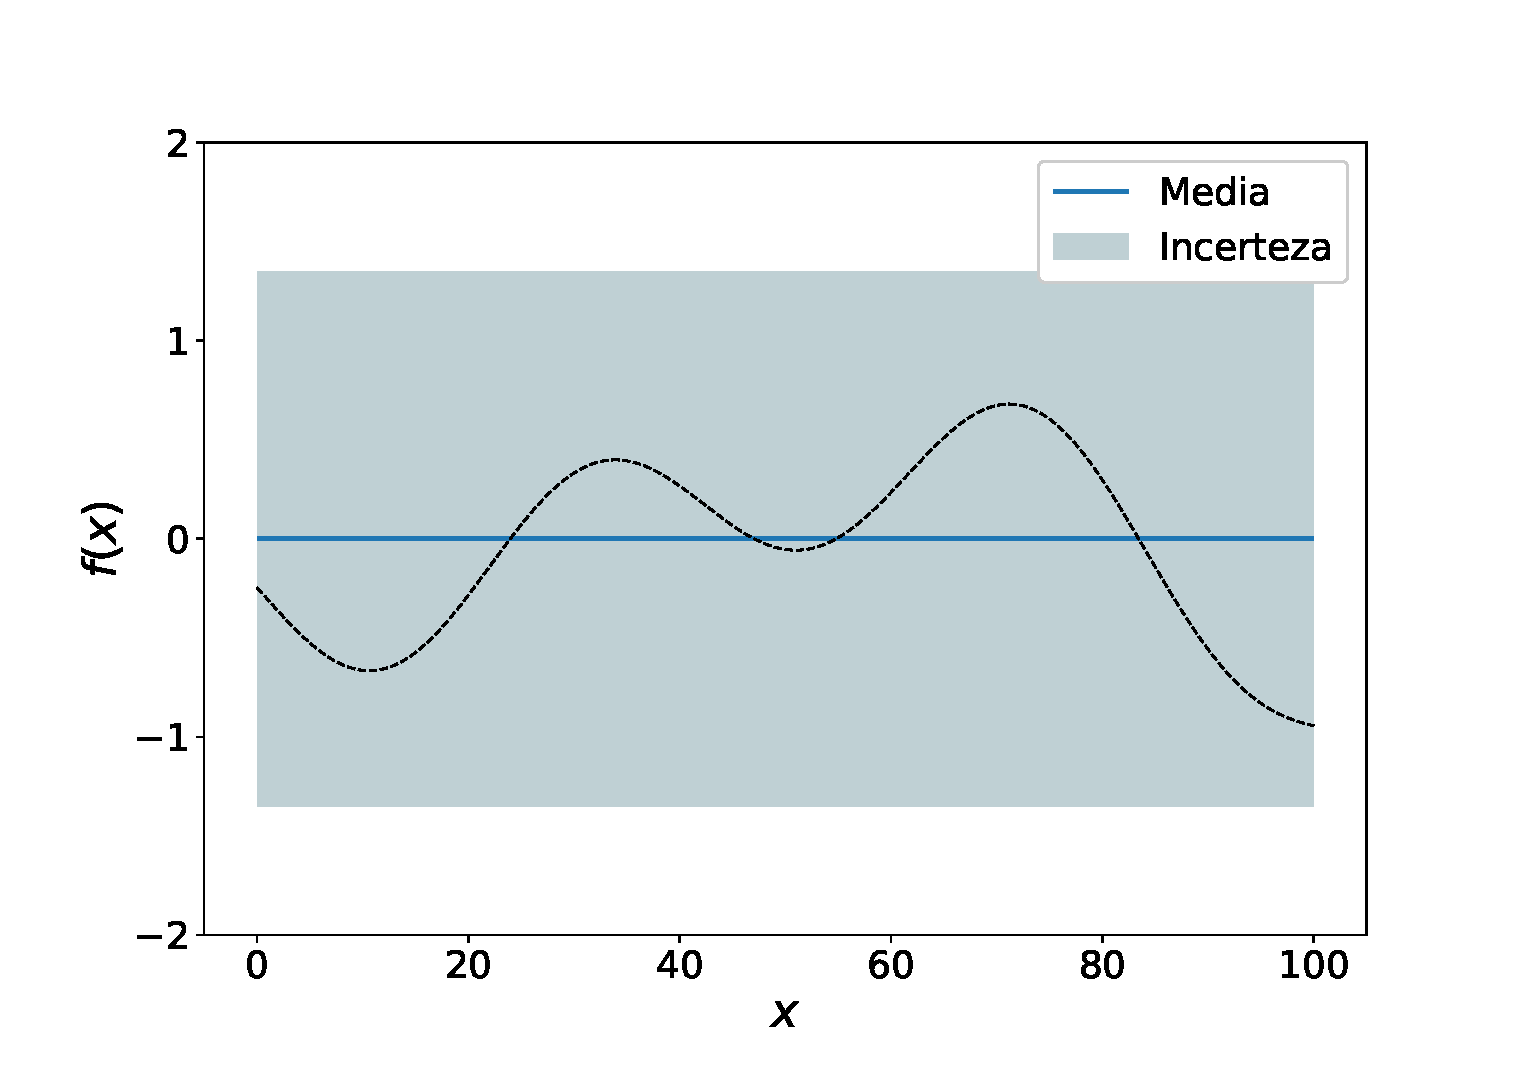
\includegraphics[width=0.31\textwidth]{figures/gp/funcion.eps} 
 \includegraphics[width=0.31\textwidth]{figures/gp/func_acq.eps} 
 \includegraphics[width=0.31\textwidth]{figures/gp/eval1.eps} \\
  \includegraphics[width=0.31\textwidth]{figures/gp/eval2.eps}
  \includegraphics[width=0.31\textwidth]{figures/gp/eval3.eps}
  \includegraphics[width=0.31\textwidth]{figures/gp/eval4.eps} \\
  \includegraphics[width=0.31\textwidth]{figures/gp/eval5.eps}
  \includegraphics[width=0.31\textwidth]{figures/gp/eval6.eps}
  \includegraphics[width=0.31\textwidth]{figures/gp/eval7.eps} 
\end{figure}

\begin{itemize}
\item kernel, 
\item tipo de mapeo, 
\item función de adquisión, 
\item evaluaciones iniciales,
\item costo, 
\item número de evaluaciones.
\end{itemize}

\newpage
%=======================================================================
\section{Resultados}

En esta Sección presentamos los resultados obtenidos de la optimización
del átomo de berilio con estado de carga neutral. Los resultados son 
presentados y analizados en las siguientes subsecciones: energía 
absoluta, energías de excitación, fuerzas de oscilador y secciones 
eficaces de excitación por impacto de electrón. En el ajuste del blanco 
aplicamos el método de optimización bayesiana con procesos gaussianos, 
descrito en la Sección~\ref{sec:gaussianprocess}, mediante la 
implementación del código GPyOpt~\cite{GPyOpt}.

Como hemos establecido en este capítulo, la descripción de los blancos 
atómicos está determinado por tres variables:
\begin{itemize}
\item las configuraciones electrónicas incluidas en el CI,
\item los potenciales modelos definidos en la ecuación radial de 
Schr\"odinger, y
\item los parámetros de escala que definen dichos potenciales.
\end{itemize}
En el presente trabajo, estudiamos la optimización de la estructura 
atómica del Be en el proceso de excitación por impacto de electrón 
considerando solo la última de estas variables. Para ello, definimos a 
priori las configuraciones electrónicas y los modelos potenciales que
modelan dicha estructura. Las configuraciones electrónicas incluidas en
en el modelado de Be a lo largo de esta Sección fueron $2s^2$, $2snl$ 
tal que $n=1$-5 y $l=0$-4, $2p^2$, y $2pnl$ siendo $n=3$-5 y $l=0$-4, 
donde los orbitales $5l$ se han supuesto pseudo-orbitales. Esto resulta 
en un total de 90 términos, donde sólo 19 de ellos son términos 
espectroscópicos. Por otro lado, los potenciales modelos elegidos fueron 
aquellos que mejor describen, sin ningún tipo de ajuste paramétrico, las 
energías y fuerzas de oscilador. Con este criterio, se determinó 
implementar el potencial STO, más un término de intercambio local, y el 
potencial de correlación core-valencia de Norcross.

La optimización de los potenciales y orbitales fue ejecutada en etapas, 
con el fin de comprender en profundidad este proceso. En primera 
instancia, se ajustaron los parámetros que definen el potencial de 
polarización de Norcross. Luego, fijando los parámetros de Norcross 
resultantes, se procedió a ajustar el potencial STO. Para estudiar el 
efecto de la optimización del potencial de Hartree, este procedimiento 
también fue encarado por partes. Cada una de estas partes se corresponde 
a una capa definida por el número cuántico principal $n$. Así, al ajuste 
del potencial STO consistió en optimizar los términos de excitación 
correspondientes a los orbitales $3l$, $4l$ y $5l$, de forma sucesiva y 
manteniendo fijos los parámetros anteriormente optimizados.

Las características del modelo bayesiano fueron consistentes a lo largo 
de todas las optimizaciones de esta Sección; se implementó un mapeo 
inicial tipo latin hypercube, un kernel RBF (square exponential) y una 
función de adquisión de EI. 

%%%%%%%%%%%%%%%%%%%%%%%%%%%%%%%%%%%%%%%%%%%%%%%%%%%%%%%%%%%%%%%%%%%%%%%%%
\subsection{Energía absoluta}
%%%%%%%%%%%%%%%%%%%%%%%%%%%%%%%%%%%%%%%%%%%%%%%%%%%%%%%%%%%%%%%%%%%%%%%%%

La introducción del potencial de polarización de Norcross nos permite
ajustar la energía absoluta del estado fundamental del berilio a su valor 
\textit{experimental}, $E_I=29.336884$ Ry~\cite{NIST}. La ecuación 
(\ref{eq:Norcross-pot}) está compuesta por el conjunto de parámetros 
$\{\alpha_l,\rho_l\}$, donde $l=0,1,2$. Así, se define un espacio 
hiper-paramétrico de seis dimensiones. El parámetro $\alpha$ es la 
polarizabilidad de core. El espacio de búsqueda de esta variable fue 
definido alrededor de su valor experimental \cite{Dalgarno:62,Sitz:71},
%(0.05123~\cite{Dalgarno:62} y 0.05224~\cite{Sitz:71}), 
y dentro de un rango de exploración del 20\%, dado por
\begin{equation}
\boldsymbol\alpha=[0.040-0.060]\,.
\end{equation}
Por otro lado, el parámetro $\rho$ se supone un parámetro de ajuste, por 
lo que nos da más libertad para ajustar la energía de ionización con su 
valor experimental. Así, su rango de exploración fue definido como
\begin{equation}
\boldsymbol\rho=[0.50-1.50]\,.
\end{equation}

La función de costo implementada para ajustar el potencial de 
polarización del core fue definida como
\begin{equation}
J_{\mathrm{pol}} = \sum_{i} \left|\frac{E_{i}-\tilde{E}_{i}
(\boldsymbol{\lambda})}{E_{i}} \right|
\label{eq:Jpol}
\end{equation}
donde $i$ es el índice de los términos incluidos en la optimización, 
$E_{i}$ es la energía absoluta inferida experimentalmente del 
término $i$--ésimo y $\tilde{E}_{i}$ es el valor teórico correspondiente, 
el cual depende de los parámetros $\{\boldsymbol\alpha,\boldsymbol\rho\}$.

El número inicial de evaluaciones fue 6, con un número máximo de 120. Una 
de las grandes dificultades de la minimización u optimización de 
parámetros es la inevitable posibilidad de encontrar un mínimo local. 
Para descartar esta situación, se lanzaron 100 optimizaciones con 
semillas diferentes. Estos cálculos fueron reveladores, ya nos 
permitieron encontrar relaciones subyacentes entre los parámetros y la
naturaleza no-convexa de la superficie hiperdimensional definido por $J$.

% OptI: pol_optI/kernel_test/testE4/
En la primera optimización (Opt. I), consideramos únicamente la energía
absoluta del estado fundamental $2s^2\,^1S$. El 100\% de los cálculos con
semillas aleatorias encontraron un error relativo porcentual menor o 
igual a 0.002\%; mientras que la optimización de 30 semillas conducieron 
a un costo menor o igual a $1\times 10^{-4}$. La tabla~\ref{tab:optpol} 
muestra los mejores resultados hallados. Por otro lado, la distribución 
de los parámetros correspondiente a los mínimos hallados muestran una 
fuerte correlación positiva ($r=0.999$) entre $\alpha $ y $\rho$ para 
$l=0$, mientras que los parámetros para $l=1$ y $l=2$ no muestran 
correlación alguna. Este fenómeno se puede entender teniendo en cuenta 
que sólo el término $2s^2\,^1S$ es incluido en la optimización. A pesar 
de esto, el error relativo de las energías de excitación (respecto al 
estado fundamental) de los 10 términos espectroscópicos restantes fue 
menor al 5\%, con excepción de los términos $2s2p\,^1P$, $2p^2\,^1D$ y 
$2s3d\,^1D$.

\begin{table}
\centering
\begin{tabular}{|*{7}{c|}}
\hline 
$i$ & Término   & NIST & Sin opt.   & Opt. I       & Opt. II      & Opt. III \\
\hline 
\hline 
\rowcolor{mygray} 1 &$2s^2\,^1S$  & $-29.3369$ & $-29.2342$ & $-29.3369$ & $-29.3369$ & $-29.3433$ \\
 & & & $3.5[-1]^\dagger$ & $1.0[-5]$  & $1.0[-4]$  & $2.2[-2]$  \\
\rowcolor{mygray} 2 &$2s2p\,^3P^*$& $-29.1366$ & $-29.0302$ & $-29.1310$ & $-29.1368$ & $-29.1464$ \\
  &       & & $3.7[-1]$  & $1.9[-2]$  & $7.1[-4]$  & $3.4[-2]$  \\
\rowcolor{mygray} 3 &$2s2p\,^1P^*$& $-28.9490$ & $-28.8117$ & $-28.9112$ & $-28.9150$ & $-28.9229$ \\
  &       & & $4.7[-1]$  & $1.3[-1]$  & $1.2[-1]$  & $9.0[-2]$  \\
\rowcolor{mygray} 4 &$2s3s\,^3S$  & $-28.8623$ & $-28.7610$ & $-28.8610$ & $-28.8599$ & $-28.8649$ \\
  &       & & $3.5[-1]$  & $4.3[-3]$  & $8.2[-3]$  & $9.1[-3]$  \\
\rowcolor{mygray} 5 &$2s3s\,^1S$  & $-28.8386$ & $-28.7326$ & $-28.8327$ & $-28.8319$ & $-28.8371$ \\
  &       & & $3.7[-1]$  & $2.0[-2]$  & $2.3[-2]$  & $5.5[-3]$  \\
\rowcolor{mygray} 6 &$2p^2\,^1D$  & $-28.8185$ & $-28.5744$ & $-28.6737$ & $-28.8058$ & $-28.8148$ \\
  &       & & $8.5[-1]$  & $5.0[-1]$  & $4.4[-2]$  & $1.3[-2]$  \\
\hline\multicolumn{3}{c}{$\dagger\,a[b]$ denota $a\times 10^b$} \\
\end{tabular}
\caption[Energías absolutas de Be.]
{Energías absolutas en Rydbergs de los primeros 6 términos espectroscópicos 
de Be (filas superiores) y sus errores relativos porcentuales respecto a 
los valores de NIST (filas inferiores).}
\label{tab:optpol}
\end{table}

% OptI: pol_optII/testE4/
En la segunda optimización (Opt. II) incluimos los términos $2s2p\,^3P^*$ 
y $2s2p\,^1P^*$ en la función de costo dada por la ecuación~(\ref{eq:Jpol}) 
para subsanar la falta de correlación en los parámetros con momento 
angular $l=1$ del potencial de Norcross. Nuevamente, realizamos cálculos 
independientes con 100 semillas diferentes. Los mínimos hallados por cada 
uno de estos cálculos tuvieron una dispersión menor al 0.01\%. El mejor 
resultado hallado se muestra en la tabla~\ref{tab:optpol}. Los errores 
relativos de las energías de excitación de los 10 términos 
espectroscópicos fueron menores al 3\% y en promedio del 1\%, con 
excepción del término $2p^2\,^1P$. Además de la fuerte correlación entre 
$\alpha_0$ y $\rho_0$, la inclusión de los términos correspondientes a la 
configuración $2s2p$ introdujo en la función de costo una fuerte 
correlación entre $\alpha_1$ y $\rho_1$.

Por último (Opt. III), incluimos los términos $2s3s\,^3S$, $2s3s\,^1S$, y 
$2p^2\,^1D$ en la función de costo. El mínimo de la función de costo 
encontrado por cada uno de los 100 cálculos realizados se muestran en la 
figura~\ref{fig:OptIII-100min-Jpol}, mientras que la distribución de los 
parámetros correspondientes a estos mínimos se presentan en la 
figura~\ref{fig:OptIII-100min-params}. Los mínimos hallados tuvieron una 
dispersión menor al 0.01\% alrededor del promedio $\bar{J}=0.17$. El 
mejor resultado de nuestros cálculos se muestra en la 
tabla~\ref{tab:optpol}. Los errores relativos de las energías de 
excitación de los 10 términos espectroscópicos en esta optimización 
fueron menores al 2\% y en promedio del 1\%, nuevamente, a excepción del 
término $2p^2\,^1P$. 

La mejor optimización bayesiana con procesos gaussianos de los parámetros 
$\alpha_l$ y $\rho_l$ se muestra en la figura~\ref{fig:OptIII-Jpol}. Por 
otro lado, la exploración del hiperespacio de parámetros correspondiente
a esta optimización se presenta en la figura~\ref{fig:OptIII-params}. 

%%%% Resultados de 100 optimizaciones 
\begin{figure}[t]
\centering
\includegraphics[width=0.8\textwidth]{figures/rmatrix/OptIII_Jpol.pdf}
\caption[Mínimos de la función de costo según semillas aleatorias.]
{Valores mínimos encontrados para la función de costo~(\ref{eq:Jpol}) 
según 100 cálculos independientes con semillas aleatorias (izquierda) y
su distribución en frecuencia (derecha).}
\label{fig:OptIII-100min-Jpol}
\end{figure}
\begin{figure}[H]
\centering
%\includegraphics[width=0.8\textwidth]{figures/rmatrix/OptIII_params.pdf}
\includegraphics[width=0.8\textwidth]{figures/rmatrix/OptIII_histparams.pdf}
\caption[Distribución de parámetros según semillas aleatorias.]
{Distribución de los parámetros $\alpha_l$ y $\rho_l$ ($l=0,1,2$) 
correspondientes a los valores mínimos que se muestran en la 
figura~(\ref{fig:OptIII-100min-Jpol}).}
\label{fig:OptIII-100min-params}
\end{figure}

%%%% Resultados de la mejor optimización
\begin{figure}[H]
\centering
\includegraphics[width=0.8\textwidth]{figures/rmatrix/OptIII_Jpol_globmin.pdf}
\caption[Minimización de la función de costo.]
{Optimización bayesiana de la función de costo dada por la 
ecuación~(\ref{eq:Jpol}).}
\label{fig:OptIII-Jpol}
\end{figure}
\begin{figure}[H]
\centering
\includegraphics[width=0.8\textwidth]{figures/rmatrix/OptIII_params_globmin.pdf}
\caption[Exploración del espacio de parámetros.]
{Exploración del espacio de parámetros correspondiente a la minimización
dada en la figura~(\ref{fig:OptIII-Jpol}).}
\label{fig:OptIII-params}
\end{figure}

%%%%%%%%%%%%%%%%%%%%%%%%%%%%%%%%%%%%%%%%%%%%%%%%%%%%%%%%%%%%%%%%%%%%%%%%%
\subsection{Energías de excitación}
%%%%%%%%%%%%%%%%%%%%%%%%%%%%%%%%%%%%%%%%%%%%%%%%%%%%%%%%%%%%%%%%%%%%%%%%%

En esta sección estudiamos la optimización de las energías de excitación 
respecto al estado fundamental. En esta etapa de la optimización se 
ajustan los parámetros $\lambda_{nl}$ que definen al potencial modelo STO, 
manteniendo constante los parámetros del potencial de Norcross hallados
en Opt. III. 

La optimización del potencial STO también se realizo por etapas. En 
primer lugar (Opt. $3l$), se consideraron los orbitales $1s$, $2s$, $2p$, 
$3s$, $3p$, $3d$. En segunda instancia (Opt. $4l$), se ajustaron 
adicionalmente los parámetros de escala correspondientes a los orbitales 
$4s$, $4p$, $4d$ y $4f$. Finalmente (Opt. $\bar{5l}$), manteniendo 
constante los $\lambda_{nl}$ encontrados, se ajustaron los parámetros que 
definen los pseudo-orbitales $5s$, $5p$, $5d$, $5f$ y $5g$. Los 
resultados de estas tres optimizaciones se presentan en la 
tabla~\ref{tab:exener}. En todos los casos, la función de costo considera
las energías absolutas de los primeros 11 términos espectroscópicos. 
La energía absoluta del estado fundamental halladas en las optimizaciones 
$3l$, $4l$ y $\bar{5l}$ fueron -29,335167 Ry, -29,33772 Ry, -29,337362 Ry, 
respectivamente, lo que representa una error relativo del 
$6\times 10^{-3}\%$, $4\times 10^{-3}\%$ y $2\times 10^{-3}\%$ respecto
al valor conocido. Una mejor visualización de los resultados de la 
tabla~\ref{tab:exener} se presentan en la figura~\ref{fig:exener}, donde 
se dan los errores relativos de las energías de excitación de los 10 
términos espectroscópicos considerados según las optimizaciones realizadas.
Los valores de las energías de excitación respecto al estado fundamental
son mejorados sistematicamente con las optimizaciones, reduciendo hasta
un orden de magnitud los errores relativos promedios. Los términos más
afectados por la optimización fueron $2s2p\,^1P^*$, $2p^2\,^1D$ y 
$2s3d\,^1D$, que tenian una desviación del 9\%, 27\% y 9\%, respectivamente.
Las optimizaciones $4l$ y $\bar{5l}$ redujeron estos valores hasta menos 
del 2\%, con un promedio del $0.6\%$. 

\begin{table}
\centering
\begin{tabular}{|*{7}{c|}}
\hline 
$i$ & Término    & NIST      & Sin opt.  & Opt. $3l$  & Opt. $4l$  & BO $\bar{5l}$ \\
\hline 
\hline 
1 & $2s^2\,^1S$   & $0.0000$   & $0.0000$   & $0.0000$   & $0.0000$   & $0.0000$ \\
2 & $2s2p\,^3P^*$ & $0.2003$   & $0.2040$   & $0.1987$   & $0.1998$   & $0.1976$ \\
3 & $2s2p\,^1P^*$ & $0.3879$   & $0.4225$   & $0.4185$   & $0.3952$   & $0.3947$ \\
4 & $2s3s\,^3S$   & $0.4746$   & $0.4732$   & $0.4729$   & $0.4714$   & $0.4724$ \\
5 & $2s3s\,^1S$   & $0.4983$   & $0.5016$   & $0.4972$   & $0.4991$   & $0.4985$ \\
6 & $2p^2\,^1D$   & $0.5184$   & $0.6598$   & $0.5296$   & $0.5181$   & $0.5161$ \\
7 & $2s3p\,^3P^*$ & $0.5368$   & $0.5376$   & $0.5345$   & $0.5368$   & $0.5369$ \\
8 & $2p^2\,^3P$   & $0.5440$   & $0.5595$   & $0.5476$   & $0.5537$   & $0.5503$ \\
9 & $2s3p\,^1P^*$ & $0.5485$   & $0.5574$   & $0.5546$   & $0.5493$   & $0.5501$ \\
10 & $2s3d\,^3D$  & $0.5655$   & $0.5665$   & $0.5642$   & $0.5639$   & $0.5647$ \\
11 & $2s3d\,^1D$  & $0.5871$   & $0.5322$   & $0.5924$   & $0.5877$   & $0.5873$ \\
\hline
\end{tabular}
\caption[Energías de excitación de Be.]
{Energía de excitación en Rydbergs de los primeros 11 términos 
espectroscópicos de Be relativos al estado fundamental $2s^2\,^1S$.}
\label{tab:exener}
\end{table}

\begin{figure}[H]
\centering
\includegraphics[width=0.9\textwidth]{figures/rmatrix/erp_ei.pdf} 
\caption[Error relativo de 10 términos espectroscópicos de Be.]
{Error relativo de los primeros 10 términos espectroscópicos respecto 
a valores de NIST.}
\label{fig:exener}
\end{figure}

%%%%%%%%%%%%%%%%%%%%%%%%%%%%%%%%%%%%%%%%%%%%%%%%%%%%%%%%%%%%%%%%%%%%%%%%%
\subsection{Fuerzas de oscilador de asborción}

\begin{table}
\begin{adjustwidth}{-.6in}{-.6in}  
\centering
\begin{tabular}{|*{9}{c|}} 
\hline 
No & Transición                & Ballance   & Chen       & MCHF       & Sin opt.   & BO $3l$    & BO $4l$  & BO $5l$ \\
\hline
\hline
1  & $2s2  \,^1S - 2s2p \,^1P$ & $1.37$     & $1.38$     & $1.38    $ & $1.32    $ & $1.31    $ & $1.40    $ & $1.38$ \\
2  & $2s2  \,^1S - 2s3p \,^1P$ & $1.12[-2]$ & $9.01[-3]$ & $8.99[-3]$ & $5.70[-2]$ & $5.84[-2]$ & $1.71[-2]$ & $1.55[-2]$ \\
3  & $2s2p \,^3P - 2s3s \,^3S$ & $7.56[-2]$ & $8.23[-2]$ & $8.41[-2]$ & $8.57[-2]$ & $8.22[-2]$ & $8.49[-2]$ & $8.21[-2]$ \\
4  & $2s2p \,^3P - 2s3d \,^3D$ & $2.99[-1]$ & $2.95[-1]$ & $3.00[-1]$ & $2.96[-1]$ & $2.67[-1]$ & $3.08[-1]$ & $2.96[-1]$ \\
5  & $2s2p \,^1P - 2s3s \,^1S$ & $1.20[-1]$ & $1.18[-1]$ & $1.15[-1]$ & $1.62[-1]$ & $1.59[-1]$ & $1.23[-1]$ & $1.29[-1]$ \\
6  & $2s2p \,^1P - 2s3d \,^1D$ & $3.86[-1]$ & $4.10[-1]$ & $3.96[-1]$ & $8.18[-2]$ & $2.20[-1]$ & $3.83[-1]$ & $3.74[-1]$ \\
7  & $2s3s \,^3S - 2s3p \,^3P$ & $1.02$     & $1.13    $ & $1.14    $ & $1.15    $ & $1.10$     & $1.13    $ & $1.12$ \\
8  & $2s3s \,^1S - 2s3p \,^1P$ & $9.08[-1]$ & $9.58[-1]$ & $9.47[-1]$ & $9.02[-1]$ & $8.99[-1]$ & $9.80[-1]$ & $9.87[-1]$ \\
9  & $2s3p \,^3P - 2s3d \,^3D$ & $4.83[-1]$ & $5.01[-1]$ & $5.14[-1]$ & $4.92[-1]$ & $5.08[-1]$ & $4.91[-1]$ & $5.18[-1]$ \\
10 & $2s3p \,^1P - 2s3d \,^1D$ & $6.91[-1]$ & $6.87[-1]$ & $6.81[-1]$ & $9.26[-2]$ & $7.74[-1]$ & $7.70[-1]$ & $7.99[-1]$ \\
\hline
\end{tabular}
\caption{Fuerza de oscilador de absorción de transiciones dipolares de Be.}
\label{tab:fabs}
\end{adjustwidth}
\end{table}

\begin{figure}[H]
\centering
%\includegraphics[width=0.9\textwidth]{figures/rmatrix/erp_fabs.pdf} 
\includegraphics[width=0.9\textwidth]{figures/rmatrix/fabs.pdf} 
\caption{Fuerzas de oscilador dipolares de absorción de Be.}
\label{fig:fabs}
\end{figure}

%%%%%%%%%%%%%%%%%%%%%%%%%%%%%%%%%%%%%%%%%%%%%%%%%%%%%%%%%%%%%%%%%%%%%%%%%
\subsection{Excitación por impacto de electrón}

Los resultados obtenidos del cálculo de las secciones eficaces de 
excitación por impacto de electrón en Be se muestran en las 
figuras~\ref{fig:crossBe-partI} y \ref{fig:crossBe-partII}. Las figuras 
muestran las secciones eficaces obtenidas cuando se consideran las 
estructuras atómicas de Be sin optimizar y las optimizadas con procesos
gaussianos (Opt. $3l$, $4l$ y $\hbar{5l}$). 

\begin{figure}[H]
\centering
\includegraphics[width=0.9\textwidth]{figures/rmatrix/GP_RMPS_x6.eps} 
\caption[Secciones eficaces de excitación de Be (Parte I).]
{(Parte I) Secciones eficaces de excitación por impacto de electrón en Be. 
Curvas: Dipti \textit{et al.}~\cite{Dipti:19} (discontinua), RMPS sin 
ajuste (punteada); cálculos con optimización bayesiana: 
$3l$ (raya-punto), 
$4l$ (raya-punto-punto), y
$5l$ (continua). 
Símbolos: cálculos CCC de \cite{Fursa:97}.}
\label{fig:crossBe-partI}
\end{figure}


\begin{figure}[H]
\centering
\includegraphics[width=0.9\textwidth]{figures/rmatrix/GP_RMPS_x4.eps} 
\caption[Secciones eficaces de excitación de Be (Parte II).]
{(Parte II) Secciones eficaces de excitación por impacto de electrón en Be.
Curvas: ídem figura~\ref{fig:crossBe-partI}.}
\label{fig:crossBe-partII}
\end{figure}

\newpage
%=======================================================================
\section{Conclusiones}

\chapter{Conclusiones}
\label{chap:conclusiones}

En este trabajo de investigación se exploró la optimización de sistemas 
multielectrónicos para el cálculo de colisionales inelásticas. Según 
el proceso colisional y la naturaleza del blanco a examinar, se 
implementaron cuatro metodologías diferentes:
\begin{itemize}
\item 
La estructura electrónica de átomos y moléculas se estudió mediante el 
método de inversión depurada (DIM). Esta novedosa aproximación permitió 
obtener potenciales efectivos que describen exitosamente la estructura 
de diversos blancos. Los potenciales DIM se utilizaron, en conjunción 
con dos teorías perturbativas (FBA y CDW), para calcular la ionización 
debido al impacto de proyectiles (fotones y protones). En términos 
generales, el DIM resultó una técnica eficaz para calcular correctamente 
los procesos inelásticos analizados.

\item
Además, se examinó la ionización debido al impacto de iones desnudos en 
blancos moleculares complejos compuestos por H, C, N y O. Para esto, se 
introdujo un modelo estequiométrico simple (SSM), que permite descibir 
una molécula como una combinación lineal de los átomos que la componen. 
A pesar de la simplicidad de este modelo, se demostró que esta 
aproximación es robusta y confiable para predecir a primer orden las 
secciones eficaces de ionización para decenas de sistemas colisionales, 
incluyendo las nucleobases del ADN y ARN. A partir de los cálculos 
realizados, se encontró una ley de escala independiente que permite 
aproximar este proceso para, en principio, cualquier sistemas 
molécula-proyectil.

\item
En el caso de los atómos pesados, se vió la importancia de elegir el 
método apropiado para describir los efectos relativistas. Implementando 
el método de potencial paramétrico de Klapisch y optimizando las 
configuraciones electrónicas elegidas para representar los blancos, se 
obtuvieron estructuras atómicas precisas de lantánidos y metales de 
transición pesados. Se mostró la necesidad de cálculos relativistas
apropiados para predicciones correctamente la fuerza de frenado debido a 
protones en diversos blancos.

\item
En la última parte de este trabajo, se examinó la excitación por impacto 
de electrones de átomos neutros mediante el método de $R$-matrix. 
En este caso, el esquema de optimización de la estructura atómica 
depende del ajuste manual de los parámetros del problema. 
La complejidad del cálculo se resolvió empleando la optimización 
Bayesiana mediante procesos Gaussianos, que permitió ajustar de forma 
automática la estructura del blanco. Esta implementación mostró 
ser un éxito tanto para reproducir la estructura del blanco (energías 
de excitación, totales y oscillator strengths) como las secciones 
eficaces de excitación, con un costo computacional relativamente bajo.
\end{itemize}
%
Las metodologías empleadas en esta Tesis permitieron calcular de forma 
precisa la estructura electrónica de una amplia variedad de sistemas 
atómicos y moleculares. Estos blancos se examinaron en procesos 
inelásticos descriptos mediante métodos teóricos con diferentes órdenes 
de aproximación --desde aproximaciones perturbativas de primer orden 
hasta métodos completamente cuánticos. Del trabajo presentado se 
concluye que sólo mediante la correcta optimización de los blancos se 
puede calcular de forma precisa, en el rango de validez definido, los 
procesos inelásticos a los que estos son sometidos.



\chapter*{Publicaciones asociadas}
\label{chap:publicaciones}

\begin{enumerate}

\item
A.M.P. Mendez, D.M. Mitnik, J.E. Miraglia,
\textit{Depurated Inversion Method for Orbital-Specific Exchange Potentials},
Int. J. Quantum. Chem. \textbf{116}, 1882 (2016). \\
DOI:~\href{http://www.doi.org/10.1002/qua.25295}{10.1002/qua.25295}

\item
A.M.P. Mendez, D.M. Mitnik, J.E. Miraglia, 
\textit{Local Effective Hartree-Fock Potentials Obtained by the Depurated Inversion Method},
Adv. Quant. Chem. \textbf{76}, 117--132 (2018). \\
DOI:~\href{http://www.doi.org/10.1016/bs.aiq.2017.07.004}{10.1016/bs.aiq.2017.07.004}

\item
A.M.P. Mendez, D.M. Mitnik, J.E. Miraglia, 
\textit{Collision processes using effective potentials},
Adv. Quant. Chem. \textbf{79}, 179--200 (2019). \\
DOI:~\href{http://www.doi.org/10.1016/bs.aiq.2019.05.003}{10.1016/bs.aiq.2019.05.003}

\item
D.M. Mitnik, A.M.P. Mendez, J.E. Miraglia, 
\textit{Reply to ``Comment on `Depurated Inversion Method for Orbital-Specific
Exchange Potentials' ''}, 
Int. J. Quantum Chem. \textbf{120}, e26102 (2019). \\
DOI:~\href{http://www.doi.org/10.1002/qua.26102}{10.1002/qua.26102}

\item
A.M.P. Mendez, C.C. Montanari, D.M. Mitnik, 
\textit{Relativistic atomic structure calculations of heavy targets for inelastic collisions},
Nucl. Instrum. Methods Phys. Res. B, \textbf{460}, 114-118 (2019). \\
DOI:~\href{http://www.doi.org/10.1016/j.nimb.2019.02.002}{10.1016/j.nimb.2019.02.002}

\item
C.C. Montanari, P. A. Miranda, E. Alves, A. M. P. Mendez \textit{et al.},
\textit{Stopping power of hydrogen in hafnium and the importance of relativistic 4f electrons},
Phys. Rev. A \textbf{101}, 062701 (2020). \\
DOI:~\href{http://www.doi.org/10.1103/PhysRevA.101.062701}{10.1103/PhysRevA.101.062701} \\ \\

\item
M. Oswald, S. Kumar, U. Singh, G. Singh, K.P.Singh, D. Mehta, A. Mendez 
\textit{et al.}, 
\textit{Experimental and theoretical L-shell ionization cross sections of heavy atoms by impact of Si ions},
Radiat. Phys. Chem.  \textbf{176}, 108809 (2020). \\
DOI:~\href{http://www.doi.org/10.1016/j.radphyschem.2020.108809}{10.1016/j.radphyschem.2020.108809}

\item
A.M.P. Mendez, C.C. Montanari, J.E. Miraglia,
\textit{Ionization of biological molecules by multicharged ions using the stoichiometric model},
J. Phys. B, \textbf{53}, 055201 (2020). \\
DOI:~\href{http://www.doi.org/10.1088/1361-6455/ab6052}{10.1088/1361-6455/ab6052}

\item
A.M.P. Mendez, C.C. Montanari, J.E. Miraglia,
\textit{Scaling rules for the ionization of biological molecules by highly charged ions},
J. Phys. B, \textbf{53}, 175202 (2020). \\
DOI:~\href{http://www.doi.org/10.1088/1361-6455/ab9c36}{10.1088/1361-6455/ab9c36}

\item
A.M.P. Mendez, J.I. Di Filippo, S.D. López, D.M. Mitnik,
\textit{Bayesian atomic structure calculations for collisional problems},
J. Phys.: Conf. Ser. \textbf{1412}, 132027 (2020). \\
DOI:~\href{http://www.doi.org/10.1088/1742-6596/1412/13/132027}{10.1088/1742-6596/1412/13/132027}

\end{enumerate}


\appendix

%%%%%%%%%%%%%%%%%%%%%%%%%%%%%%%%%%%%%%%%%%%%%%%%%%%%%%%%%%%%%%%%%%%%%%%
\chapter{Primera aproximación de Born}
\label{app:born}

%%%%%%%%%%%%%%%%%%%%%%%%%%%%%%%%%%%%%%%%%%%%%%%%%%%%%%%%%%%%%%%%%%%%%%%
\chapter{Ecuación normal}
\label{app:ecnormal}

Las semillas iniciales dadas por la ecuación normal se obtienen al 
minimizar la función
\begin{equation}
 \beta(x_i) = y(x_i) - f(x_i,\lambda_1,\lambda_2,\cdots,\lambda_m)\,,
\end{equation}
que es la diferencia entre la curva a ser ajustada, $y(r)$, y la función
analítica implementada para tal fin, $f(r)$. En el esquema de la inversión
depurada, $y(r) = Z_{nl}^{\mathrm{HF}}(r)$ corresponde a la carga invertida,
y $f(r) = Z_{nl}^{\mathrm{DIM}}(r)$ corresponde a la forma analítica que 
se ha fijado para la carga (la ecuación \ref{eq:atomzDIM} para átomos y 
la ecuación \ref{eq:molzDIM} para moléculas). Con el fin de minimizar
$\beta(x_i)$ respecto a los $m$ parámetros $\lambda_j$ que determinan 
$f$, definimos los elementos de matriz $A_{ij}$,
\begin{equation}
  A_{ij} \equiv \frac{d\beta(x_i)}{d\lambda_j} =
 \frac{df(x_i,\lambda_1,\lambda_2,\cdots, \lambda_m)}{d\lambda_j}
\end{equation}
Así, obtenemos el sistema de ecuaciones
\begin{equation}
 \left[
 \begin{array}{c}
  d\beta(x_1) \\
  d\beta(x_2) \\
  \vdots \\
  d\beta(x_n) \\
 \end{array}
 \right] =
 \left[
 \begin{array}{cccc}
  A_{11} & A_{12} & \cdots & A_{1m} \\
  A_{21} & A_{22} & \cdots & A_{2m} \\
  \vdots & \vdots & \ddots & \vdots \\
  A_{n1} & A_{n2} & \cdots & A_{nm} \\
 \end{array}
 \right]
 \left[
 \begin{array}{c}
 d\lambda_1 \\
 d\lambda_2 \\
 \vdots \\
 d\lambda_m \\
 \end{array}
 \right] \,.
\end{equation}
Multiplicando ambos lados de la ecuación por la matrix traspuesta $[A]^{T}$,
\begin{equation}
  \left[ A \right]^T \left[ A \right]\left[ d\lambda \right] =
  \left[ A \right]^T \left[ d\beta \right]\,,
\end{equation}
se obtiene un sistema de ecuaciones que se resuelve con rutinas numéricas 
estándar. Así, la solución $[d\lambda]$ permite obtener los parámetros 
iniciales que minimizan $[\beta]$.

%%%%%%%%%%%%%%%%%%%%%%%%%%%%%%%%%%%%%%%%%%%%%%%%%%%%%%%%%%%%%%%%%%%%%%%
\chapter{Método de onda continua distorsionada (CDW)}
\label{app:CDW}

%%%%%%%%%%%%%%%%%%%%%%%%%%%%%%%%%%%%%%%%%%%%%%%%%%%%%%%%%%%%%%%%%%%%%%%
\chapter{Modelo de potencial apantallado con condición de cúspide}
\label{app:SPCC}

%%%%%%%%%%%%%%%%%%%%%%%%%%%%%%%%%%%%%%%%%%%%%%%%%%%%%%%%%%%%%%%%%%%%%%%
\chapter{Formalismo dieléctrico de Mermin--Lindhard}
\label{app:ML}

%%%%%%%%%%%%%%%%%%%%%%%%%%%%%%%%%%%%%%%%%%%%%%%%%%%%%%%%%%%%%%%%%%%%%%%
\chapter{Aproximación de plasma local por capa}
\label{app:SLPA}

%%%%%%%%%%%%%%%%%%%%%%%%%%%%%%%%%%%%%%%%%%%%%%%%%%%%%%%%%%%%%%%%%%%%%%%
\chapter{Método de R-Matrix}
\label{app:rmatrix}

\section{R--Matrix con pseudo--estados}
\label{app:RMPS}

El método de R--Matrix con pseudo--estados (\acs{rmps}) ...


 

\begin{thebibliography}{9}

%%%%%%%%%%%%%%%%%%%%%%%%%%%%%%%%%%%%%%%%%%%%%%%%%%%%%%%%%%%%%%%%%%%%%%%%
% CAPITULO 2
%%%%%%%%%%%%%%%%%%%%%%%%%%%%%%%%%%%%%%%%%%%%%%%%%%%%%%%%%%%%%%%%%%%%%%%%

% Introducción

\bibitem{HohenberKohn:64}
P. Hohenberg, W. Kohn, 
Phys. Rev. 1964, 136, B864

\bibitem{KohnSham:65}
W. Kohn, L. J. Sham, 
Phys. Rev. 1965, 140, A1133

\bibitem{Becke:14} 
A. D. Becke,
J. Chem. Phys. 2014, 140, 18A301.

\bibitem{Bartlett:10} 
R. J. Bartlett, 
Mol. Phys. 2010, 108, 3299-3311.

\bibitem{Verma:12} 
P. Verma, R. J. Bartlett,
J. Chem. Phys. 2012, 137, 134102.

\bibitem{Slater:51}
J. C. Slater, 
Phys. Rev. 1981, 81, 385.

\bibitem{Sharp:53} 
R. T. Sharp, G. K. Horton,
Phys. Rev. 1953, 90, 317.

\bibitem{Talman:76} 
J. D. Talman, W. F. Shadwick, 
Phys. Rev. A 1976, 14, 36-40.

\bibitem{Talman:89} 
J. D. Talman, 
Comput. Phys. Commun. 1989, 54, 85-94.

\bibitem{Krieger:92}
J. B. Krieger, Y. Li, G. J. Iafrate, 
Phys. Rev. A 1992, 45, 101-126.

\bibitem{Gorling:92}
A. G\"orling,
Phys. Rev. A 1992, 46, 3753-3757.

\bibitem{Yang:02}
W. Yang, Q. Wu,
Phys. Rev. Lett. 2002, 89, 143002.

\bibitem{Staroverov:06}
V. N. Staroverov, G. E. Scuseria and E. R. Davidson,
J. Chem. Phys. 2006, 124, 11103.

\bibitem{Ryabinkin:13}
I. G. Ryabinkin, A. A. Kananenka, and V. N. Staroverov,
Phys. Rev. Lett. 2013, 111, 013001.

\bibitem{abinit}
{\sc abinit},  
\url{www.abinit.org}

\bibitem{Vanderbilt}
Vanderbilt Ultra--Soft Pseudopotential,  
\url{www.physics.rutgers.edu/~dhv/uspp/}

\bibitem{Gaiduk:13}
A. P. Gaiduk, I. G. Ryabinkin, V. N. Staroverov,
J. Chem. Theory Comput. 2013, 9, 3959.

\bibitem{Wu:03}
Q. Wu, W. Yang,
J. Chem. Phys. 2003, 118, 2498.

\bibitem{Ryabinkin:15}
I. G. Ryabinkin, S. V. Kohut, V. N. Staroverov,
Phys. Rev. Lett. 2015, 115, 083001.

\bibitem{Mura:97} 
M. E. Mura, P. J. Knowles, C. A. Reynolds,
J. Chem. Phys. 1997, 106, 9659.

\bibitem{Umrigar:94} 
C. J. Umrigar, X. Gonze,
Phys. Rev. A 1994, 50, 3827.

\bibitem{Gritsenko:97} 
O. V. Gritsenko, E. J. Baerends, 
Theor. Chem. Acc. 1997, 96, 44.

\bibitem{Filippi:94} 
C. Filippi, C. J. Umrigar, M. Taut, 
J. Chem. Phys. 1994, 100, 1290.

\bibitem{Schipper:97} 
P. R. T. Schipper, O. V. Gritsenko, E. J. Baerends,
Theor. Chem. Acc. 1997, 98, 16.

\bibitem{deSilva:12}
P. de Silva, T. A. Wesolowski,
Phys. Rev. A 2012, 85, 032518.

\bibitem{Kananenka:13} 
A. A. Kananenka, S. V. Kohut, A. P. Gaiduk, and I. G. Ryabinkin, 
J. Chem. Phys. 2013, 139, 074112.

\bibitem{Jacob:11} 
C. R. Jacob,
J. Chem. Phys. 2011, 135, 244102.

\bibitem{Hilton:77} 
P. R. Hilton, S. Nordholm, N. S. Hush, 
J. Chem. Phys. 1997, 67, 5213.

\bibitem{Suzer:77} 
S. S{\"u}zer, P. R. Hilton, N. S. Hush, S. Nordholm,
J. Elect. Spec. Rel. Phen. 1977, 12, 357.

\bibitem{Hilton:79} 
P. R. Hilton, S. Nordholm, N. S. Hush,
Chem. Phys. Lett. 1979, 64, 515.

\bibitem{Hilton:80} 
P. R. Hilton, S. Nordholm, N. S. Hush, 
J. Elect. Spec. Rel. Phen. 1980, 18, 101.

\bibitem{Crljen:87} 
{\v Z}. Crljen, G. Wendin,
Phys. Rev. A 1987, 35, 1571.

\bibitem{Sternheimer:54} 
R. M. Sternheimer, 
Phys. Rev. 1954, 96, 951.

\bibitem{Dalgarno:59} 
A. Dalgarno, D. Parkinson,
Proc. R. Soc. Lond. A 1959, 250, 422.

\bibitem{Mendez:16}
A. M. P. Mendez, D. M. Mitnik, J. E. Miraglia, 
Int. J. Quantum Chem. \textbf{116}, 1882--1890 (2016).

\bibitem{Mendez:18}
Mendez, A. M. P.; Mitnik, D. M.; Miraglia, J. E. 
Local Effective Hartree--Fock Potentials Obtained by the Depurated Inversion Method. 
In {\it Nov. Electron. Struct. Theory Gen. Innov. Strongly Correl. Syst.}; 
Hoggan, P. E., Ed.; 
Advances in Quantum Chemistry;
Academic Press, 2018;
Vol.~76; pp~117--132.

\bibitem{Bates:62}
Bates, D. R.; 
Theoretical Treatment of Collisions between Atomic Systems.
In {\it At. Mol. Process.};
Bates, D. R., Ed;
Pure and Applied Physics;
Elsevier, 1962;
Vol.~13, pp 549--621.

\bibitem{McDowell:61}
McDowell, M. R. C.; Peach, G.
Ionization of Lithium by Fast Protons and Electrons.
{\it Phys. Rev.} {\bf 1961}, 121, 1383--1387.

\bibitem{Pindzola:07}
Pindzola, M. S.; Robicheaux, F.; Loch, S. D.; Berengut,  J. C.; Topcu, T.; Colgan, J.; Foster, M.; Griffin, D. C.; Ballance, C. P.; Schultz, D. R.;
Minami, T.; Badnell, N. R.; Witthoeft, M. C.; Plante, D. R.; Mitnik, D. M.; 
Ludlow, J. A.; Kleiman, U.
%The time-dependent close-coupling method for  atomic and molecular collision processes.
{\it J. Phys. B}, {\bf 2007}, 40, R39-R60.

\bibitem{Burke:11}
Burke, P. G.
{\it R--Matrix Theory of Atomic Collisions.}
Springer--Verlag Berlin Heidelberg, 2011.

\bibitem{Bray:17}
Bray, I; Abdurakhmanov, I. B.; Bailey, J. J.; Bray, A. W.; Fursa, D. V.;
Kadyrov, A. S.; Rawlins, C. M.; Savage, J. S.; Stelbovics, A. T.; Zammit, M. C.
%Convergent close--coupling approach to light and heavy projectile scattering on atomic and molecular hydrogen.
{\it J. Phy. B}, {\bf 2017}, 50, 202001. 

\bibitem{Pindzola:16}
Pindzola, M. S.; Colgan, J.; Robicheaux, F.; Lee, T.-G.; Ciappina, M. F.;
Foster, M.; Ludlow, J. A.; Abdel-Naby, S. A.
Time-Dependent Close--Coupling Calculations for Ion--Impact Ionization of Atoms and Molecules. 
In {\it Advances In Atomic, Molecular, and Optical Physics};
Arimondo, E.; Lin, C. C.; Yelin, S. F., Ed,; 
Academic Press, 2016; Vol. 65,; pp 291--319.

\bibitem{Szabo:96}
Szabo, A.; Ostlund, N. S.
{\it Modern Quantum Chemistry: Introduction to Advanced Electronic 
Structure Theory},
Dover Publications, Inc.: Mineola, New York, 1996.

\bibitem{Helgaker:00}
Helgaker, T.; J{\o}rgensen, P.; Olsen, J.
{\it Molecular Electronic-Structure Theory},
John Wiley {\&} Sons, Ltd: Chichester, UK, 2000.

\bibitem{Schaefer:04}
Schaefer, H. F. III
{\it Quantum Chemistry: The Development of Ab Initio Methods in
Molecular Electronic Structure Theory},
Dover Publications, Inc: Mineola, New York, 2004.


\begin{comment}

% atomos hidrogenicos

\bibitem{Cowan1981} 
R.D. Cowan, {\it The Theory of Atomic Structure and Spectra}, 
University of California Press (1981). 

\bibitem{Brandsen1983} 
B.H. Brandsen and C.J. Joachin, 
{\it Physics of atoms and molecules}, 
Longman Scientific and Technical (1984).

\end{comment}

\bibitem{FroeseFischer:97}
Froese Fischer, C.; Brage, T.; J\"onsson, P.
{\it Computational Atomic Structure: An MCHF Approach},
Institute of Physics Publishing: Bristol, UK, 1997.

\bibitem{Johnson:07}
Johnson, W. R. 
{\it Atomic Structure Theory: Lectures on Atomic Physics},
Springer--Verlag Berlin Heidelberg, 2007.

\bibitem{Albright:93} 
Albright, B.J.; Bartschat, K.; Flicek, P.R.
J. Phys. B 1993, 26, 337.

\bibitem{Bartschat:96} 
Bartschat, K. 
Computational Atomic Physics,
Springer--Verlag, 1996; Chapter II.

\bibitem{BartschatBray:96} 
Bartschat, K.; Bray, I.
J. Phys. B 1996, 29, 271.

% dim en moleculas

\bibitem{Schipper1997}
Schipper, P. R. T.; Gritsenko, O. V.; Baerends, E. J. 
Kohn-Sham potentials corresponding to Slater and Gaussian basis set densities.
{\it Theor. Chem. Accounts: Theory, Comput. Model. (Theoretica Chim. Acta)} {\bf 1997}, 98, 16--24.

\bibitem{Mura1997}
Mura, M. E.; Knowles, P. J.; Reynolds, C. A.
Accurate numerical determination of Kohn--Sham potentials from electronic densities: I. Two--electron systems.
{\it J. Chem. Phys.} {\bf 1997}, 106, 9659--9667.

\bibitem{Jacob2011}
Jacob, C. R. 
Unambiguous optimization of effective potentials in finite basis sets.
{\it J. Chem. Phys.} {\bf 2011}, 135, 244102.

\bibitem{Gaiduk2013}
Gaiduk, A. P.; Ryabinkin, I. G.; Staroverov, V. N.
Removal of Basis--Set Artifacts in Kohn--Sham Potentials Recovered from Electron Densities.
{\it J. Chem. Theory Comput.} {\bf 2013}, 9, 3959--3964.

\bibitem{Schmidt1993}
Schmidt, M. W.; Baldridge, K. K.; Boatz, J. A.; Elbert, S. T.; Gordon, M. S.; Jensen, J. H.; Koseki, S.;
Matsunaga, N.; Nguyen, K. A.; Su, S.; Windus, T. L.; Dupuis, M.; Montgomery, J. A.
General atomic and molecular electronic structure system.
{\it J. Comput. Chem.} {\bf 1993}, 14, 1347--1363.

\bibitem{Gordon2005}
Gordon, M. S.; Schmidt, M. W.
Advances in electronic structure theory: GAMESS a decade later. 
In {\it Theory Appl. Comput. Chem.}; 
Dykstra, C. E.; Frenking, G.; Kim, K. S.; Scuseria, G. E. Eds;
Elsevier: Amsterdam, 2005; pp 1167--1189.

% experimentos fotoionizacion de N y Ne

\bibitem{Henke1993}
Henke, B. L.; Gullikson, E. M.; Davis, J. C. 
X--Ray Interactions: Photoabsorption, Scattering, Transmission, and Reflection at $E$=50--30000 eV, $Z$=1--92.
{\it At. Data Nucl. Data Tables} {\bf 1993}, 54, 181--342.

\bibitem{Samson1990}
Samson, J. A. R.; Angel, G. C.
Single-- and double--photoionization cross sections of atomic nitrogen from threshold to 31 \AA.
{\it Phys. Rev. A} {\bf 1990}, 42, 1307--1312.

\bibitem{Samson2002}
Samson, J. A. R.; Stolte, W. C.
Precision measurements of the total photoionization cross--sections of He, Ne, Ar, Kr, and Xe.
{\it J. Electron Spectros. Relat. Phenomena} {\bf 2002}, 123, 265--276.

\bibitem{Stolte2016}
Stolte, W. C.; Jonauskas, V.; Lindle, D. W.; Sant'Anna, M. M.; Savin, D. W. 
Inner--shell Photoionization studies of neutral atomic nitrogen.
{\it Astrophys. J.} {\bf 2016}, 818, 149.

\bibitem{Ederer1964}
Ederer, D. L. 
Photoionization of the $4d$ electrons in Xenon.
{\it Phys. Rev. Lett.} {\bf 1964}, 13, 760--762.

% experimentos fotoionizacion ch4

\bibitem{Granados2016}
Granados--Castro, C. M.
Application of Generalized Sturmian Basis Functions to Molecular Systems.
Ph.D. Thesis, Universit\'e de Lorraine, Metz, France and 
Universidad Nacional del Sur, Bah\'ia Blanca, Argentina, 2016.

\bibitem{Rothenberg1971}
Rothenberg, S.; Schaefer, H. F.
Methane as a Numerical Experiment for Polarization Basis Function Selection.
{\it J. Chem. Phys.} {\bf 1971}, 54, 2764--2766.

\bibitem{Hariharan1972}
Hariharan, P. C.; Pople, J. A.
The effect of d-functions on molecular orbital energies for hydrocarbons.
{\it Chem. Phys. Lett.} {\bf 1972}, 16, 217--219.

\bibitem{Lukirskii1964}
Lukirskii, A. P.; Brytov, I. A.; Zimkina, T. M.
{\it Optika i spektr.} {\bf 1964}, 17, 234.

\bibitem{Henke1982}
Henke, B. L.; Lee, P.; Tanaka, T. J.; Shimabukuro, R. L.; Fujikawa, B. K.
Low--energy X--ray interaction coefficients: Photoabsorption, scattering, and reflection: $E$=100--2000 eV $Z$=1--94.
{\it At. Data Nucl. Data Tables} {\bf 1982}, 27, 1--144.

\bibitem{Samson1989}
Samson, J. A. R.; Haddad, G. N.; Masuoka, T.; Pareek, P. N.; Kilcoyne, D. A. L.
Ionization yields, total absorption, and dissociative photoionization cross sections of CH$_4$ from 110 to 950 \AA.
{\it J. Chem. Phys.} {\bf 1989}, 90, 6925--6932.

% experimentos ionizacion ch4

\bibitem{Rudd1983}
Rudd, M. E.; DuBois, R. D.; Toburen, L. H.; Ratcliffe, C. A.; Goffe, T. V.
Cross sections for ionization of gases by 5--4000 keV protons and for electron capture by 5--150 keV protons.
{\it Phys. Rev. A} {\bf 1983}, 28, 3244--3257.

\bibitem{Rudd1985}
Rudd, M. E.; Kim, Y. K.; Madison, D. H.; Gallagher, J. W.
Electron production in proton collisions: total cross sections.
{\it Rev. Mod. Phys.} {\bf 1985}, 57, 965--994.

%%%%%%%%%%%%%%%%%%%%%%%%%%%%%%%%%%%%%%%%%%%%%%%%%%%%%%%%%%%%%%%%%%%%%%%%
% IONIZACION DE MOLECULAS: MODELO ESTEQUIOMETRICO
%%%%%%%%%%%%%%%%%%%%%%%%%%%%%%%%%%%%%%%%%%%%%%%%%%%%%%%%%%%%%%%%%%%%%%%%

\bibitem{Mohamad2017}
O. Mohamad, B. J. Sishc, J. Saha, A. Pompos, A. Rahimi, M. D. Story, A. J. Davis, D. N. Kim, 
%Carbon Ion Radiotherapy: A Review of Clinical Experiences and Preclinical Research, with an Emphasis on DNA Damage/Repair. 
Cancers \textbf{9}, 66 (2017).

\bibitem{galassi2000}
M. E. Galasssi, R. D. Rivarola, M. Beuve, G. H. Olivera and P. D. Fainstein, 
Phys. Rev. A \textbf{62}, 022701 (2000).

\bibitem{ludde2016}
H. J. L\"udde, A. Achenbach, T. Kalkbrenner, H.-C. Jankowiak and T. Kirchner,
Eur. Phys. J. D \textbf{70}, 82 (2016).

\bibitem{ludde2018}
H. J. L\"udde, M. Horbatsch and T. Kirchner,
Eur. Phys. J. B \textbf{91}, 99 (2018).

\bibitem{fainstein1988}
Fainstein P.D., Ponce V. H. and Rivarola R. D. 
J. Phys. B: At. Mol. Opt. Phys. \textbf{21} 287 (1988).

\bibitem{miraglia2008} 
J. E. Miraglia and M. S. Gravielle. 
%Ionization of the He, Ne, Ar, Kr, and Xe isoelectronic series by proton impact. 
Phys Rev A \textbf{78}, 052705 (2008)

\bibitem{miraglia2009} 
J. E. Miraglia, 
%Ionization of He, Ne, Ar, Kr, and Xe by proton impact: Single differential distributions. 
Phys. Rev. A \textbf{79}, 022708 (2009).

\bibitem{Denifl2011}
Denifl S., Märk T.D., Scheier P. 
The Role of Secondary Electrons in Radiation Damage. 
In Radiation Damage in Biomolecular Systems. Biological and Medical Physics, Biomedical Engineering. 
Eds: García Gómez-Tejedor G., Fuss M. 
Springer, Dordrecht (2012) 

\bibitem{toburen1975} 
W. E. Wilson and L. H. Toburen. 
%Electron emission from proton --hydrocarbon-molecule collisions at 0.3--2.0 MeV. 
Phys. Rev. A \textbf{11}, 1303 (1975).

\bibitem{toburen1976} 
D. J. Lynch, L. H. Toburen, and W. E. Wilson. 
%Electron emission from methane, ammonia, monomethylamine, and dimethylamine by 0.25 to 2.0 MeV protons. 
J. Chem. Phys. \textbf{64}, 2616 (1976).

\bibitem{gamess}
M. W. Schmidt, K. K. Baldridge, J. A. Boatz, S. T. Elbert, M. S. Gordon, 
J. H. Jensen, S. Koseki, N. Matsunaga, K. A. Nguyen, S. J. Su, T. L. Windus, 
M. Dupuis, J. A. Montgomery 
J. Comput. Chem. \textbf{14}, 1347-1363 (1993).

\bibitem{salvat1995}
Salvat, F., Fern\'andez-Varea, J.M., Williamson, W.
Comput. Phys. Commun. \textbf{90}, 151--168 (1995)

\bibitem{montanari2017} 
C. C. Montanari, J. E. Miraglia,
%Ionization probabilities of Ne, Ar, Kr, and Xe by proton impact for different initial states and impact energies. 
Nucl. Instr. Meth. Phys. Res. B \textbf{407}, 236--243 (2017).

\bibitem{miraglia2019} 
J. E. Miraglia,
%Shell-to-shell ionization cross sections of antiprotons, H$^{+}$, He$^{2+},$ Be$^{4+},$ C$^{6+}$ and 
%O$^{8+}$ on H, C, N, O, P, and S atoms (to be published).

\bibitem{surdutovic2018} 
E. Surdutovich and A. V. Solov'yov, 
%Multiscale approach to the physics of radiation damage with ions. 
arXiv:1312.0897v, (2013)

\bibitem{abril2015} 
P. de Vera, I. Abril, R. Garcia-Molina and A. V. Solov'yov,
%Ionization of biomolecular targets by ion impact: input data for radiobiological applications. 
Journal of Physics: Conference Series \textbf{438}, 012015 (2013).

\bibitem{Rudd1992} 
M. E. Rudd, Y.-K. Kim,, D. H. Madison and T. J. Gay.
%Electron production in proton collisions with atoms and molecules: energy distributions. 
Rev. Mod. Phys. \textbf{64}, 441--490 (1992).

\bibitem{iriki2011}
Y. Iriki, Y. Kikuchi, M. Imai, and A. Itoh
Phys. Rev. A \textbf{84}, 052719 (2011).

\bibitem{rahman2016}
M. A. Rahman and E. Krishnakumar,
Electron ionization of DNA bases,
J. Chem. Phys. \textbf{144}, 161102 (2016).

\bibitem{mozejko2003}
P. Mozejko and L. Sanche, 
%Cross section calculations for electron scattering from DNA and RNA bases.
Radiat Environ. Biophys \textbf{42}, 201 (2003).

\bibitem{tan2018}
H. Q. Tan, Z. Mi, and A. A. Bettiol, 
%Simple and universal model for electron-impact ionization of complex biomolecules, 
Phys. Rev. E \textbf{97}, 032403 (2018)

\bibitem{itoh2013} 
A. Itoh, Y. Iriki, M. Imai, C. Champion, and R. D. Rivarola, 
%Cross sections for ionization of uracil by MeV-energy-proton impact, 
Phys. Rev. A \textbf{88}, 052711 (2013).

\bibitem{agnihotri2012}
A. N. Agnihotri, S. Kasthurirangan, S. Nandi, A.
Kumar, M. E. Galassi, R. D. Rivarola, O. Foj\'{o}n, C. Champion, J. Hanssen,
H. Lekadir, P. F. Weck, and L. C. Tribedi. 
%Ionization of uracil in collisions with highly charged carbon and oxygen ions of energy 100 keV to 78 MeV. 
Phys. Rev. A \textbf{85}, 032711 (2012).

\bibitem{agnihotri2013}
A N Agnihotri, S Kasthurirangan, S Nandi, A Kumar, C Champion,, H Lekadir, 
J Hanssen, P FWeck, M E Galassi, R D Rivarola, O Fojon and L C Tribedi, 
%Absolute total ionization cross sections of uracil (C$_4$H$_4$N$_2$O$_2$) in collisions with MeV energy highly charged carbon, oxygen and fluorine ions
J. Phys. B \textbf{46}, 185201 (2013).

\bibitem{champion2012} 
C Champion, M E Galassi, O Foj\'{o}n, H Lekadir, J Hanssen, R D Rivarola,
P F Weck, A N Agnihotri, S Nandi, and L C Tribedi. 
%Ionization of RNA-uracil by highly charged carbon ions.
J. Phys.: Conf. Ser. \textbf{373}, 012004 (2012).

\bibitem{wolff2014}
W. Wolff, H. Luna, L. Sigaud, A. C. Tavares, and E. C. Montenegro
%Absolute total and partial dissociative cross sections of pyrimidine at electron and proton intermediate impact velocities
J. Chem. Phys. \textbf{140}, 064309 (2014).

\bibitem{bug2017}
M. U. Bug, W. Y. Baek, H. Rabus, C. Villagrasa, S. Meylan, A. B. Rosenfeld,
%An electron-impact cross section data set (10 eV--1 keV) of DNA constituents based on consistent experimental data: A requisite for Monte Carlo simulations,
Rad. Phys. Chem. \textbf{130}, 459--479 (2017).

\bibitem{wang2016}
M. Wang, B. Rudek, D. Bennett, P. de Vera, M. Bug, T. Buhr, W. Y. Baek, 
G. Hilgers, H. Rabus, 
%Cross sections for ionization of tetrahydrofuran by protons at energies between 300 and 3000 keV
Phys. Rev. A \textbf{93}, 052711 (2016).

\bibitem{wolf2019}
W. Wolff, B. Rudek, L. A. da Silva, G. Hilgers, E. C. Montenegro, 
M. G. P. Homem,
%Absolute ionization and dissociation cross sections of tetrahydrofuran: Fragmentation--ion production mechanisms
J. Chem. Phys. \textbf{151}, 064304 (2019).

\bibitem{fuss2009}
M. Fuss, A. Muñoz, J. C. Oller, F. Blanco, D. Almeida, P. Limão-Vieira, 
T. P. D. Do, M. J. Brunger, G. Garc\'{i}a,
%Electron-scattering cross sections for collisions with tetrahydrofuran from 50 to 5000 eV
Phys. Rev. A \textbf{80}, 052709 (2009).

\bibitem{janev1980}
R. K. Janev and L. P. Presnyakov 
J. Phys. B \textbf{13}, 4233 (1980).

\bibitem{dubois2013}
R. D. DuBois, E. C. Montenegro and G. M. Sigaud,
AIP Conference Proceeding \textbf{1525}, 679 (2013).

\bibitem{lynch1976}
D. J. Lynch, L. H. Toburen, and W. E. Wilson,
%Electron emission from methane, ammonia, monomethylamine, and dimethylamine by 0.25 to 2.0 MeV protons
J. Chem. Phys. \textbf{64}, 2616 (1976).

\bibitem{rudd1985}
M.E. Rudd, Y.-K. Kim, D.H. Madison, J.W. Gallagher,
%Electron production in proton collisions: total cross sections,
Review of Modern Physics, \textbf{57}, 965--994 (1985).

\bibitem{luna2007}
H. Luna, A. L. F. de Barros, J. A. Wyer, S. W. J. Scully, J. Lecointre, 
P. M. Y. Garcia, G. M. Sigaud, A. C. F. Santos, V. Senthil, M. B. Shah, 
C. J. Latimer, and E. C. Montenegro,
%Water-molecule dissociation by proton and hydrogen impact,
Phys. Rev. A \textbf{75}, 042711 (2007).

\bibitem{ludde2019}
H J L\"udde {\it et al.} 2019 
J. Phys. B: At. Mol. Opt. Phys. in press 
https://doi.org/10.1088/1361-6455/ab3a63

\bibitem{Hush}
Hush, N.S.; Cheung, A.S., 
%Ionization potentials and donor properties of nucleic acid bases and related compounds, 
Chem. Phys. Lett., \textbf{34}, 11 (1975).

\bibitem{Verkin}
Verkin, B.I.; Sukodub, L.F.; Yanson, I.K., 
%Ionization potentials of nitrogenous bases of of nucleic acids, 
Dokl. Akad. Nauk SSSR, \textbf{228}, 1452 (1976).

\bibitem{Dougherty}
Dougherty, D.; Younathan, E.S.; Voll, R.; Abdulnur, S.; McGlynn, S.P., 
%Photoelectron spectroscopy of some biological molecules, 
J. Electron Spectrosc. Relat. Phenom., \textbf{13}, 379 (1978).

\bibitem{lee2003} 
Jung-Goo Lee, Ho Young Jeong, and Hosull Lee, Charges of
%Large Molecules Using Reassociation of Fragments. 
Bull. Korean Chem. Soc. \textbf{24}, 369 (2003).

\bibitem{rappe1991} 
A. K. Rappe, A. K.and W. A. Goddard III,. 
J. Phys. Chem. \textbf{95}, 3358 (1991).


%%%%%%%%%%%%%%%%%%%%%%%%%%%%%%%%%%%%%%%%%%%%%%%%%%%%%%%%%%%%%%%%%%%%%%%%
% ATOMOS RELATIVISTAS
%%%%%%%%%%%%%%%%%%%%%%%%%%%%%%%%%%%%%%%%%%%%%%%%%%%%%%%%%%%%%%%%%%%%%%%%

\bibitem{iaea_codes} Available codes for stopping power calculations
can be found in \\https://www-nds.iaea.org/stopping/stopping\_prog.html

\bibitem{Paul03}
H. Paul and A. Schinner,
Atomic Data and Nuclear Data Tables \textbf{85}, 377-452 (2003).

\bibitem{Montanari:13}
C. C. Montanari and J. E. Miraglia,
Adv. Quantum Chem. {\bf 65}, 165 (2013).

\bibitem{Montanari:09}
C. C. Montanari, C. D. Archubi, D. M. Mitnik, and J. E. Miraglia,
Phys. Rev. A \textbf{79}, 032903 (2009);

\bibitem{Montanari:11}
C.C. Montanari, D. M. Mitnik, and J. E. Miraglia,
Rad. Eff. Defects Sol. \textbf{166}, 338 (2011).

\bibitem{Oswald:18}
M. Oswal, Sunil Kumar, Udai Singh, G. Singhe, K. P. Singh, D. Mehta,
D. Mitnik, C. C. Montanari, and T.Nandi,
Nucl. Instr. Meth. Phys.
Res. B \textbf{416}, 110 (2018).

\bibitem{Ro17}
D. Roth, B. Bruckner, M. V. Moro, S. Gruber, D. Goebl, J. I. Juaristi,
M. Alducin, R. Steinberger, J. Duchoslav, \mbox{D. Primetzhofer,} and P. Bauer,
Phys. Rev. Lett. \textbf{118}, 103401 (2017).

% heavy atoms

\bibitem{BarShalom:01}
A. Bar--Shalom, M. Klapisch, and J. Oreg,
J. Quant. Spectrosc. Radiat. Transf. \textbf{71}, 169 (2001).

\bibitem{expdata}
G. Williams in http://xdb.lbl.gov/Section1/Sec\_1-1.html

\bibitem{Desclaux:73}
J. P. Desclaux,
Atomic Data and Nuclear Data Tables \textbf{12}, 311 (1973)
% %
\bibitem{werner}
W. S. M. Werner, K. Glantschnig, and C. Ambrosch--Draxl,
J. Phys. Chem. Ref. Data \textbf{38} 1013-1092 (2009).

\bibitem{lynch}
D. W. Lynch, C. G. Olson, and J. H. Weaver,
Phys. Rev. B \textbf{11}, 3617 (1975).

\bibitem{isaacson}
D. Isaacson,
\textit{Compilation of rs values}, New York University Rep. No. 02698
(National Auxiliary Publication Service, NY 1975).

\bibitem{romaniello}
P. Romaniello, P. L. de Boeij, F. Carbone and D. van der Marel,
Phys. Rev. B \textbf{73}, 075115 (2006).


\bibitem{Montanari:17}
C. C. Montanari and J. E. Miraglia,
Phys. Rev. A {\bf 96}, 012707 (2017).

\bibitem{Montanari:19}
A. M. P. Mendez, C. C. Montanari, D. M. Mitnik, J. E. Miraglia,
{\it to be published}.

%%%%%%%%%%%%%%%%%%%%%%%%%%%%%%%%%%%%%%%%%%%%%%%%%%%%%%%%%%%%%%%%%%%%%%%%
% STOPPING DE HAFNIO
%%%%%%%%%%%%%%%%%%%%%%%%%%%%%%%%%%%%%%%%%%%%%%%%%%%%%%%%%%%%%%%%%%%%%%%%

%Fundamentals of Stopping Power and Energy Loss processes
\bibitem{Chu01} 
W.K. Chu, J.W. Mayer, and M.A. Nicolet,
\textit{Backscattering Spectrometry}
(Academic Press, New York, 1978).

\bibitem{Sigmund} 
P. Sigmund, 
\textit{Particle Penetration and Radiation Effects. General Aspects and 
Stopping of Swift Point Charges}.
(Springer Series in Solid-State Sciences, Springer, Berlin, 2006), Vol. 151.

\bibitem{Schardt} 
D. Schardt, T. Els\"asser, D. Schulz-Ertner, 
Rev. Mod. Phys. \textbf{82},  383-425 (2010).

\bibitem{Diwan} 
P.K. Diwan, S. Kumar, 
Nucl. Instr. and Meth. B \textbf{359}, 78-84 (2015).

\bibitem{Damache02} 
D. Moussa, S. Damache and S. Ouichaoui, 
Nucl. Instr. and Meth. B \textbf{268}, 1754-1758 (2010); 
\textbf{343},  44-47 (2015).

\bibitem{Damache04} 
S. Damache, S. Ouichaoui, A. Belhout, A. Medouni and I. Toumert, 
Nucl. Instr. and Meth. B \textbf{225}, 449-463 (2004).

%=======================================================================
%% Use of Hafnium and Stopping Power of Hafnium
\bibitem{Sirotinin} 
E.I. Sirotinin, A.F. Tulinov, V.A. Khodyrev, V.N. Mizgulin, 
Nucl. Instr. and Meth. B \textbf{4}, 337-345 (1984).

\bibitem{Abril} 
I. Abril, M. Behar, R. Garcia Molina, R.C. Fadanelli, L.C.C.M. Nagamine, 
P.L. Grande, L. Sch\"unemann, C.D. Denton, N.R. Arista, E.B. Saitovich,
Eur. Phys. J. D \text{54}, 65-70 (2009).

\bibitem{Behar} 
M. Behar, R.C. Fadanelli, I. Abril, R. Garcia-Molina, C.D. Denton, 
L.C.C.M. Nagamine, N.R. Arista, 
Phys. Rev. A \textbf{80},  062901 (2009).

\bibitem{Primetzhofer} 
D. Primetzhofer, 
Nucl. Instr. and Meth. B \textbf{320}, 100-103 (2014).

\bibitem{Roth}
D. Roth, B. Bruckner, G. Undeutsch, V. Paneta, A. I. Mardare, 
C. L. McGahan, M. Dosmailov, J. I. Juaristi, M. Alducin, 
J. D. Pedarnig, R. F. Haglund, Jr., D. Primetzhofer, and P. Bauer
Phys. Rev. Lett. \textbf{119}, 163401 (2017).

%=======================================================================
% Why Hafnium is so important:
\bibitem{Choi} 
J.H. Choi, Y. Mao, J.P. Chang, 
Mat. Sci. Eng. R \textbf{72}, 97-136 (2011).

\bibitem{Robertson} 
J. Robertson, R.M. Wallace, 
Mat. Sci. Eng. R \textbf{88}, 1-41 (2015).

%=======================================================================
%Importance of Stopping Power for Ion Beam Analysis
\bibitem{Alfassi01} 
Z.B. Alfassi,
\textit{Non-destructive elemental analysis}
(Blackwell Publishing, Oxford, 2001).

\bibitem{Tesmer01} 
J.R. Tesmer, M. Nastasi, J.C. Barbour, C.J. Maggiore and J.W. Mayer,
\textit{Handbook of Modern Ion Beam Material Analysis}.
(Materials Research Society, Pittsburgh, 1995).

\bibitem{HPaul03} 
https://www-nds.iaea.org/stopping/.

\bibitem{mondim17} 
C.C. Montanari, and P. Dimitriou, 
Nucl. Instr. and Meth. B \textbf{408},  50-55 (2017).

\bibitem{Roth17} 
D. Roth, B. Bruckner, M. V. Moro, S. Gruber, D. Goebl, J. I. Juaristi, 
M. Alducin,R. Steinberger, J. Duchoslav, D. Primetzhofer, and P. Bauer, 
Phys. Rev. Lett. \textbf{118}, 103401 (2017).

%=======================================================================
%Semi-empirical and Theoretical approach
\bibitem{mon13} 
C.C. Montanari and J.E. Miraglia in 
\textit{Advances in Quantum Chemistry}, 
edited by D. Belki\'c, (Elsevier, Amsterdam, 2013), Vol 65, Chap. 7, pp. 165-201. 

\bibitem{mon17} 
C.C. Montanari, and J.E. Miraglia, 
Phys. Rev. A \textbf{96}, 012707 (2017).

\bibitem{Mermin} 
N.D. Mermin, 
Phys. Rev. B \textbf{1}, 2362 (1970).

\bibitem{mendez2019} 
A.M.P. Mendez, C.C. Montanari, D.M. Mitnik, 
Nucl. Instrum. Meth. B \textbf{460}, 114-118 (2019).

\bibitem{Grande} 
G. Schiwietz, P. L. Grande, 
Nucl. Instrum. Meth. B \textbf{175-177}, 125-131 (2001); 
CasP code, available from www.casp-program.org

\bibitem{casp52} 
G. Schiwietz and P. L. Grande,
Nucl. Instr. and Meth. B \textbf{273}, 1-5 (2012); 
P.L. Grande and G. Schiwietz, 
Phys. Rev. A \textbf{58}, 3796 (1998).

\bibitem{DPASS20} 
A. Schinner, P. Sigmund, 
Nucl. Instrum. Meth. B \textbf{460}, 19 (2019); 
P.Sigmund, A. Schinner, 
Eur. Phys. J. D \textbf{12}, 425 (2000). 
DPASS code, available from https://www.sdu.dk/en/DPASS/

\bibitem{Ziegler01} 
J.F. Ziegler, J.P. Biersack, M. D. Ziegler, 
\textit{SRIM, The Stopping and Range of Ions in Matter}, 
(SRIM Co. Maryland, USA, 2008); 
SRIM2013, Computer Program and Manual. Available from www.srim.org.

\bibitem{ICRU49} 
ICRU report 49, \textit{Stopping Powers and Ranges for Protons and Alpha Particles},
International Commission on Radiation Units and Measurements (1993).

\bibitem{zenodo} 
C.C. Montanari {\it et al.} DOI: 10.5281/zenodo.3678785 

%=======================================================================
% Experimental
\bibitem{Miranda01} P.A. Miranda, A. Sep\'ulveda, J.R. Morales, 
T. Rodriguez, E. Burgos, H. Fern\'andez,
Nucl. Instr. and Meth. B \textbf{318}, 292-296  (2014).

\bibitem{Lebow} 
Lebow Company. 5960 Mandarin Ave. Goleta CA, 93117, USA.

%=======================================================================
% Transmission Method
\bibitem{Sun01} 
G. Sun, M. D\"{o}belli, A.M. M\"{u}ller, M. Stocker, M. Suter and 
L. Wacker, 
Nucl. Instr. and Meth. B \textbf{256}, 586-590 (2007).

\bibitem{Raisanen01} 
J. Raisanen, U. Watjen, A.J.M. Plompen, F. Munnik, 
Nucl. Instr. and Meth. \textbf{B} 118, 1-6  (1996).

\bibitem{Schulz01} 
F. Schulz and J. Shchuchinzky, 
Nucl. Instr. and Meth. B \textbf{12},  90-94 (1985).

\bibitem{Chilton} 
A.B. Chilton, J.N. Cooper and J.C. Harris, 
Phys. Rev. \textbf{93}, 413-418  (1954).

\bibitem{Rajatora} 
M. Rajatora, K. Vakevainen, T. Ahlgre, E. Rauhala, J. Raisanen, 
K. Rakennus, 
Nucl. Instr. and Meth. B \textbf{119}, 457-462 (1996).

%=======================================================================
%X Theoretical Approach (Montanari)
\bibitem{eche81} 
P. M. Echenique, R. M. Nieminen and R. H. Ritchie, 
Sol. State Comm. \textbf{37}, 779-781 (1981).

\bibitem{nagy89} 
I. Nagy, A. Arnau, P. M. Echenique, and E. Zaremba, 
Phys. Rev. B \textbf{40}, 11983 (1989).

\bibitem{lynch75} 
D. W. Lynch, C. G. Olson, and J. H. Weaver, 
Phys. Rev. B \textbf{11}, 3617-3624 (1975).

\bibitem{suppression} 
C. C. Montanari, J. E. Miraglia, and N. R. Arista, 
Phys. Rev. A \textbf{62}, 052902 (2000).

\bibitem{Hf_arxiv} 
A.M.P. Mendez, C.C. Montanari, D.M. Mitnik, 
\textit{Slater-type orbital expansion of neutral hafnium, numerical 
solution of the relativistic Dirac equation}, 
available soon in arXiv.org. 

\bibitem{badnell97} 
N. R. Badnell, Comput. Phys. Commun. \textbf{182}, 1528 (2011).

\bibitem{williams1995} 
G. Williams in http://xdb.lbl.gov/Section1/Sec\_1-1.html

\bibitem{mon09} 
C.C. Montanari, D.M. Mitnik, C.D. Archubi, and J.E. Miraglia, 
Phys. Rev. A \textbf{70}, 032903 (2009); 
Phys. Rev. A \textbf{80}, 012901 (2009).

\bibitem{lindhard53} 
J. Lindhard, M. Scharff,  
Mat. Fys. Medd. Dan. Vid. Selsk  \textbf{27}, 1 (1953).

\bibitem{chu72} 
W. K. Chu, D. Powers, 
Rev. Lett. A \textbf{40}, 23 (1972).



\end{thebibliography}





%%%%%%%%%%%%%%%%%%%%%%%%%%%%%%%%%%%%%%%%%%%%%%%%%%%%%%%%%%%%%%%%%


\end{document}
